\documentclass[UKenglish,ngerman]{scrbook}
%------------------------------------------------------------------------------
% This file contains a skeleton thesis for
% a Physics or Astronomy Institute in the University of Bonn
%
% Specify the language(s) in the class and then use babel.
% If you need more than one language, give the default language last,
% e.g. ngerman,UKenglish for a thesis in British (UK) English where you want
% to be able to set the language to German for some part of it.

%------------------------------------------------------------------------------
% Pass TeX Live version to the package
% Use command pdflatex --version to find out which version you are running
% Add option backref=false when your thesis is ready to turn off back-referencing
% in your bibliography
\usepackage[texlive=2014]{ubonn-thesis}
% Adjustments to standard biblatex style
\usepackage{ubonn-biblatex}

% Glossary package
% \usepackage[acronym,toc,nosuper]{glossaries}
% TikZ packages and libraries
% \usepackage{tikz}
% \usepackage{tikz-3dplot}
% \usepackage{pgfplots}
% \usetikzlibrary{positioning,shapes,arrows}
% \usetikzlibrary{decorations.pathmorphing}
% \usetikzlibrary{decorations.markings}
\usepackage{thesis_defs}
\usepackage{placeins}

\hyphenation{Shunt-im-pe-danz Shunt-im-pe-danz-en Fun-da-men-tal-mode}

%------------------------------------------------------------------------------
% Instead of colouring  links, cites, table of contents etc.
% put them in a coloured box for the screen version.
% This is probably a good idea when you print your thesis.
\hypersetup{colorlinks=false,
  linkbordercolor=blue,citebordercolor=magenta,urlbordercolor=darkgreen
}

%------------------------------------------------------------------------------
% When writing your thesis it is often helpful to have the date and
% time in the output file. Comment this out for the final version.
% \ifoot[\today{} \thistime]{\today{} \thistime}

% Include the words DRAFT on the cover pages - turned off for \mainmatter
% Comment this out before you submit!
%\usepackage{background}
%\backgroundsetup{contents=DRAFT, color=blue!30}

% In order to check if your labels are referenced try the refcheck package
% \usepackage{refcheck}

%------------------------------------------------------------------------------
% biblatex is included by ubonn-thesis. Look there for the settings used.
% See the options for settings that can be changed easily.
% For further changes copy the \RequirePackage here and include
% ubonn-thesis with the option biblatex=false.

% Specify the bibliography files here and not at the end!
% Use standard_refs-bibtex if you use bibtex8
% and standard_refs-biber  if you use biber
\addbibresource{thesis_refs.bib}

%------------------------------------------------------------------------------
% The following definitions are used to produce the title pages
% needed at various stages
\newcommand{\thesistitle}{Störkörpermessung an Hochfrequenzresonatoren}
\newcommand*{\thesisauthor}{Christopher Deutsch}
\newcommand*{\thesistown}{Neuwied}
\renewcommand*{\InstituteName}{\PI}
\renewcommand*{\inInstitute}{\inPI}
\renewcommand*{\InstituteAddress}{\PIaddress}
% Adjust \thesisreferee...text depending on male/female referee
\newcommand*{\thesisrefereeonetext}{1.\ Gutachter}
\newcommand*{\thesisrefereeone}{Priv.-Doz.\ Dr.\ Wolfgang Hillert}
\newcommand*{\thesisrefereetwotext}{2.\ Gutachter}
\newcommand*{\thesisrefereetwo}{Prof.\ Dr.\ Klaus Desch}
% Date when thesis was submitted (Master/Diplom)
% Year or Month, Year when thesis was submitted (PhD)
\newcommand*{\thesissubmit}{21.08.2015}
% \newcommand*{\thesissubmit}{Month 2013}
% Date of thesis examination (PhD)
\newcommand*{\thesispromotion}{XX.YY.2015}
% Month and year of the final printed version of the thesis
\newcommand*{\thesismonth}{August}
\newcommand*{\thesisyear}{2015}
\newcommand*{\thesisnumber}{BONN-IR-2015-XXX}

%------------------------------------------------------------------------------
% The abstract is only needed for the printed version and should be in
% English regardless of the language of the thesis
\newcommand{\thesisabstract}{%
  \begin{otherlanguage}{UKenglish}
    This is your thesis abstract. It may be in a language that is
    different from the rest of your thesis.
  \end{otherlanguage}
}

%------------------------------------------------------------------------------
% \includeonly can be used to select which chapters you want to process
% A simple \include command just inserts a \clearpage before and after the file
% Note that \includeonly can be quite picky! Do not forget to put a
% comma after the filename, otherwise it will simply be ignored!
% \includeonly{%
%   thesis_intro,
%   thesis_appendix,
%   thesis_acknowledge
% }

%------------------------------------------------------------------------------
% Give a list of directories where figures can be found. Do not leave
% any spaces in the list and end the directory name with a /
%\graphicspath{%
%  {../figs/},%
%  {../figs/cover/},%
%  {../figs/graphics/},%
%  {../feynmf/}%
%}

%------------------------------------------------------------------------------
% Make a glossary and a list of acronyms
% \makeglossaries

% Glossary entries
% \input{thesis_glossary}

%------------------------------------------------------------------------------
\begin{document}

% Start counting pages from the title page
\frontmatter
% Dedication has to come before \maketitle
% \dedication{For ...}

%------------------------------------------------------------------------------
% Bachelor Title page
%
% Title page layout for submitted version
%
\title{\thesistitle}
\author{\LARGE\thesisauthor}
\date{}
\publishers{\LARGE
  \begin{otherlanguage}{ngerman}
    Bachelorarbeit in Physik\\
    angefertigt \inInstitute\\[3ex]
    vorgelegt der\\
    Mathematisch-Naturwissenschaftlichen Fakultät\\
    der\\
    Rheinischen Friedrich-Wilhelms-Universität\\
    Bonn\\[3ex]
    \thesismonth{} \thesisyear
  \end{otherlanguage}
  \vspace*{\fill}
}
\lowertitleback{%
  \begin{otherlanguage}{ngerman}
    Ich versichere, dass ich diese Arbeit selbstständig
    verfasst und keine anderen als die angegebenen Quellen und
    Hilfsmittel benutzt sowie die Zitate kenntlich gemacht habe.

    \vspace*{4ex minus 0.5ex}

    \begin{tabular}{@{}lc@{\hspace*{4.0cm}}c}
      Bonn, &  \makebox[3cm]{\dotfill} & \makebox[6cm]{\dotfill}\\
      & Datum & Unterschrift
    \end{tabular}
  \end{otherlanguage}

  % \begin{otherlanguage}{UKenglish}
  %   I hereby declare that this thesis was formulated by
  %   myself and that no sources or tools other than those cited were used.

  %   \vspace*{4ex minus 0.5ex}

  %   \begin{tabular}{@{}lc@{\hspace*{4.0cm}}c}
  %     Bonn, &  \makebox[3cm]{\dotfill} & \makebox[6cm]{\dotfill}\\
  %     & Date & Signature
  %   \end{tabular}
  % \end{otherlanguage}

  \vspace*{10ex minus 4ex}

  \noindent
  \begin{otherlanguage}{ngerman}
    \begin{tabular}{@{}ll}
      \thesisrefereeonetext: & \thesisrefereeone\\
      \thesisrefereetwotext: & \thesisrefereetwo
    \end{tabular}
  \end{otherlanguage}
}

\maketitle


\pagestyle{scrplain}

%------------------------------------------------------------------------------
% You can add your acknowledgements here - don't forget to also add
% them to \includeonly above
% %------------------------------------------------------------------------------
\chapter*{Acknowledgements}
\label{sec:ack}
%------------------------------------------------------------------------------

I would like to thank ...

You should probably use \texttt{\textbackslash chapter*} for
acknowledgements at the beginning of a thesis and
\texttt{\textbackslash chapter} for the end.


\tableofcontents

\mainmatter
\pagestyle{scrheadings}

% Turn off DRAFT for the following pages
% \backgroundsetup{contents={}}

%------------------------------------------------------------------------------
% Add your chapters here - don't forget to also add them to \includeonly above
%==============================================================================
\chapter{Einleitung}
\label{sec:einleitung}
%==============================================================================

\section{ELSA}
Die Elektronen-Stretcher-Anlage ELSA am physikalischen Institut der Universität Bonn ist eine dreistufige Beschleunigeranlage für Elektronen.
In der ersten Stufe werden die Elektronen durch den Linearbeschleuniger LINAC2 auf eine Energie von \SI{26}{MeV} beschleunigt, wobei wahlweise unpolarisierte oder spinpolarisierte Elektronen genutzt werden können.
Anschließend wird der Elektronenstrahl in ein Booster-Synchrotron injiziert, welches die Elektronenpakete (engl.\ Bunches) auf Energien bis zu \SI{1.2}{GeV} beschleunigt.
In der letzten Stufe folgt die Injektion in den Stretcherring, in dem die Beschleunigung finale Energien von bis zu \SI{3.2}{GeV} vollzogen wird.
Schließlich können die (spinpolarisierten) Elektronen mit Strahlströmen von bis zu \SI{20}{mA} einem von zwei Hadronenexperimenten bereitgestellt werden.


\section{Erweiterung des maximalen Strahlstroms an ELSA}
Um den Hadronenexperimenten höhere Strahlintensitäten bereitstellen zu können, ist eine Erweiterung des Strahlstroms auf \SI{200}{mA} geplant.
Derzeitig wird der maximale Strahlstrom durch die begrenzte Hochfrequenzleistung der HF-Station des Stretcherrings limitiert \cite{schedler}.
Aktuell besteht diese aus einem Klystron\footnote{Verstärker für Hochfrequenzsignale}, welches zwei fünfzellige Hohlraumresonatoren vom Typ PETRA treibt.
Eine Erweiterung des Stretcherrings durch eine zweite HF-Station soll schließlich Strahlströme von \SI{200}{mA} ermöglichen.
Diese Station wird aus zwei siebenzelligen Hohlraumresonatoren vom Typ PETRA (detaillierte Beschreibung des Resonators folgt in Abschnitt \ref{sec:petra_resonator}) und einem weiteren Klystron bestehen.

\section{Zielsetzung}
Im Rahmen dieser Erweiterung und der vorliegenden Arbeit sollen die elektrischen Felder in den siebenzelligen PETRA-Resonatoren charakterisiert werden.
Dazu kann die Methode der resonanten Störkörpermessung, welche in Abschnitt \ref{sec:resonante_stoerkoerpermessung} eingeführt wird, genutzt werden.
Ziel dieser Arbeit ist die Bestimmung des elektrischen Feldes verschiedener Moden der Resonatoren und die folgliche Bestimmung derer Shuntimpedanzen\footnote{Maß für die Beschleunigungseffizienz geladener Teilchen einer Resonatormode}.
Insbesondere wird dabei die Fundamentalmode\footnote{Resonatormode mit der niedrigsten Resonanzfrequenz}, die der Beschleunigung der ultrarelativistischen Elektronen im Stretcherring dient, untersucht.
Darüber hinaus werden noch einige Moden höherer Ordnung\footnote{Resonatormoden mit Resonanzfrequenzen oberhalb der Fundamentalmode} betrachtet, welche durch die periodischen Elektronenpakete im Beschleuniger angeregt werden können.
Die Rückwirkung solcher Moden auf die Bunches kann zur Ausbildung von sog.\ Multi-Bunch-Instabilitäten führen, welche durch aktive oder passive Methoden gedämpft werden müssen und daher ebenfalls von Interesse sind.
Insbesondere liegt der Schwerpunkt auf den $\mathrm{TM}_{021}$-Moden, die gemäß Simulationen in \cite{schedler} Shuntimpedanzen der Größenordnung der Fundamentalmode aufweisen und somit ein signifikante Quelle für die Anregung von Multi-Bunch-Instabilitäten sein können.

%------------------------------------------------------------------------------
\chapter{Hohlraumresonatoren}
\label{sec:hohlraumresonatoren}
%------------------------------------------------------------------------------


%------------------------------------------------------------------------------
\section{Elektromagnetische Felder in Hohlraumresonatoren}
%------------------------------------------------------------------------------
Ein Hohlraumresonator besteht aus einem (i.\ d.\ R.\ evakuierten) Hohlraum, welcher durch ein leitendes Material begrenzt wird.
Im Hohlraum propagierende elektromagnetische Wellen werden an den leitenden Wänden reflektiert und führen zur Ausbildung von stehenden elektromagnetischen Wellen im Resonatorinnenraum, welche unter anderem zur Beschleunigung von elektrisch geladenen Teilchen genutzt werden können.
Aufgrund der Randbedingungen an der näherungsweise ideal leitenden Grenzfläche müssen die folgenden Anforderungen an das elektromagnetische Feld gestellt werden:
\begin{align}
  E_\parallel = 0 \qquad \text{und} \qquad B_\perp = 0 \eqcomma
  \label{eq:randbedingung_leiter}
\end{align}
wobei $E_\parallel$ die Tangentialkomponente und $B_\perp$ die Normalkomponente des elektrischen bzw.\ magnetischen Feldes auf der Grenzfläche kennzeichnet.
Die Lösung der \textsc{Maxwell}-Gleichungen unter Beachtung dieser Randbedingungen zeigt, dass eine unbegrenzte Anzahl von Schwingungsmoden der stehenden Welle im Resonator auftreten können.
Jede dieser Moden besitzt eine charakteristische Eigenfrequenz, die von der Hohlraumgeometrie abhängig ist. 
Die Klassifizierung der einzelnen Moden erfolgt anhand ihrer Feldkonfiguration relativ zur Propagationsrichtung der hin- und rücklaufenden Wellen im Resonator.
Dabei unterscheidet man zwischen transversal-elektrischen (TE)-Moden, welche lediglich transversale elektrische und longitudinale magnetische Felder aufweisen und transversal-magnetischen (TM)-Moden, bei denen der umgekehrte Fall vorliegt.

Viele der in Beschleunigern verwendeten Kavitäten\footnote{von lat.\ \emph{cavum} \glqq Höhle\grqq: Hohlraumresonator oftmals engl. \emph{Cavity}} basieren auf kreiszylindrischen Resonatoren\footnote{engl. \emph{Pillbox-Cavities}, für deren Ähnlichkeit mit einer Tablettenschachtel}.
Diese erlauben eine analytische Lösung der \textsc{Maxwell}-Gleichungen.
Daher soll im Folgenden die Feldkonfiguration der verschiedenen Moden in einem solchen Resonator dargestellt werden und die in dieser Arbeit verwendete Notation eingeführt werden.
Dabei genügt die Betrachtung der longitudinalen Felder eines zylindrischen Hohlraums mit Radius~$R$ und Länge~$L$ in Zylinderkoordinaten~$(r \in [0, R], \theta \in [0,2\pi), z \in [0, L])$, da durch diese die transversalen Feldkomponenten eindeutig festgelegt sind \cite[S.\ 4]{hillert}.
Man findet für die Moden in dem kreiszylindrischen Resonator \cite[S. 28 ff.]{wangler}:
\begin{subequations}
  \begin{align}
  \mathrm{TM}_{mnp}\text{-Mode:}& \quad &E_z = E_0 J_m(k_{mn} r) \cos(m \theta) \cos\left(\frac{p \pi z}{L}\right) \exp(\I \omega_{mnp} t) \eqcomma \qquad B_z &= 0\\
  \mathrm{TE}_{mnp}\text{-Mode:}& \quad &B_z = B_0 J_m(k_{mn}^\prime r) \cos(m \theta) \sin\left(\frac{p \pi z}{L}\right) \exp(\I \omega_{mnp}^\prime t) \eqcomma \qquad  E_z &= 0 \eqdot
  \end{align}
  \label{eqs:felder_pillbox}
\end{subequations}
Die Konstante $k_{mn}^{(\prime)}$ ist hierbei als
\begin{align}
k_{mn}^{(\prime)} := \frac{x_{mn}^{(\prime)}}{R}
\end{align}
mit der $n$-ten positiven Nullstelle $x_{mn}$ der Besselfunktion $m$-ter Ordnung $J_m(x)$ respektive ihrer Ableitung $J_m^\prime(x)$ definiert.
Aus den Gleichungen \eqref{eqs:felder_pillbox} folgt dann die Bedeutung der Indizes~$m, n$ und $p$:
Der Index $m$ ($m=0, 1, \dots$) beschreibt die Periodenzahl der Feldkomponente in azimutaler Richtung.
Weiterhin wird durch $n$ ($n=1, 2, \dots$) die Anzahl der Knoten der longitudinalen Feldkomponente in radialer Richtung (ausgenommen Knoten im Ursprung mit $r=0$) angegeben.
Schließlich gibt der Index $p$ (TM-Mode: $p= 0, 1, \dots$; TE-Mode: $p = 1, 2, \dots$) die Anzahl der halben Perioden in longitudinaler Richtung an.
Die Resonanzfrequenz~$\omega_{mnp}$ der einzelnen Moden ist dabei gegeben durch \cite[S.\ 28 ff.]{wangler}:
\begin{align}
\omega_{mnp}^{(\prime)} = c \cdot \sqrt{\left( k_{mn}^{(\prime)}\right)^2 + \left( \frac{p \pi}{L} \right)^2} \eqdot
\label{eq:frequenz_pillbox}
\end{align}
Die Gleichungen \eqref{eqs:felder_pillbox} und \eqref{eq:frequenz_pillbox} gelten für den Idealfall geschlossener zylindrischer Resonatoren und beinhalten daher keinen Eintritts-/Austrittsfenster für geladene Teilchen.
In der Praxis werden komplexere Resonatorgeometrien verwendet, für die eine analytische Berechnung der Eigenmoden im Allgemeinen nicht mehr möglich ist und auf numerische Methoden zurückgegriffen werden muss.
Dazu wird in dieser Arbeit \emph{CST Microwave Studio\textsuperscript{\textregistered}} verwendet, welches die Lösung der Maxwell-Gleichungen diskretisiert und auf ein Eigenwertproblem zurückführt.


%------------------------------------------------------------------------------
\section{Kenngrößen von Resonatoren am Modell des RLC-Parallelkreises}
%------------------------------------------------------------------------------
\begin{figure}[htb]
  \centering
  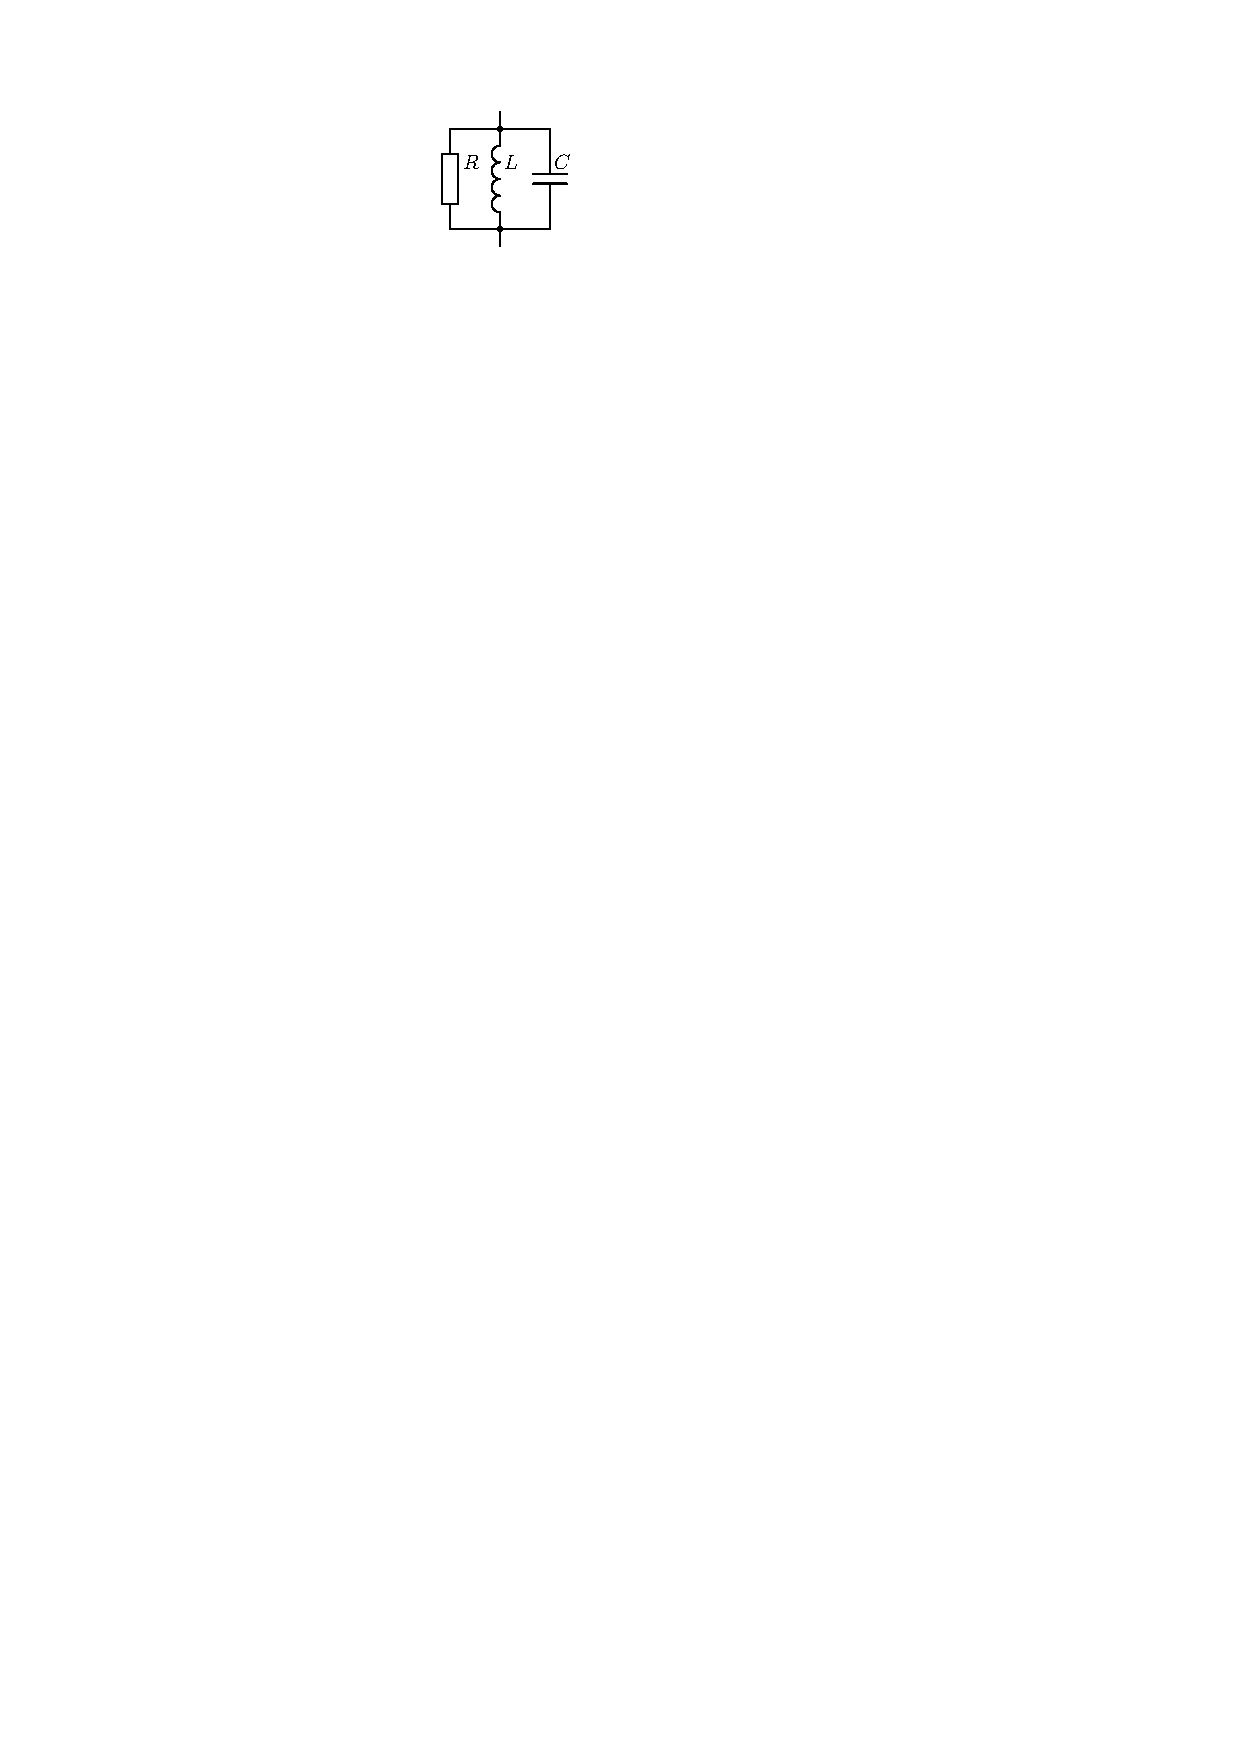
\includegraphics[scale=1.4]{./figs/RLC_circuit.pdf}
  \caption{Ein Parallelschwingkreis bestehend aus dem \textsc{ohm}schen Widerstand~$R$, der Induktivität~$L$ und der Kapazität~$C$ als Modell für die elektrischen Eigenschaften eines Hohlraumresonators in der Nähe einer Resonanz.}
  \label{fig:rlc_circuit}
\end{figure}
Die elektrischen Eigenschaften von Hohlraumresonatoren können in einem beschränkten Frequenzbereich um eine Resonanz durch das Modell des Parallelschwingkreises (siehe Abb.\ \ref{fig:rlc_circuit}) erklärt werden.
Zu dessen vollständiger Beschreibung ist die Angabe der drei Kenngrößen Widerstand~$R$, Induktivität~$L$ und Kapazität~$C$ ausreichend.
Für die Behandlung von Hohlraumresonatoren ist es zweckmäßig, andere Parameter zur Beschreibung zu wählen.
Daher verwendet man stattdessen die Eigenfrequenz~$\omega_0$, die Kreisgüte~$Q_0$ und der Widerstand~$R$ zur Charakterisierung des Schwingkreises.
Die Eigenfrequenz des Kreises folgt aus der \textsc{Thomson}schen Schwingungsgleichung
\begin{align}
  \omega_0 = \frac{1}{\sqrt{L C}}
\end{align}
und die Kreisgüte aus ihrer Definition
\begin{align}
  Q_0 &\coloneqq 2\pi \cdot \frac{\text{gespeicherte Energie}}{\text{Energieverlust pro Periode}} = \frac{\omega_0 W_0}{P_\mathrm{V}} = \omega_0 R C
  \label{eq:def_guete}
\end{align}
mit der im Kreis gespeicherten Energie $W_0$ und der Verlustleistung $P_\mathrm{V}$ aufgrund des \textsc{ohm}schen Widerstandes $R$.
Nach der Einführung dieser Kenngrößen kann die Impedanz $Z(\omega)$ des Kreises beziehungsweise des Hohlraumresonators ausgedrückt werden als
\begin{align}
  Z(\omega) = \left( \frac{1}{R} + \frac{1}{\I \omega L} + \I \omega C \right)^{-1} = \frac{R}{1 + \I Q_0 \left( \frac{\omega}{\omega_0}  - \frac{\omega_0}{\omega}\right)} \eqdot
\end{align}

Bisher war die Betrachtung auf ungetriebene Resonatoren beschränkt und soll nun auf die Anregung durch ein externes Hochfrequenzsignal erweitert werden.
Zur Übertragung dessen Leistung über einen angeschlossenen Wellenleiter mit charakteristischer Impedanz~$Z_0$ an eine Schwingungsmode der Kavität, können verschiedene Methoden verwendet werden.
Eine ist die induktive Kopplung an das Magnetfeld der Mode, bei der der Wellenleiter mit einer Leiterschleife (die sog.\ Koppelschleife) im Resonator verbunden ist.
Dadurch wird in der Leiterschleife ein hochfrequenter Wechselstrom angeregt, welcher ein zeitlich veränderliches Magnetfeld erzeugt. Dieses kann an das Magnetfeld verschiedener Moden der Kavität koppeln und diese anregen.
\begin{figure}[htb]
  \centering
  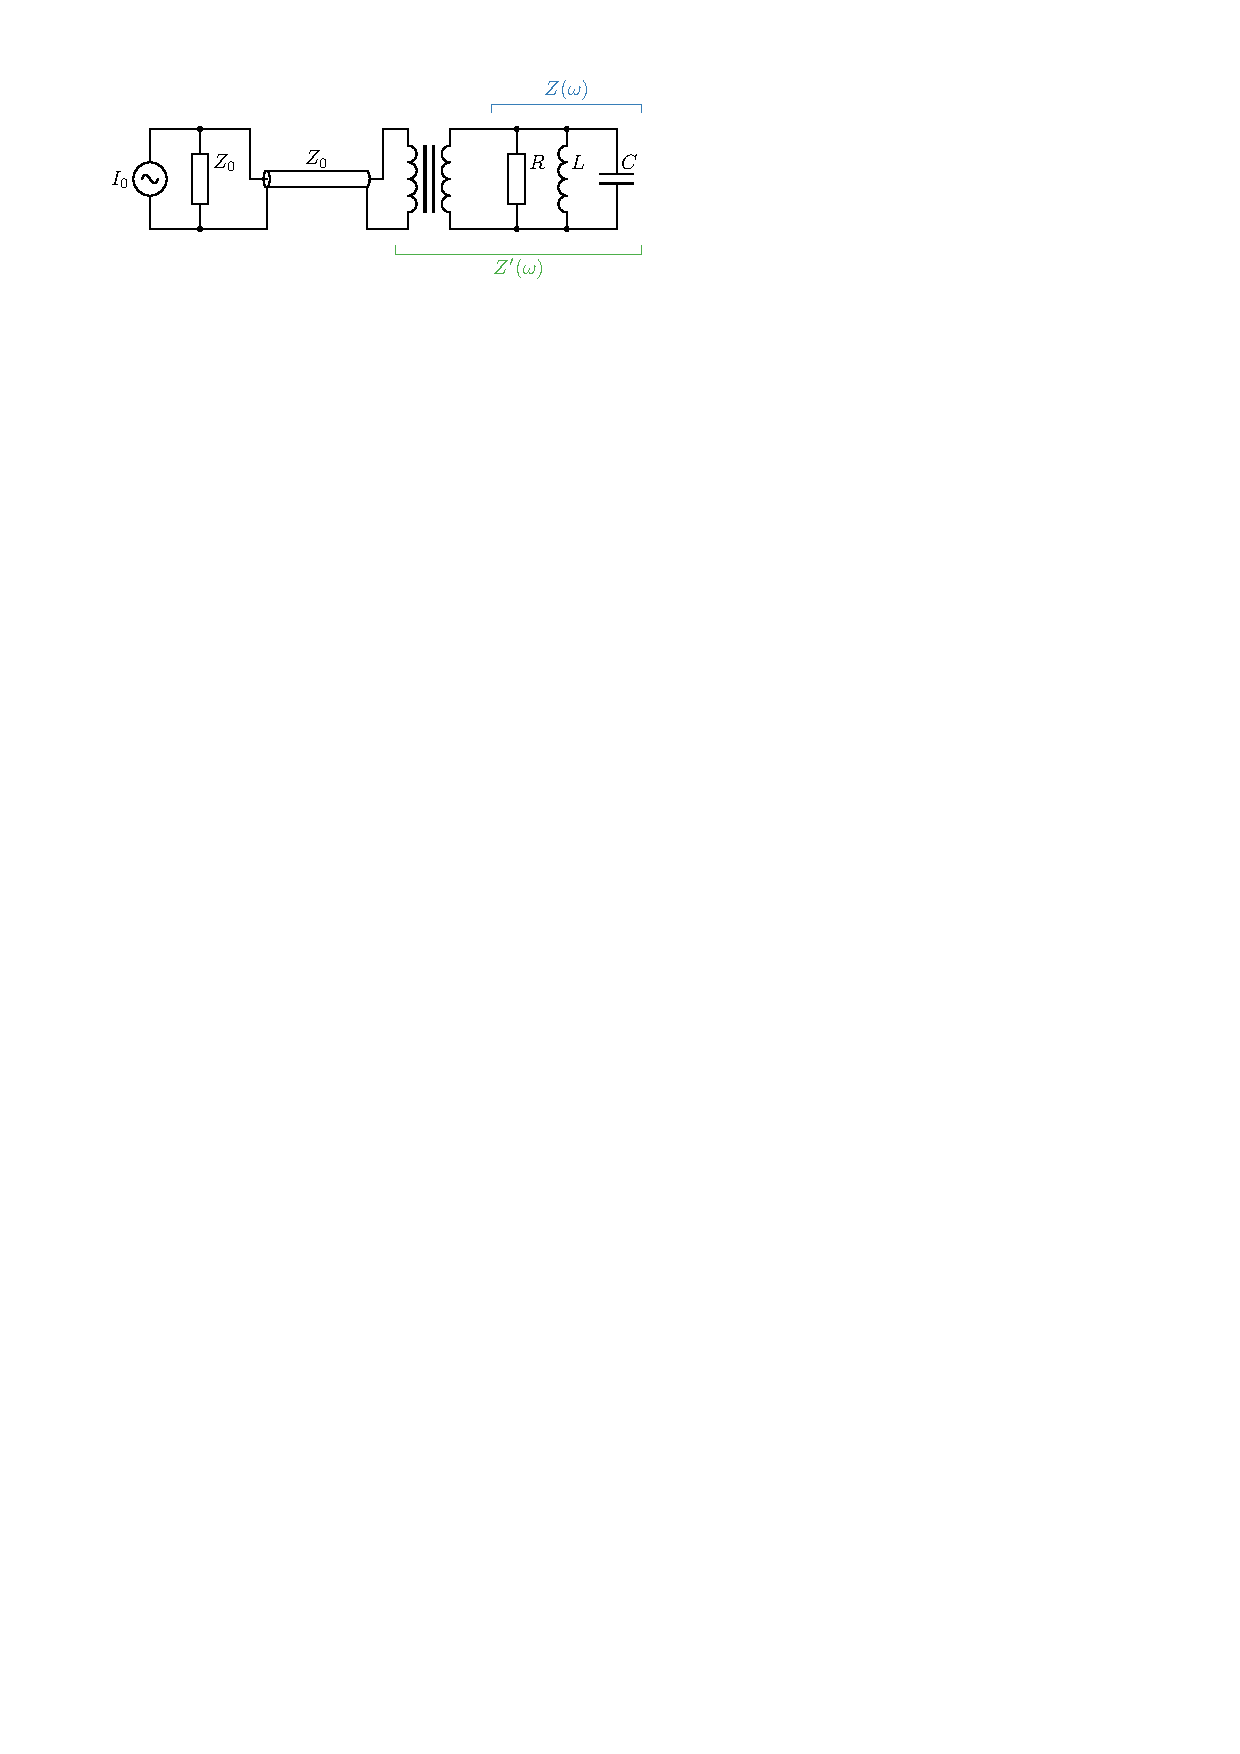
\includegraphics[scale=1.4]{./figs/RLC_coupling.pdf}
  \caption{Modell der induktiven Kopplung eines treibenden Hochfrequenzsignals~$U_0$ über die Koppelschleife an den Resonator. Die Signalquelle ist mit einem Wellenleiter charakteristischer Impedanz~$Z_0$ mit der Koppelschleife verbunden. Die Impedanz des Resonators~$Z$ im Sekundärkreis wird durch die induktive Kopplung zur Impedanz~$Z^\prime$ im Primärkreis transformiert.}
  \label{fig:rlc_coupling}
\end{figure}

Im Modell des Parallelschwingkreises (vgl.\ Abb.\ \ref{fig:rlc_coupling}) bedeutet dies, dass die Impedanz~$Z(\omega)$ der Kavität durch die induktive Kopplung transformiert wird.
Direkt hinter der Koppelschleife habe der Resonator die transformierte Impedanz~$Z^\prime(\omega)$.
Man definiert als Maß für die Kopplung den sog.\ Koppelfaktor
\begin{align}
  \kappa \coloneqq \frac{Z^\prime(\omega_0)}{Z_0}
  \label{eq:koppelfaktor}
\end{align}
mit dem Wellenwiderstand~$Z_0$ des Wellenleiters und unterscheidet zwischen unterkritischer $(\kappa < 1)$, kritischer $(\kappa = 1)$ und überkritischer Kopplung $(\kappa > 1)$.
Im Falle von resonanter Anregung bei kritischer Kopplung folgert man aus Gleichung \eqref{eq:koppelfaktor}, dass der Wellenleiter mit seiner charakteristischen Impedanz abgeschlossen ist und somit keine Reflexionen an der Koppelschleife entstehen.
Mit der Definition des Koppelfaktors und der Proportionalität $Z^\prime(\omega) \propto Z(\omega)$ für ideale Transformatoren folgt die Frequenzabhängigkeit der Impedanz~$Z^\prime(\omega)$ des Systems bestehend aus Koppelschleife und Resonator:
\begin{align}
  Z^\prime(\omega) = \kappa \frac{Z_0}{R} Z(\omega) \eqdot
  \label{eq:impedanz_hinter_schleife}
\end{align}

Von besonderem Interesse ist der komplexe Reflexionskoeffizient zwischen Wellenleiter und Koppelschleife.
Er beschreibt das Verhältnis der komplexen Spannungsamplituden von hin- und rücklaufender Welle in einem Wellenleiter.
Aus der Leitungstheorie \cite[S.\ 57]{pozar} folgt für den Reflexionskoeffizienten~$\rho$ am Übergang von einem Wellenleiter mit Wellenwiderstand~$Z_0$ auf eine Abschlussimpedanz~$Z^\prime$:
\begin{align}
  \rho = \frac{Z^\prime - Z_0}{Z^\prime + Z_0} \eqdot
  \label{eq:reflexionskoeff_trans_line}
\end{align}
Es folgt nach Einsetzen von Gl.~\eqref{eq:impedanz_hinter_schleife} in Gl.~\eqref{eq:reflexionskoeff_trans_line} der Ausdruck für den Reflexionskoeffizienten:
\begin{align}
  \rho(\omega) = \frac{\frac{\kappa}{R} \cdot Z(\omega) - 1}{\frac{\kappa}{R} \cdot Z(\omega) + 1} = \frac{(\kappa - 1) + \I  Q_0 \left( \frac{\omega}{\omega_0}  - \frac{\omega_0}{\omega}\right)}{\left( \kappa + 1 \right) + \I  Q_0 \left( \frac{\omega}{\omega_0}  - \frac{\omega_0}{\omega}\right)}
\end{align}
Diese Gleichung ermöglicht den experimentellen Zugang zur Bestimmung von Koppelfaktor~$\kappa$, Güte~$Q_0$ und Resonanzfrequenz~$\omega_0$ von Hohlraumresonatoren.

%------------------------------------------------------------------------------
\section{Resonante Störkörpermessung}
\label{sec:resonante_stoerkoerpermessung}
%------------------------------------------------------------------------------
Die resonante Störkörpermessung dient der Bestimmung der ortsabhängigen elektrischen und magnetischen Feldamplituden in Hohlraumresonatoren.
Sie basiert auf der Störung des elektromagnetischen Feldes im Resonatorinnenraum durch einen dielektrischen oder magnetischen Körper (dem sog.\ Störkörper), welcher durch das Feld polarisiert beziehungsweise magnetisiert wird.
Eine solche lokalisierte Störung verursacht eine Verschiebung der Resonanzfrequenz~$\Delta \omega$ in Abhängigkeit des elektrischen und magnetischen Feldes am Ort des Störkörpers.
Quantitativ kann die Verschiebung beschrieben werden durch (für eine Herleitung siehe Anhang \ref{app:herleitung_frequenzverschiebung}):
\begin{align}
  \frac{\Delta \omega}{\omega_0} = - \frac{\int_V \mathrm{d}V \left[ \ve_0^* \cdot \vec{P} + \vb_0^* \cdot \vec{M} \right]}{4 W_0}
  \label{eq:frequenzverschiebung}
\end{align}
wobei $V$ das Resonatorvolumen, $\vec{P}$ die Polarisation, $\vec{M}$ die Magnetisierung, $W_0$ die im elektromagnetischen Feld gespeicherte Energie und $\ve_0^*, \vb_0^*$ die komplex konjugierten Felder des ungestörten Resonators sind.

Im Rahmen dieser Arbeit wird eine dielektrische Kugel mit relativer elektrischer Permittivität~$\varepsilon_\mathrm{r}$ verwendet.
Darüber hinaus sei die relative magnetische Permeabilität des Störkörpers $\mu_\mathrm{r} = 1$, sodass die Magnetisierung im externen Feld vernachlässigt werden kann.
Weiterhin wird angenommen, dass das Volumen des kugelförmigen Störkörpers wesentlich kleiner ist als das Resonatorvolumen, sodass am Ort des Störkörpers das elektrische Feld als homogen angesehen werden kann.
Dadurch kann die Polarisation $\vec{P}$ der dielektrischen Kugel im homogenen elektrischen Feld $\ve_0$ ausgedrückt werden als \cite[S.\ 115]{jackson}:
\begin{align}
  \vec{P} = 3 \, \frac{\varepsilon_\mathrm{r} - 1}{\varepsilon_\mathrm{r} + 2} \, \varepsilon_0 \ve_0
  \label{eq:polarisation_kugel}
\end{align}
mit der elektrischen Feldkonstante~$\varepsilon_0$.
Durch die Annahme der Homogenität der Felder am Ort des Störkörpers und verschwindender Polarisation und Magnetisierung außerhalb des Störkörpervolumens~$V_\mathrm{s}$, kann von der Integration über das Resonatorvolumen~$V$ in Gleichung \eqref{eq:frequenzverschiebung} zur Integration über das Störkörpervolumen übergangen werden.
Nach Einsetzen der Polarisation der dielektrischen Kugel in Gleichung \eqref{eq:frequenzverschiebung} folgt für die Amplitude des elektrischen Feldes am Ort des Störkörpers $(x_\mathrm{s}, y_\mathrm{s}, z_\mathrm{s})$:
\begin{align}
  |\ve_0(x_\mathrm{s}, y_\mathrm{s}, z_\mathrm{s})| = \sqrt{-4 \cdot \frac{W_0}{\alpha_\mathrm{s}} \cdot \frac{\Delta \omega}{\omega_0}} \qquad \text{für} \qquad \Delta \omega \leq 0
  \label{eq:skm_e_feld}
\end{align}
(folglich durch $|\ve_0|$ abgekürzt) und der Störkörperkonstanten~$\alpha_\mathrm{s}$ für sphärische Störkörper:
\begin{align}
  \alpha_\mathrm{s} \coloneqq 3 \, \frac{\epsilon_\mathrm{r} - 1}{\epsilon_\mathrm{r} + 2} \, \epsilon_0 V_\mathrm{s} \eqdot
\end{align}
Um die Amplitude des elektrischen Feldes unabhängig von der im Resonator gespeicherten Energie~$W_0$ angeben zu können, verwendet man die Definition der Güte~$Q_0$ in Gleichung \eqref{eq:def_guete} und normiert das elektrische Feld auf die Wurzel der Verlustleistung~$P_\mathrm{V}$ des Resonators:
\begin{align}
  \frac{|\ve_0|}{\sqrt{P_\mathrm{V}}} = \sqrt{-4 \cdot \frac{Q_0}{\alpha_s} \cdot \frac{\Delta \omega}{\omega_0^2}}
  \label{eq:skm_e_feld_normiert}
\end{align}
Diese Größe ist unabhängig von der in den Resonator eingekoppelten Leistung und dient als Basis für die folgenden Berechnungen.


%------------------------------------------------------------------------------
\section{Charakteristische Größen von Beschleunigungsresonatoren}
\label{sec:resonator_charakteristiken}
%------------------------------------------------------------------------------
Eine wichtige Kenngrößen von Moden in Beschleunigungsresonatoren ist die Beschleunigungsspannung~$U$, die ein Teilchen erfährt, das einen Resonator der Länge~$L$ instantan durchquert:
\begin{align}
  U = \int_0^L |\ve_0 (z)| \, \mathrm{d}z \eqdot
\end{align}
Um den effektiven Energiegewinn eines Teilchens zu erhalten, muss die endliche Geschwindigkeit des Teilchens und die harmonische Zeitabhängigkeit des Feldes beachtet werden.
Dazu definiert man den Laufzeitfaktor~$\Lambda$ für ultrarelativistische Teilchen ($v = c$):
\begin{align}
  \Lambda = \left| \frac{ \int_0^L |\ve_0(z)| \cdot \sin\left( \frac{\omega_0}{c} z + \varphi_0 \right) \, \mathrm{d}z }{ \int_0^L |\ve_0(z)| \, \mathrm{d}z } \right| \eqcomma
  \label{eq:laufzeitfaktor}
\end{align}
wobei die Phase $\varphi_0$ so zu wählen ist, dass der Laufzeitfaktor maximiert wird.
Dadurch erhält man die effektive Beschleunigungsspannung~$U_\mathrm{eff}$:
\begin{align}
  U_\mathrm{eff} = \Lambda \cdot U
\end{align}
und damit die Änderung der Energie eines ultrarelativistischen Teilchens der Ladung $q$ beim Passieren des Resonators $\Delta E = q \cdot U_\mathrm{eff}$.
Darüber hinaus definiert man als Maß für die Effizienz der Beschleunigung die sog.\ Shuntimpedanz~$R_\mathrm{S}$:
\begin{align}
  R_\mathrm{S} = \frac{U^2}{2 P_\mathrm{V}}
\end{align}
mit der in den Resonatorwänden dissipierten Leistung $P_\mathrm{V}$ und analog die effektive Shuntimpedanz~$R_\mathrm{S}^\mathrm{eff}$:
\begin{align}
  R_\mathrm{S}^\mathrm{eff} = \frac{U_\mathrm{eff}^2}{2 P_\mathrm{V}} = \Lambda^2 \cdot R_\mathrm{S} \eqdot
\end{align}
In Abhängigkeit der im Resonator angeregten Moden unterscheidet man zwischen longitudinaler und transversaler Beschleunigungsspannung/Shuntimpedanz.
Dies liegt darin begründet, dass TM-Moden nur elektrische Felder mit longitudinaler und TE-Moden mit transversaler Ausrichtung aufweisen und dementsprechend nur zur longitudinalen/transversalen Beschleunigung der Teilchen führen.

\todo{Verlustfaktor?, R/Q, R/(Q*L)}
%$R$ über $Q_0$\footnote{Unabhängig von Verlusten, nur Geometrieabhängig}: $R_\mathrm{S}/Q_0$

%==============================================================================
\chapter{Aufbau und Methodik}
\label{sec:aufbau_und_methodik}
%==============================================================================


%------------------------------------------------------------------------------
\section{Der PETRA-Resonator}
%------------------------------------------------------------------------------
\begin{figure}[htb]
  \centering
  \includegraphics[width=0.8\textwidth]{./figs/cavity/cavity.pdf}
  \caption{Schematischer Darstellung des Querschnitts eines siebenzelligen PETRA-Resonators mit Koppelschleife und zwei Abstimmstempeln. Der Abstand zwei benachbarter Zellenmitten beträgt \SI{30}{\centi\metre} und die Gesamtlänge \SI{222}{\centi\metre}.}
  \label{fig:petra_cavity}
\end{figure}
Im Rahmen dieser Arbeit wird das elektrische Feld von zwei siebenzelligen Beschleunigungsresonatoren vom Typ PETRA \cite{desy_petra} vermessen, welche in Kooperation von DESY und Balzers Hochvakuum GmbH (1982/83) hergestellt wurden.
Der Resonator ist ausgelegt auf die Beschleunigung von ultrarelativistischen Elektronen und Positronen durch die $\mathrm{TM}_{010}$-Mode bei einer Frequenz von \SI{499.67}{MHz}.
Der Querschnitt dieser Kavität ist in Abbildung \ref{fig:petra_cavity} schematisch dargestellt.
Die einzelnen Zellen werden durch leitende Kupferwände voneinander getrennt, wobei deren spezielle Form der Maximierung des Laufzeitsfaktors \eqref{eq:laufzeitfaktor} dient.
Jede der Zellen des PETRA-Resonators stellt einen Hohlraumresonator dar, der durch vier Koppelschlitze in der trennenden Kupferwand an die jeweiligen Nachbarzellen gekoppelt ist.
Dies führt zur Aufspaltung jeder Mode der Einzelzelle in $N$ Moden der Resonatorkette\footnote{Dies ist analog zu gekoppelten mechanischen Pendeln, welche ebenfalls verschiedene Schwingungsmoden aufweisen.}, wobei $N = 7$ die Anzahl der Zellen ist.
Die $N$ Moden der Resonatorkette unterscheiden sich neben der Resonanzfrequenz $\omega_0$ auch im Phasenvorschub $\Delta \varphi$ zwei benachbarter Zellen.
Die Benennung der Moden der Resonatorkette erfolgt nach ihrem Phasenvorschub $\Delta \varphi$ (z.B.\ $\pi$-Mode für $\Delta \varphi = \pi$) und die für den siebenzelligen PETRA-Resonator möglichen Moden sind:
\begin{align}
  \Delta \varphi = 0,\; \frac{1}{6} \pi,\; \frac{1}{3} \pi,\; \frac{1}{2} \pi,\; \frac{2}{3} \pi,\; \frac{5}{6} \pi,\; \pi
\end{align}
In der mittleren Zelle des PETRA-Resonators befindet sich die Koppelschleife \cite{desy_schleife}, deren Geometrie auf den Resonator angepasst ist um eine kritische Kopplung an die $\mathrm{TM}_{010}$-Beschleuniger\-mode zu ermöglichen.
Eine Anpassung des Koppelfaktors kann durch Drehen der Schleife erreicht werden, da dies die effektive Fläche der Leiterschleife senkrecht zum Magnetfeld der betrachteten Resonatormode verändert.
In den Zellen~2 und 6 sind Abstimmstempel \cite{desy_stempel} angebracht die durch Schrittmotoren in bzw.\ aus der Kavität gefahren werden können.
Das Verstellen der Stempel führt zu einer Änderung der Geometrie des Resonators und folglich zu einer Verschiebung der Resonanzfrequenz.
Dies kann zum Stimmen der Resonanzfrequenz einer Mode in einem beschränkten Frequenzbereich genutzt werden.
Die zwei weiteren Vakuumflansche in den Zellen~1 und 7 dienen dem Anschluss von Vakuumpumpen.


Die in dieser Arbeit vermessenen Resonatoren seien im Folgenden mit PETRA-III und -IV bezeichnet\footnote{Die fünfzelligen Resonatoren PETRA-I und -II sind im Stretcherring von ELSA verbaut.}. Der Resonator PETRA-IV wurde durch eine Gasentladung gereinigt.


%------------------------------------------------------------------------------
\section{Aufbau des Störkörpermessstandes}
%------------------------------------------------------------------------------
\begin{sidewaysfigure}[p]
	\centering
	\includegraphics[width=1.0\textheight]{./figs/cavity/messaufbau.pdf}
	\caption{Schematischer Aufbau des Störkörpermessstandes für einen siebenzelligen PETRA-Resonator mit Abstimmstemplen und Einkoppelschleife (a), Montageträger (b), Gestell aus einem Aluminiumprofilsystem (c), Kreuzblenden (d), Polytetrafluorethylen-Störkörper (e), Spindel mit Schrittmotor (f) und Zugfeder (g).}
	\label{fig:stoerkoerpermessstand}
\end{sidewaysfigure}
Zur Bestimmung des elektrischen Feldes auf der Strachachse des Resonators wird die in Abschnitt \ref{sec:resonante_stoerkoerpermessung} eingeführte resonante Störkörpermessung ausgenutzt.
Dazu wird ein kugelförmiger Störkörper mit dem Durchmesser $D = \SI{20.05 +- 0.02}{mm}$ durch eine zentrische Bohrung des Durchmessers $d = \SI{1.3 +- 0.05}{mm}$ auf einem reißfesten Kunststofffaden befestigt.
Wegen der verschwindenden magnetischen Suszeptibilität wurde der Störkörper aus Polytetrafluorethylen (Teflon\textsuperscript{\textregistered}) gefertigt, was die Verwendung von Gleichung \eqref{eq:skm_e_feld_normiert} für dielektrische Kugeln zur Bestimmung des Amplitude des elektrischen Feldes im Resonator erlaubt.
Um diesen Störkörper auf der Strahlachse durch den Resonator bewegen zu können, wurde der Störkörpermessstand aus Abbildung \ref{fig:stoerkoerpermessstand} aufgebaut.
Dieser besteht aus dem siebenzelligen PETRA-Resonator, welcher fest auf einem Montageträger befestigt wurde.
Ein Gestell aus einem Aluminiumprofilsystem, welches fest mit dem Träger verbunden wurde, dient der Befestigung der weiteren Komponenten des Messstandes.
Über ein System von Umlenkrollen kann der Kunststofffaden durch die Kavität geführt werden und schließlich beidseitig fest mit einer Aluminiumspindel verbunden werden, die wiederum auf der Welle eines Schrittmotors befestigt ist.
Die Rückführung des Fadens auf die Spindel führt dazu, dass unabhängig von der Spannung des Fadens das Drehmoment auf der Welle des Schrittmotors kompensiert wird.
Darüber hinaus verhindert die feste Verbindung des Fadens mit der Spindel ein longitudinales Verrutschen des Fadens in seiner Führung, was insbesondere für eine präzise Ortsbestimmung des Störkörpers relevant ist.

Durch das Auf- beziehungsweise Abrollen des Fadens auf der Spindel, kann der Störkörper entlang der Strahlachse verschoben werden.
Die Drehung der Spindel erfolgt dabei durch den 2-Phasen Schrittmotor \textit{MDrive\textsuperscript{\textregistered} 23 Plus Motion Control} des Herstellers \textit{Schneider Electric} \cite{motor_datasheet}.
Der Motor besitzt eine integrierte Steuereinheit, welche die direkte Ansteuerung über eine serielle Schnittstelle ermöglicht.
Ein voller Schritt des Motors entspricht einem Drehwinkel der Welle von \SI{1.8}{\degree} oder \num{200} Schritten pro Umdrehung.
Durch eine spezielle Ansteuerungstechnik, welche in der Steuereinheit implementiert wurde, wird ein Schritt zusätzlich in \num{256} sogenannte \textit{Microsteps} eingeteilt.
Die Ortsinformation des Störkörpers entlang der Strahlachse kann dann aus der Anzahl der erfolgten Microsteps gewonnen werden.
Aus der Geometrie der Spindel folgt für die zugehörige Proportionalitätskonstante \SI{0.005996}{\milli\metre\per\micro\step}.
Die Stellgenauigkeit \todo{nicht additiv} des Schrittmotors liegt jedoch weit über der durch \textit{Microstepping} erreichbaren Auflösung und liegt typischerweise bei \SI{5}{\percent} eines vollen Schrittes.
Dies entspricht einem Winkelfehler von \SI{0.09}{\degree} oder einem Fehler in der Störkörperposition von weniger als \SI{0.1}{\milli\metre}.
\todo{Dadurch ist eine Positionierung des Störkörpers im Millimeterbereich möglich.}

Zur Bestimmung der Resonanzfrequenz und Güte des Resonators dient der vektorielle Netzwerkanalysator \textit{Rohde \& Schwarz: ZVC 1127.8600.62}, welcher über ein \SI{50}{\ohm}-Koaxialkabel (RG~214/U) mit der Koppelschleife verbunden wird.
Die Verbindung erfolgt dabei über einen Spezialadapter vom Typ-N Stecker des Kabels auf die $6\tfrac{1}{8}$-Zoll \SI{50}{\ohm}-Koaxialverbindung der Koppelschleife.
Der VNA erzeugt ein sinusförmiges Signal variabler Frequenz und einer Leistung von \SI{6}{dBm}, welches an der Koppelschleife teilweise reflektiert wird.
Ein Richtkoppler im VNA trennt das reflektierte vom ausgehenden Signal und ermöglicht eine Bestimmung des komplexen Reflexionsfaktors durch einen Vergleich von Phase und Leistung beider Signale.
Um ein von der Dämpfung und Laufzeit im Koaxialkabel unabhängiges Ergebnis zu erhalten, kann eine Kalibration durchgeführt werden, indem das Ende der Messleitung durch einen offenen, kurzgeschlossenen und \SI{50}{\ohm}-Abschluss terminiert wird.
Der verwendete VNA ermöglicht die Messung des Reflexionsfaktors an bis zu \num{2001} gleichverteilten Messpunkten auf einem vorgegebenen Frequenzintervall.
Die Eingabe und Ausgabe erfolgt auch hier durch eine serielle Schnittstelle.
\todo{AVG, Marker etc.?}

Zur Realisierung einer automatisierten Störkörpermessung und der Koordination von Schrittmotor und Netzwerkanalysator dient der Mikrocomputer \textit{Raspberry Pi} (RPi), der mit den Komponenten des Messaufbaus über serielle Schnittstellen kommunizieren kann.
In der Programmiersprache \textit{Python} wurde dazu die serielle Kommunikation mit Motor und VNA, sowie die Steuerung des Messablaufs implementiert.
Der genaue Ablauf einer Störkörpermessung wird im nächsten Abschnitt erläutert.

\todo{Einfluss des Fadens?, Durchhängen des Fadens}


%------------------------------------------------------------------------------
\section{Messmethodik}
%------------------------------------------------------------------------------

\subsection{Temperatur}
Volumenänderung $\nu$, Leitfähigkeitänderung $Q$

Fit der Resonanzkurve an die Güte\\
Resonanzfrequenz aus dem Minimum der Resonanzkurve\\
Längenmessung\\
Checkmode\\
Einschwingzeit

%------------------------------------------------------------------------------
\chapter{Störkörpermessungen}
\label{sec:stoerkoerpermessung}
%------------------------------------------------------------------------------


%------------------------------------------------------------------------------
\section{Vorbereitung der Störkörpermessung}
%------------------------------------------------------------------------------

%------------------------------------------------------------------------------
\subsection{Vorbereitung des Resonators}
\label{sec:vorbereitung_resonator}
%------------------------------------------------------------------------------
Bevor mit der Störkörpermessung nach Abschnitt \ref{sec:messmethodik} begonnen werden kann, müssen noch Einstellungen am Resonator erfolgen.
Zum einen wird die Koppelschleife so gedreht, dass eine nahezu kritische Einkopplung ($\kappa \approx 1$) an die $\mathrm{TM}_{010}\text{-}\pi$-Mode des Resonators realisiert wird.
Dies kann durch eine Messung des Reflexionskoeffizienten mit dem VNA überprüft werden, da für den Fall kritischer Kopplung gemäß Gleichung \eqref{eq:resonanzkurve}
\begin{align}
	|\rho(\omega = \omega_0)| = 0
\end{align}
gilt.

Außerdem werden beide Abstimmstempel so eingestellt, dass sich eine symmetrische Feldverteilung im Resonator ausbildet.
Dazu wird die Resonanzfrequenzverschiebung durch den Störkörper in der Mitte beider Stempel-Zellen gemessen.
Ist die Frequenzverschiebung und somit auch die Amplitude elektrischen Feldes an beiden Stellen gleich, so liegt eine symmetrische Feldverteilung vor.
Anderenfalls werden die Stempel solange gegeneinander Verfahren, bis eine Stempelstellung gefunden wurde, für die sich ein symmetrisches Feld im Resonator ausbildet.

Schließlich muss die Beschleunigungsmode auf ihre Sollfrequenz im Vakuum von $\SI{499.67}{MHz}$ durch paralleles Verfahren der Stempel abgestimmt werden.
Dabei ist zu beachten, dass die Luft im Hohlraum des Resonators zu einer zusätzlichen Verstimmung führt.
Ist der Resonator durch ein Medium der relativen Permittivität~$\varepsilon_\mathrm{r}$ und Permeabilität~$\mu_\mathrm{r}$ ausgefüllt, so kann die Verstimmung der Resonanzfrequenzen durch
\begin{align}
	\nu_0^\mathrm{Med.} = \frac{\nu_0^\mathrm{Vak.}}{\sqrt{\varepsilon_\mathrm{r} \mu_\mathrm{r}}}
	\label{eq:resonanzfrequenz_medium}
\end{align}
beschrieben werden \cite{pusch}.
Mit der relativen Permittivität trockener Luft~$\varepsilon_\mathrm{r}^\mathrm{Luft} = \num{1.0005364}$ unter Normalbedingungen \cite[S.\ 1093]{CRC}, vernachlässigbarer relativer Permeabilität~($\mu_\mathrm{r} \approx 1$) und der Sollfrequenz im Vakuum~$\nu_0^\mathrm{Vak.}$ folgt die Frequenz der Beschleunigungsmode
\begin{align}
	\nu_0^\mathrm{Luft} = \SI{499.54}{MHz}
\end{align}
für den luftgefüllten Resonator.
Da diese Frequenz mit Temperatur und Luftfeuchtigkeit variiert, ist ein exaktes Abstimmen auf diese Frequenz nicht zweckmäßig und es genügt die grobe Einstellung mit einer Genauigkeit von einigen \si{\kilo\hertz}.

%------------------------------------------------------------------------------
\subsection{Bestimmung der Störkörperkonstante}
%------------------------------------------------------------------------------

Zur Berechnung der Störkörperkonstante~$\alpha_\mathrm{s}$ des kugelförmigen Störkörpers aus PTFE mit einem Durchmesser $D = \SI{20.05 +- 0.05}{mm}$ und der zentrischen Bohrung mit Durchmesser $d = \SI{1.3 +- 0.05}{mm}$ kann Gleichung \eqref{eq:stoerkoerperkonstante} verwendet werden.
Die relative Permittivität von PTFE beträgt im Mittel $\varepsilon_\mathrm{r} = \num{2.1}$ und variiert mit der Dichte und Kristallinität des Materials \cite[S.\ 2201]{CRC}.
Daher wird für den verwendeten Störkörper $\varepsilon_\mathrm{r} = \num{2.1 +- 0.05}$ angenommen.
Es folgt für die Störkörperkonstante
\begin{align}
	\alpha_\mathrm{s} = \SI{2.99 +- 0.11e-17}{\ampere\second\metre\squared\per\volt} \eqcomma
	\label{eq:stoerkoerperkonstante_ptfe}
\end{align}
wobei das fehlende Volumen der zentrischen Bohrung beachtet wurde.

Bei der Bestimmung der elektrischen Felder gemäß Gleichung \eqref{eq:skm_e_feld_normiert}, wirkt der Fehler der Störkörperkonstanten systematisch auf das resultierende Feld.
Dieser systematische Einfluss muss insbesondere bei der Integration des Feldes über die Störkörperposition (Bestimmung von Beschleunigungsspannung und Shuntimpedanz) gesondert betrachtet werden.
Um diesen Fehler zu verringern, könnte eine direkte Bestimmung der Störkörperkonstanten in einem Referenzresonator durchgeführt werden.
Darauf wurde jedoch in dieser Arbeit verzichtet, da mit einem relativen Fehler von unter $\SI{4}{\percent}$ eine ausreichende Genauigkeit vorliegt.

%------------------------------------------------------------------------------
\subsection{Bestimmung von Resonanzfrequenz und Güte}
\label{sec:resfreq_guete}
%------------------------------------------------------------------------------
Die Bestimmung von Resonanzfrequenz und Güte der Resonatormoden kann anhand des gemessenen Reflexionsspektrums der jeweiligen Resonanz erfolgen.
Dazu wird eine Kurve gemäß Gleichung \eqref{eq:resonanzkurve} nach der Methode der kleinsten Quadrate an das gemessene Spektrum angepasst.
Dies wird, am Beispiel der $\mathrm{TM}_{010}\text{-}\pi$-Beschleunigungsmode von PETRA-III, in Abbildung \ref{fig:guetefit} dargestellt.
\begin{figure}[htb]
  \centering
  % GNUPLOT: LaTeX picture with Postscript
\begingroup
  \makeatletter
  \providecommand\color[2][]{%
    \GenericError{(gnuplot) \space\space\space\@spaces}{%
      Package color not loaded in conjunction with
      terminal option `colourtext'%
    }{See the gnuplot documentation for explanation.%
    }{Either use 'blacktext' in gnuplot or load the package
      color.sty in LaTeX.}%
    \renewcommand\color[2][]{}%
  }%
  \providecommand\includegraphics[2][]{%
    \GenericError{(gnuplot) \space\space\space\@spaces}{%
      Package graphicx or graphics not loaded%
    }{See the gnuplot documentation for explanation.%
    }{The gnuplot epslatex terminal needs graphicx.sty or graphics.sty.}%
    \renewcommand\includegraphics[2][]{}%
  }%
  \providecommand\rotatebox[2]{#2}%
  \@ifundefined{ifGPcolor}{%
    \newif\ifGPcolor
    \GPcolortrue
  }{}%
  \@ifundefined{ifGPblacktext}{%
    \newif\ifGPblacktext
    \GPblacktexttrue
  }{}%
  % define a \g@addto@macro without @ in the name:
  \let\gplgaddtomacro\g@addto@macro
  % define empty templates for all commands taking text:
  \gdef\gplbacktext{}%
  \gdef\gplfronttext{}%
  \makeatother
  \ifGPblacktext
    % no textcolor at all
    \def\colorrgb#1{}%
    \def\colorgray#1{}%
  \else
    % gray or color?
    \ifGPcolor
      \def\colorrgb#1{\color[rgb]{#1}}%
      \def\colorgray#1{\color[gray]{#1}}%
      \expandafter\def\csname LTw\endcsname{\color{white}}%
      \expandafter\def\csname LTb\endcsname{\color{black}}%
      \expandafter\def\csname LTa\endcsname{\color{black}}%
      \expandafter\def\csname LT0\endcsname{\color[rgb]{1,0,0}}%
      \expandafter\def\csname LT1\endcsname{\color[rgb]{0,1,0}}%
      \expandafter\def\csname LT2\endcsname{\color[rgb]{0,0,1}}%
      \expandafter\def\csname LT3\endcsname{\color[rgb]{1,0,1}}%
      \expandafter\def\csname LT4\endcsname{\color[rgb]{0,1,1}}%
      \expandafter\def\csname LT5\endcsname{\color[rgb]{1,1,0}}%
      \expandafter\def\csname LT6\endcsname{\color[rgb]{0,0,0}}%
      \expandafter\def\csname LT7\endcsname{\color[rgb]{1,0.3,0}}%
      \expandafter\def\csname LT8\endcsname{\color[rgb]{0.5,0.5,0.5}}%
    \else
      % gray
      \def\colorrgb#1{\color{black}}%
      \def\colorgray#1{\color[gray]{#1}}%
      \expandafter\def\csname LTw\endcsname{\color{white}}%
      \expandafter\def\csname LTb\endcsname{\color{black}}%
      \expandafter\def\csname LTa\endcsname{\color{black}}%
      \expandafter\def\csname LT0\endcsname{\color{black}}%
      \expandafter\def\csname LT1\endcsname{\color{black}}%
      \expandafter\def\csname LT2\endcsname{\color{black}}%
      \expandafter\def\csname LT3\endcsname{\color{black}}%
      \expandafter\def\csname LT4\endcsname{\color{black}}%
      \expandafter\def\csname LT5\endcsname{\color{black}}%
      \expandafter\def\csname LT6\endcsname{\color{black}}%
      \expandafter\def\csname LT7\endcsname{\color{black}}%
      \expandafter\def\csname LT8\endcsname{\color{black}}%
    \fi
  \fi
    \setlength{\unitlength}{0.0500bp}%
    \ifx\gptboxheight\undefined%
      \newlength{\gptboxheight}%
      \newlength{\gptboxwidth}%
      \newsavebox{\gptboxtext}%
    \fi%
    \setlength{\fboxrule}{0.5pt}%
    \setlength{\fboxsep}{1pt}%
\begin{picture}(6802.00,4534.00)%
    \gplgaddtomacro\gplbacktext{%
      \csname LTb\endcsname%
      \put(814,704){\makebox(0,0)[r]{\strut{}0{,}0}}%
      \csname LTb\endcsname%
      \put(814,1417){\makebox(0,0)[r]{\strut{}0{,}2}}%
      \csname LTb\endcsname%
      \put(814,2130){\makebox(0,0)[r]{\strut{}0{,}4}}%
      \csname LTb\endcsname%
      \put(814,2843){\makebox(0,0)[r]{\strut{}0{,}6}}%
      \csname LTb\endcsname%
      \put(814,3556){\makebox(0,0)[r]{\strut{}0{,}8}}%
      \csname LTb\endcsname%
      \put(814,4269){\makebox(0,0)[r]{\strut{}1{,}0}}%
      \csname LTb\endcsname%
      \put(1835,484){\makebox(0,0){\strut{}499{,}48}}%
      \csname LTb\endcsname%
      \put(3200,484){\makebox(0,0){\strut{}499{,}50}}%
      \csname LTb\endcsname%
      \put(4565,484){\makebox(0,0){\strut{}499{,}52}}%
      \csname LTb\endcsname%
      \put(5930,484){\makebox(0,0){\strut{}499{,}54}}%
    }%
    \gplgaddtomacro\gplfronttext{%
      \csname LTb\endcsname%
      \put(176,2486){\rotatebox{-270}{\makebox(0,0){\strut{}Reflektionskoeffizient $|\rho|$}}}%
      \put(3675,154){\makebox(0,0){\strut{}Frequenz $\nu$ / \si{MHz}}}%
      \csname LTb\endcsname%
      \put(5418,1097){\makebox(0,0)[r]{\strut{}Messpunkte}}%
      \csname LTb\endcsname%
      \put(5418,877){\makebox(0,0)[r]{\strut{}Anpassung}}%
    }%
    \gplbacktext
    \put(0,0){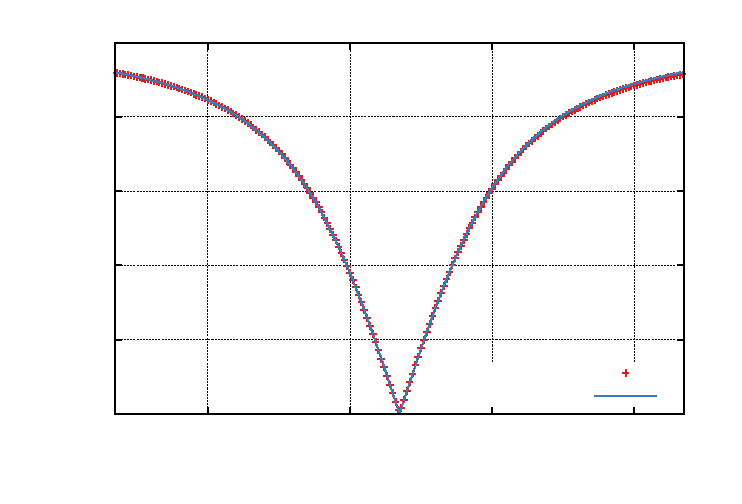
\includegraphics{./plots/guete_fit_pi}}%
    \gplfronttext
  \end{picture}%
\endgroup

  \caption[Anpassung der Resonanzkurve an das Reflexionsspektrum der $\mathrm{TM}_{010}~\pi$-Mode von PETRA-III]{Anpassung der Resonanzkurve~\eqref{eq:resonanzkurve} an ein gemessenes Reflexionsspektrum der $\mathrm{TM}_{010}\text{-}\pi$-Mode von PETRA-III. Aus Gründen der Übersicht wurde nur jeder 10.\ Messpunkt des VNA aufgetragen. Die Anpassung liefert die Resonanzfrequenz~$\nu_0 = \SI{499.537}{MHz}$ (Anpassungsfehler vernachlässigbar), Güte~$Q_0 = \num{29560 +- 20}$ und den Koppelfaktor~$\kappa = \num{1.013 +- 0.001}$.}
  \label{fig:guetefit}
\end{figure}
Um eine bessere Abschätzung der Fehler zu erlauben, wurden zu jeder Resonatormode mehrere Reflexionsspektren aufgenommen und an jedes Spektrum eine Anpassung durchgeführt.
Die resultierenden Ergebnisse folgen aus der Bildung des Mittelwerts der angepassten Parameter.
Da die Resonanzfrequenz der Moden mit der Temperatur der Kavität schwankt, wird auf eine Angabe des Fehlers verzichtet.
Darüber hinaus kann der Einfluss von dielektrischen Verlusten der Luft auf die Güte des Resonators \cite{pozar} vernachlässigt werden.

%------------------------------------------------------------------------------
\section{Vermessung der $\mathrm{TM}_{010}$-Resonatormoden}
\label{sec:tm010_messung}
%------------------------------------------------------------------------------
Die folgenden Abschnitte widmen sich der Auswertung der Störkörpermessungen an den $\mathrm{TM}_{010}$-Resonatormoden von PETRA-III und PETRA-IV, welche gemäß Abschnitt \ref{sec:messmethodik} durchgeführt wurden.
Für beide Resonatoren wurden die $\pi,\, 2/3~\pi, \, 1/3~\pi$ und $0$-Moden vermessen.
Die restlichen Moden der siebenzelligen Resonatorkette, die nach den Erläuterungen in Abschnitt \ref{sec:petra_resonator} erwartet werden, konnten nicht vermessen werden.
Dies ist der Fall, da diese Moden ein verschwindendes elektrisches und magnetisches Feld in der mittleren Zelle des Resonators aufweisen (vgl.\ Abb.\ \ref{fig:spektrum_tm010} f.) und daher nicht oder nur schwach über die Koppelschleife angeregt werden können.

Beide Resonatoren wurden mit einer Schrittweite des Störkörpers von \SI{5}{mm} vermessen, was \num{60} Messpunkten pro Zelle entspricht.
Dadurch sind die gemessenen Feldverteilungen durch das Ortsauflösungsvermögen des verwendeten Störkörpers begrenzt.

\subsection{Auswertung der Messdaten}
Nachdem die Güte~$Q_0$, Resonanzfrequenz~$\nu_0$ und Störkörperkonstante~$\alpha_\mathrm{s}$ bestimmt wurde, kann die Amplitude des elektrischen Feldes (normiert auf die Wurzel der Verlustleistung $P_\mathrm{V}$) gemäß Gleichung \eqref{eq:skm_e_feld_normiert} berechnet werden.
Außerdem kann das effektive elektrische Feld, das ein ultrarelativistisches Teilchen erfährt, welches den Resonator passiert, berechnet und somit der Laufzeitfaktor~$\Lambda$ aus Gleichung \eqref{eq:laufzeitfaktor} bestimmt werden.
Dazu muss neben der harmonischen Zeitabhängigkeit auch die Phasenbeziehung (vgl.\ Abb.\ \ref{fig:phasenbeziehung}) zwischen den einzelnen Zellen beachtet werden.
Darüber hinaus wird die Eintrittsphase des Teilchens in den Resonator so gewählt, dass der Laufzeitfaktor~$\Lambda$ bzw.\ die effektive Shuntimpedanz~$R_\mathrm{S}^\mathrm{eff}$ maximiert wird.

Dies wurde am Beispiel der $\pi$-Mode des PETRA-III Resonators in Abbildung \ref{fig:bsp_feld_tm010pi_petra3} dargestellt.
Im Anhang \ref{app:tm010_felder} wurden die Felder aller vermessenen $\mathrm{TM}_{010}$-Resonatormoden beider Resonatoren zusammengestellt.  
\begin{figure}[h]
	\centering
	% GNUPLOT: LaTeX picture with Postscript
\begingroup
  \makeatletter
  \providecommand\color[2][]{%
    \GenericError{(gnuplot) \space\space\space\@spaces}{%
      Package color not loaded in conjunction with
      terminal option `colourtext'%
    }{See the gnuplot documentation for explanation.%
    }{Either use 'blacktext' in gnuplot or load the package
      color.sty in LaTeX.}%
    \renewcommand\color[2][]{}%
  }%
  \providecommand\includegraphics[2][]{%
    \GenericError{(gnuplot) \space\space\space\@spaces}{%
      Package graphicx or graphics not loaded%
    }{See the gnuplot documentation for explanation.%
    }{The gnuplot epslatex terminal needs graphicx.sty or graphics.sty.}%
    \renewcommand\includegraphics[2][]{}%
  }%
  \providecommand\rotatebox[2]{#2}%
  \@ifundefined{ifGPcolor}{%
    \newif\ifGPcolor
    \GPcolortrue
  }{}%
  \@ifundefined{ifGPblacktext}{%
    \newif\ifGPblacktext
    \GPblacktexttrue
  }{}%
  % define a \g@addto@macro without @ in the name:
  \let\gplgaddtomacro\g@addto@macro
  % define empty templates for all commands taking text:
  \gdef\gplbacktext{}%
  \gdef\gplfronttext{}%
  \makeatother
  \ifGPblacktext
    % no textcolor at all
    \def\colorrgb#1{}%
    \def\colorgray#1{}%
  \else
    % gray or color?
    \ifGPcolor
      \def\colorrgb#1{\color[rgb]{#1}}%
      \def\colorgray#1{\color[gray]{#1}}%
      \expandafter\def\csname LTw\endcsname{\color{white}}%
      \expandafter\def\csname LTb\endcsname{\color{black}}%
      \expandafter\def\csname LTa\endcsname{\color{black}}%
      \expandafter\def\csname LT0\endcsname{\color[rgb]{1,0,0}}%
      \expandafter\def\csname LT1\endcsname{\color[rgb]{0,1,0}}%
      \expandafter\def\csname LT2\endcsname{\color[rgb]{0,0,1}}%
      \expandafter\def\csname LT3\endcsname{\color[rgb]{1,0,1}}%
      \expandafter\def\csname LT4\endcsname{\color[rgb]{0,1,1}}%
      \expandafter\def\csname LT5\endcsname{\color[rgb]{1,1,0}}%
      \expandafter\def\csname LT6\endcsname{\color[rgb]{0,0,0}}%
      \expandafter\def\csname LT7\endcsname{\color[rgb]{1,0.3,0}}%
      \expandafter\def\csname LT8\endcsname{\color[rgb]{0.5,0.5,0.5}}%
    \else
      % gray
      \def\colorrgb#1{\color{black}}%
      \def\colorgray#1{\color[gray]{#1}}%
      \expandafter\def\csname LTw\endcsname{\color{white}}%
      \expandafter\def\csname LTb\endcsname{\color{black}}%
      \expandafter\def\csname LTa\endcsname{\color{black}}%
      \expandafter\def\csname LT0\endcsname{\color{black}}%
      \expandafter\def\csname LT1\endcsname{\color{black}}%
      \expandafter\def\csname LT2\endcsname{\color{black}}%
      \expandafter\def\csname LT3\endcsname{\color{black}}%
      \expandafter\def\csname LT4\endcsname{\color{black}}%
      \expandafter\def\csname LT5\endcsname{\color{black}}%
      \expandafter\def\csname LT6\endcsname{\color{black}}%
      \expandafter\def\csname LT7\endcsname{\color{black}}%
      \expandafter\def\csname LT8\endcsname{\color{black}}%
    \fi
  \fi
    \setlength{\unitlength}{0.0500bp}%
    \ifx\gptboxheight\undefined%
      \newlength{\gptboxheight}%
      \newlength{\gptboxwidth}%
      \newsavebox{\gptboxtext}%
    \fi%
    \setlength{\fboxrule}{0.5pt}%
    \setlength{\fboxsep}{1pt}%
\begin{picture}(8502.00,5668.00)%
    \gplgaddtomacro\gplbacktext{%
      \csname LTb\endcsname%
      \put(1078,704){\makebox(0,0)[r]{\strut{}-1000}}%
      \csname LTb\endcsname%
      \put(1078,1291){\makebox(0,0)[r]{\strut{}0}}%
      \csname LTb\endcsname%
      \put(1078,1879){\makebox(0,0)[r]{\strut{}1000}}%
      \csname LTb\endcsname%
      \put(1078,2466){\makebox(0,0)[r]{\strut{}2000}}%
      \csname LTb\endcsname%
      \put(1078,3054){\makebox(0,0)[r]{\strut{}3000}}%
      \csname LTb\endcsname%
      \put(1078,3641){\makebox(0,0)[r]{\strut{}4000}}%
      \csname LTb\endcsname%
      \put(1078,4228){\makebox(0,0)[r]{\strut{}5000}}%
      \csname LTb\endcsname%
      \put(1078,4816){\makebox(0,0)[r]{\strut{}6000}}%
      \csname LTb\endcsname%
      \put(1078,5403){\makebox(0,0)[r]{\strut{}7000}}%
      \csname LTb\endcsname%
      \put(1210,484){\makebox(0,0){\strut{}0}}%
      \csname LTb\endcsname%
      \put(2763,484){\makebox(0,0){\strut{}500}}%
      \csname LTb\endcsname%
      \put(4316,484){\makebox(0,0){\strut{}1000}}%
      \csname LTb\endcsname%
      \put(5869,484){\makebox(0,0){\strut{}1500}}%
      \csname LTb\endcsname%
      \put(7422,484){\makebox(0,0){\strut{}2000}}%
    }%
    \gplgaddtomacro\gplfronttext{%
      \csname LTb\endcsname%
      \put(176,3053){\rotatebox{-270}{\makebox(0,0){\strut{}$\frac{E_0(z)}{\sqrt{P_\mathrm{V}}}$ / \si{\volt\per\metre\per\watt\tothe{0{,}5}}}}}%
      \put(4657,154){\makebox(0,0){\strut{}$z$ / \si{mm}}}%
      \csname LTb\endcsname%
      \put(7382,5230){\makebox(0,0)[r]{\strut{}Amplitude}}%
      \csname LTb\endcsname%
      \put(7382,5010){\makebox(0,0)[r]{\strut{}effektives Feld}}%
    }%
    \gplbacktext
    \put(0,0){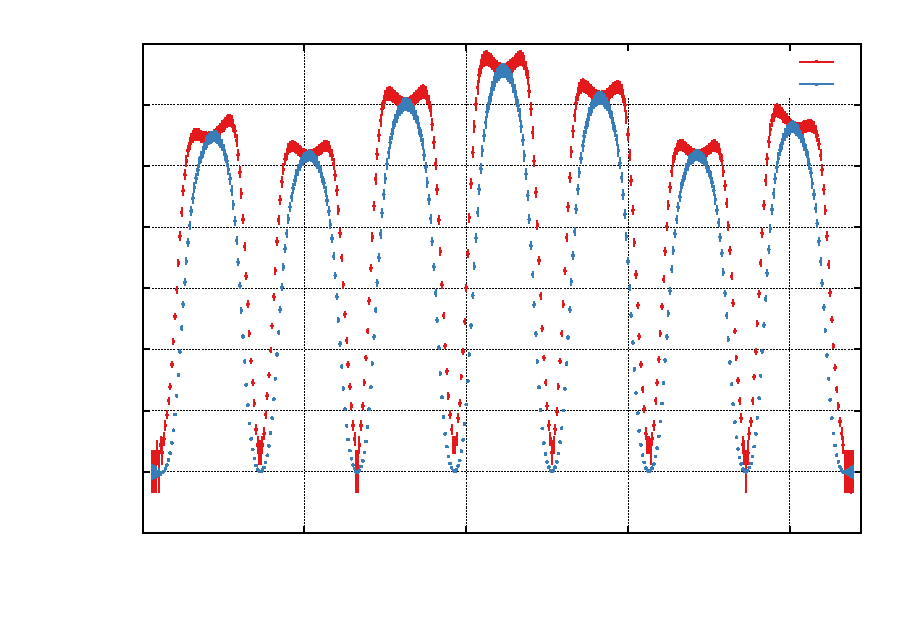
\includegraphics{./plots/PETRA-IV/pi}}%
    \gplfronttext
  \end{picture}%
\endgroup

	\caption[Elektrische Feldverteilung der $\mathrm{TM}_{010}\text{-}\pi$-Beschleunigungsmode von PETRA-III]{Elektrische Feldverteilung der $\mathrm{TM}_{010}\text{-}\pi$-Beschleunigungsmode von PETRA-III. Die Position~$z$ ist relativ zum Vakuumflansch angegeben.}
	\label{fig:bsp_feld_tm010pi_petra3}
\end{figure}

Schließlich können die charakteristischen Größen der $\mathrm{TM}_{010}$-Moden bestimmt werden, wobei die folgenden Überlegungen auf dem Inhalt von Abschnitt \ref{sec:resonator_charakteristiken} basieren.
Zunächst erfolgt die Berechnung der longitudinalen Shuntimpedanzen~$R_\mathrm{S}$, indem Gleichung \eqref{eq:beschleunigungsspannung} in \eqref{eq:shuntimpedanz} eingesetzt wird, sodass man
\begin{align}
	R_\mathrm{S} = \frac{1}{2} \left( \int_0^L \frac{|\ve_0(z)|}{\sqrt{P_\mathrm{V}}} \, \mathrm{d}z \right)^2
\end{align}
erhält.
Demnach kann die Shuntimpedanz durch Integration der (normierten) elektrischen Feldamplitude über die Länge~$L$ des Resonators gewonnen werden.
Diese Integration sowie die hierauf folgenden Integrationen erfolgen dabei numerisch durch die Trapezregel.
Ebenso kann der Laufzeitfaktor~$\Lambda$ als das Verhältnis des Integrals von effektivem Feld zum Integral der Feldamplitude berechnet werden.
Dieser dient der Berechnung der effektiven Shuntimpedanz~$R_\mathrm{S}^\mathrm{eff}$, die nun durch Gleichung \eqref{eq:eff_shuntimpedanz} bestimmt werden kann.
Alternativ kann die effektive Shuntimpedanz durch Integration über das effektive Feld, analog zur Berechnung der Shuntimpedanz, ermittelt werden.

Die Kenngrößen der verschiedenen $\mathrm{TM}_{010}$-Resonatormoden und deren longitudinalen Shuntimpedanzen wurden in Tabelle \ref{tab:shuntimpedanzen_tm010} zusammengestellt.
\begin{table}[htb]
	\begin{subtable}{1\textwidth}
		\centering
		\begin{tabular}{
		c
		S[table-format=3.2]
		S[table-format=5.0(3), table-align-uncertainty = true]
		S[table-format=2.1(3), table-align-uncertainty = true]
		S[table-format=0.3(1), table-align-uncertainty = true]
		S[table-format=3.2(2)e1, table-align-uncertainty = true]
		}
	\toprule
	{$\Delta \varphi$} & {$\nu_0$ / \si{MHz}} & {$Q_0$} & {$R_\mathrm{S}$ / \si{\mega\ohm}} & {$\Lambda$} & {$R_\mathrm{S}^\mathrm{eff}$ / \si{\ohm}} \\
	\midrule
	$\pi$ & 499.67 & 29556+-110 & 43.6+-1.6 & 0.767+-0.002 & 25.65+-0.91e6 \\[0.25em]
	$\frac{2}{3}\pi$ & 501.14 & 31741+-86 & 37.8+-1.4 & 0.092+-0.002 & 320+-11e3 \\[0.25em]
	$\frac{1}{3}\pi$ & 505.37 & 32707+-118 & 42.3+-1.5 & 0.141+-0.001 & 842+-30e3 \\[0.25em]
	$0$ & 508.61 & 35999+-66 & 46.2+-1.7 & 0.010+-0.001 & 5.0+-0.5e3 \\
	\bottomrule
\end{tabular}

		\caption{PETRA-III}
	\end{subtable}
	\begin{subtable}{1\textwidth}
		\centering
		\begin{tabular}{
		c
		S[table-format=3.2]
		S[table-format=5.0(3), table-align-uncertainty = true]
		S[table-format=2.1(3), table-align-uncertainty = true]
		S[table-format=0.3(1), table-align-uncertainty = true]
		p{-1mm}
		S[table-format=2.2]
		@{ $\pm$ }
		S[table-format= 1.2]
		@{\,) $\cdot$ }
		l
		}
	\toprule
	{$\Delta \varphi$} & {$\nu_0$ / \si{MHz}} & {$Q_0$} & {$R_\mathrm{S}$ / \si{\mega\ohm}} & {$\Lambda$} & \multicolumn{4}{c}{$R_\mathrm{S}^\mathrm{eff}$ / \si{\ohm}} \\
	\midrule
	$\pi$ & 499.67 & 28200+-176 & 41.6+-1.5 & 0.767+-0.001 & ( & 24.47 & 0.87 & $10^6$ \\[0.25em]
	$\frac{2}{3}\pi$ & 501.17 & 31356+-218 & 37.5+-1.4 & 0.056+-0.001 & ( & 115.3 & 4.1 & $10^3$ \\[0.25em]
	$\frac{1}{3}\pi$ & 505.43 & 32732+-54 & 42.3+-1.5 & 0.041+-0.001 & ( & 69.8 & 2.4 & $10^3$ \\[0.25em]
	$0$ & 508.61 & 35445+-59 & 45.4+-1.6 & 0.013+-0.001 & ( & 7.7 & 0.6 & $10^3$ \\
	\bottomrule
\end{tabular}

		\caption{PETRA-IV}
	\end{subtable}
	\caption[Longitudinale Shuntimpedanzen der $\mathrm{TM}_{010}$-Moden von PETRA-III und PETRA-IV]{Longitudinale Shuntimpedanzen der vermessenen $\mathrm{TM}_{010}$-Moden beider PETRA-Resonatoren. Die Resonanzfrequenz~$\nu_0$ wurde gemäß Abschnitt \ref{sec:vorbereitung_resonator} auf die Frequenz des evakuierten Resonators umgerechnet.}
	\label{tab:shuntimpedanzen_tm010}
\end{table}

\subsection{Vergleich und Interpretation der Ergebnisse}
Wie zu erwarten, zeigt die $\pi$-Mode beider Resonatoren mit einem Laufzeitfaktor von \SI{76,7}{\percent} die höchste effektive Shuntimpedanz.
Dies ist der Fall, da ein ultrarelativistisches Teilchen zum Durchqueren einer Zelle der Länge \SI{30}{\centi\metre} bei einer treibenden Hochfrequenz von \SI{499.67}{MHz} genau eine halbe Periode der Hochfrequenz benötigt.
Durch den Phasensprung von $\pi$ zwischen jeder Zelle bedeutet dies, dass das Teilchen stets ein elektrisches Feld erfährt, welches in dessen Bewegungsrichtung zeigt (vgl.\ Abschnitt \ref{app:tm010_felder}).
Im Vergleich dazu sind die restlichen $\mathrm{TM}_{010}$-Moden mit effektiven Shuntimpedanzen der Größenordnung von einigen \si{\kilo\ohm} ungeeignet für die effiziente Beschleunigung geladener Teilchen.
Dahingehend soll sich die Diskussion auf die $\pi$-Beschleunigungsmode beschränken.

Laut Herstellerangaben liegt die Güte der siebenzelligen PETRA-Resonatoren im Bereich von \num{29000} bis \num{36000} bei einem Nominalwert von \num{32800} \cite{desy_petra}.
PETRA-IV unterschreitet somit die Untergrenze der Güte um etwa \num{800} und lediglich PETRA-III fällt in den angegebenen Bereich.
Außerdem unterschreiten beide deutlich die nominale Güte, was möglicherweise darauf zurückzuführen ist, dass beide Resonatoren über längere Zeit belüftet waren und so eine Oxidation der Kupferoberfläche stattgefunden hat, die eine Vergrößerung der Verluste des Resonators zur Folge hat.
Im Folgenden wird diese Abweichung auch bei den Shuntimpedanzen auftreten, da diese eine lineare Abhängigkeit von der Güte der Resonatormode aufweist.

Der Hersteller gibt eine nominale (effektive) Shuntimpedanz von \SI{28.1}{\mega\ohm} an \cite{desy_petra}, welche gemäß der vorigen Erläuterungen nicht erreicht werden kann.
Ein Vergleich ist dennoch möglich, wenn der Geometriefaktor $R_\mathrm{S}^\mathrm{eff} / Q_0$ der Beschleunigungsmode betrachtet wird.
Für beide Resonatoren erhält man den Geometriefaktor der $\pi$-Mode von
\begin{align}
	\frac{R_\mathrm{S}^\mathrm{eff}}{Q_0} = \SI{868+-32}{\ohm} \eqcomma
\end{align}
welcher unabhängig von der Verlustleistung des jeweiligen Resonators ist.
Gemäß der Simulation der Kavität durch den Hersteller mit MAFIA\texttrademark\footnote{Programm zur numerischen Simulation elektromagnetischer Felder und Vorgänger des \textit{CST Microwave Studio\textsuperscript{\textregistered}}.} beträgt der Geometriefaktor \SI{856}{\ohm} \cite{desy_petra} und steht somit in guter Übereinstimmung mit den gemessenen Werten.

Wird eine treibende Hochfrequenzleistung~$P_\mathrm{HF}$ bei kritischer Kopplung (die Verlustleistung~$P_\mathrm{V}$ entspricht dann $P_\mathrm{HF}$) des Resonators angenommen, so erhält man die effektive Beschleunigungsspannung gemäß Gleichung \eqref{eq:eff_shuntimpedanz}
\begin{align}
	U_\mathrm{eff} = \sqrt{2 R_\mathrm{S}^\mathrm{eff} P_\mathrm{HF}} \eqdot
\end{align}
Wird beispielsweise zum Betrieb der Resonatoren ein $\SI{200}{\kilo\watt}$-Klystron genutzt, dessen Leistung durch ein magisches T (Leistungsteiler auf Hohlleiterbasis) gleichmäßig auf beide Resonatoren aufgeteilt wird, so erhält man effektive Beschleunigungsspannungen von
\begin{align}
	U_\mathrm{eff}^\mathrm{P-III} = \SI{2.265 +- 0.041}{\mega\volt} \qquad \text{und} \qquad U_\mathrm{eff}^\mathrm{P-IV} = \SI{2.212 +- 0.040}{\mega\volt} 
\end{align}
unter der Verwendung der gemessenen Shuntimpedanzen.
Der Vergleich mit den aktuell in \mbox{ELSA} verbauten fünfzelligen Resonatoren vom Typ PETRA mit einer effektiven Shuntimpedanz von \SI{15}{\mega\ohm} liefert bei gleicher eingekoppelter Leistung eine effektive Beschleunigungsspannung $U_\mathrm{eff} = \SI{1.73}{\mega\volt}$.
Dies zeigt eine wesentlich effizientere Beschleunigung in den siebenzelligen Resonatoren gegenüber den fünfzelligen und ist der Hauptgrund für die Konstruktion mehrzelliger Beschleunigungsresonatoren.

\section{Vermessung von Moden höherer Ordnung}
\label{sec:hom_messung}
Schließlich wurde eine Vermessung von Moden höherer Ordnung von PETRA-III durchgeführt.
Eine Vorauswahl der zu vermessenen Moden wurde dabei anhand deren Güte getroffen, so dass nur Resonanzen mit Güten der Größenordnung $10^4$ und größer in Betrachtung gezogen wurden.
Außerdem wurde ein Schwerpunkt auf die $\mathrm{TM}_{021}$-Mode bei ca. \SI{1.46}{GHz} gesetzt, da diese gemäß \cite{schedler} eine effektive Shuntimpedanz in der Größenordnung der Fundamentalmode besitzt.
Die Vermessung und Teile der Auswertung dieser Moden erfolgt analog zu Abschnitt~\ref{sec:tm010_messung} und soll daher nicht wiederholt werden.
Die Abweichungen werden im folgenden Abschnitt dargestellt.

\subsection{Auswertung der Messdaten}
Zur Auswertung der vermessenen Feldverteilungen muss zunächst die Phasenbeziehung der Felder in den einzelnen Zellen bestimmt werden.
Dazu werden Simulationen der Eigenmoden eines vereinfachten Modells des siebenzelligen PETRA-Resonators von \cite{schedler_pm} mit \textit{CST Microwave Studio\textsuperscript{\textregistered}} (CST-MWS) durchgeführt.
Aufgrund der Tatsache, dass ein vereinfachtes Modell der Kavität genutzt wird, kommt es teilweise zu großen Abweichungen der Resonanzfrequenz zwischen Simulation und Messung.
Darüber hinaus treten Diskrepanzen zwischen simulierten und gemessenen Feldamplituden auf.
Diese Abweichungen sind unter anderem auf die rudimentäre Modellierung der Nasenkegel und Abstimmstempel zurückzuführen.
Außerdem ist die Zelle der Einkopplung ohne Koppelschleife modelliert.
Dennoch ist eine Identifizierung der meisten vermessenen Resonatormoden anhand charakteristischer Merkmale der Feldverteilung zu vollziehen.
In Abbildung \ref{fig:cst_sim_tm111} wurden exemplarisch die (qualitativen) Ergebnisse einer Simulation der vermessenen $\mathrm{TM}_{111}$-Mode durch CST-MWS gezeigt. 
\begin{figure}[h]
	\centering
	\begin{subfigure}{1\textwidth}
		\centering
		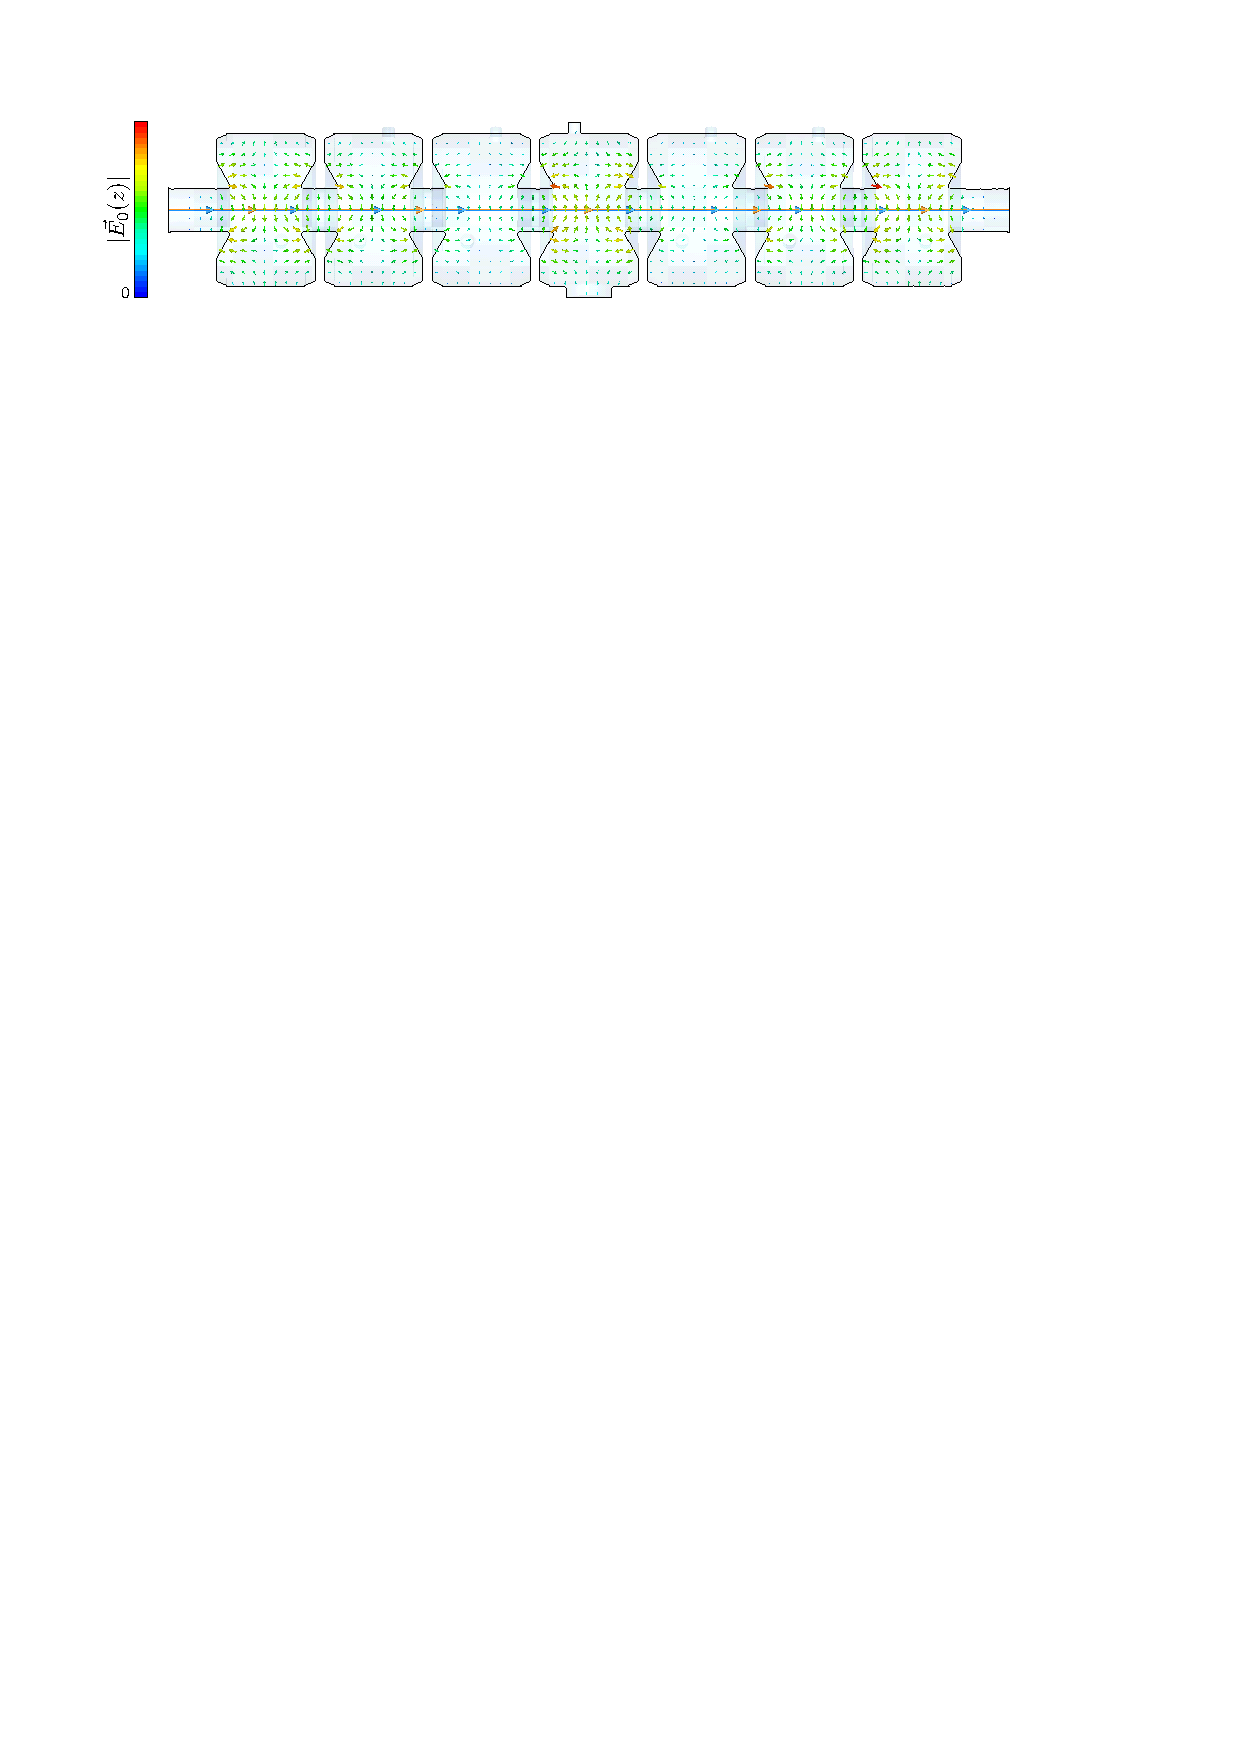
\includegraphics[width=1.0\textwidth]{./figs/TM111-CST/TM111_legende.pdf}
		\caption{Qualitative Darstellung des elektrischen Feldes zu einem festen Zeitpunkt. Gezeigt ist der Querschnitt des Resonator-Modells mit der Strahlenachse in der Schnittebene.}
	\end{subfigure}
	\begin{subfigure}{1\textwidth}
		\centering
		\hspace*{3.5mm}% GNUPLOT: LaTeX picture with Postscript
\begingroup
  \makeatletter
  \providecommand\color[2][]{%
    \GenericError{(gnuplot) \space\space\space\@spaces}{%
      Package color not loaded in conjunction with
      terminal option `colourtext'%
    }{See the gnuplot documentation for explanation.%
    }{Either use 'blacktext' in gnuplot or load the package
      color.sty in LaTeX.}%
    \renewcommand\color[2][]{}%
  }%
  \providecommand\includegraphics[2][]{%
    \GenericError{(gnuplot) \space\space\space\@spaces}{%
      Package graphicx or graphics not loaded%
    }{See the gnuplot documentation for explanation.%
    }{The gnuplot epslatex terminal needs graphicx.sty or graphics.sty.}%
    \renewcommand\includegraphics[2][]{}%
  }%
  \providecommand\rotatebox[2]{#2}%
  \@ifundefined{ifGPcolor}{%
    \newif\ifGPcolor
    \GPcolortrue
  }{}%
  \@ifundefined{ifGPblacktext}{%
    \newif\ifGPblacktext
    \GPblacktexttrue
  }{}%
  % define a \g@addto@macro without @ in the name:
  \let\gplgaddtomacro\g@addto@macro
  % define empty templates for all commands taking text:
  \gdef\gplbacktext{}%
  \gdef\gplfronttext{}%
  \makeatother
  \ifGPblacktext
    % no textcolor at all
    \def\colorrgb#1{}%
    \def\colorgray#1{}%
  \else
    % gray or color?
    \ifGPcolor
      \def\colorrgb#1{\color[rgb]{#1}}%
      \def\colorgray#1{\color[gray]{#1}}%
      \expandafter\def\csname LTw\endcsname{\color{white}}%
      \expandafter\def\csname LTb\endcsname{\color{black}}%
      \expandafter\def\csname LTa\endcsname{\color{black}}%
      \expandafter\def\csname LT0\endcsname{\color[rgb]{1,0,0}}%
      \expandafter\def\csname LT1\endcsname{\color[rgb]{0,1,0}}%
      \expandafter\def\csname LT2\endcsname{\color[rgb]{0,0,1}}%
      \expandafter\def\csname LT3\endcsname{\color[rgb]{1,0,1}}%
      \expandafter\def\csname LT4\endcsname{\color[rgb]{0,1,1}}%
      \expandafter\def\csname LT5\endcsname{\color[rgb]{1,1,0}}%
      \expandafter\def\csname LT6\endcsname{\color[rgb]{0,0,0}}%
      \expandafter\def\csname LT7\endcsname{\color[rgb]{1,0.3,0}}%
      \expandafter\def\csname LT8\endcsname{\color[rgb]{0.5,0.5,0.5}}%
    \else
      % gray
      \def\colorrgb#1{\color{black}}%
      \def\colorgray#1{\color[gray]{#1}}%
      \expandafter\def\csname LTw\endcsname{\color{white}}%
      \expandafter\def\csname LTb\endcsname{\color{black}}%
      \expandafter\def\csname LTa\endcsname{\color{black}}%
      \expandafter\def\csname LT0\endcsname{\color{black}}%
      \expandafter\def\csname LT1\endcsname{\color{black}}%
      \expandafter\def\csname LT2\endcsname{\color{black}}%
      \expandafter\def\csname LT3\endcsname{\color{black}}%
      \expandafter\def\csname LT4\endcsname{\color{black}}%
      \expandafter\def\csname LT5\endcsname{\color{black}}%
      \expandafter\def\csname LT6\endcsname{\color{black}}%
      \expandafter\def\csname LT7\endcsname{\color{black}}%
      \expandafter\def\csname LT8\endcsname{\color{black}}%
    \fi
  \fi
    \setlength{\unitlength}{0.0500bp}%
    \ifx\gptboxheight\undefined%
      \newlength{\gptboxheight}%
      \newlength{\gptboxwidth}%
      \newsavebox{\gptboxtext}%
    \fi%
    \setlength{\fboxrule}{0.5pt}%
    \setlength{\fboxsep}{1pt}%
\begin{picture}(6802.00,2834.00)%
    \gplgaddtomacro\gplbacktext{%
      \csname LTb\endcsname%
      \put(682,704){\makebox(0,0)[r]{\strut{}0}}%
      \put(682,1077){\makebox(0,0)[r]{\strut{}2}}%
      \put(682,1450){\makebox(0,0)[r]{\strut{}4}}%
      \put(682,1823){\makebox(0,0)[r]{\strut{}6}}%
      \put(682,2196){\makebox(0,0)[r]{\strut{}8}}%
      \put(682,2569){\makebox(0,0)[r]{\strut{}10}}%
      \put(814,484){\makebox(0,0){\strut{}0}}%
      \put(2073,484){\makebox(0,0){\strut{}500}}%
      \put(3332,484){\makebox(0,0){\strut{}1000}}%
      \put(4592,484){\makebox(0,0){\strut{}1500}}%
      \put(5851,484){\makebox(0,0){\strut{}2000}}%
    }%
    \gplgaddtomacro\gplfronttext{%
      \csname LTb\endcsname%
      \put(176,1636){\rotatebox{-270}{\makebox(0,0){\strut{}$|\vec{E}_0(z)|$ / willk.\ Einh.}}}%
      \put(3609,154){\makebox(0,0){\strut{}$z$ / \si{mm}}}%
    }%
    \gplbacktext
    \put(0,0){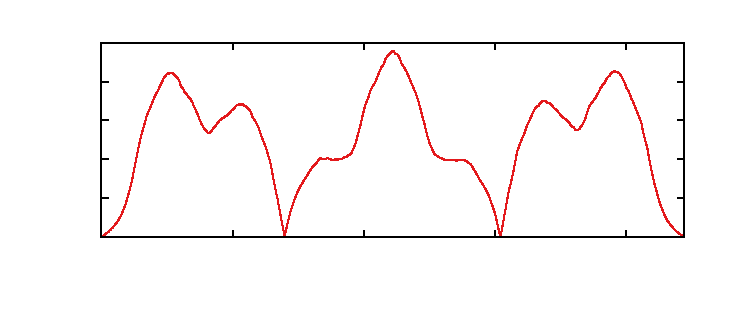
\includegraphics{./plots/tm111_abs_sim}}%
    \gplfronttext
  \end{picture}%
\endgroup

		\caption{Amplitude des elektrischen Feldes in Abhängigkeit der Position auf der Strahlenachse.}
	\end{subfigure}
	\caption[Simulation der $\mathrm{TM}_{111}$-Eigenmode des PETRA-Resonators durch CST-MWS]{Simulation der vermessenen $\mathrm{TM}_{111}$-Eigenmode durch CST-MWS.}
	\label{fig:cst_sim_tm111}
\end{figure}
Ein wichtiges Merkmal ist das Verschwinden des elektrischen Feldes zwischen Zellen mit einem Phasensprung des elektrischen Feldes von $\pi$.
Dies ist zwischen der zweiten und dritten Zelle in Abbildung \ref{fig:cst_sim_tm111} zu beobachten und kann zur eindeutigen Identifikation der meisten Resonatormoden und deren Phasenbeziehung genutzt werden.

Für zwei der vermessenen Moden ist keine eindeutige Bestimmung der Phasenbeziehung zu vollziehen, da diese keinen Eigenmoden der Simulation durch CST-MWS zugeordnet werden können.
Außerdem ist eine Festlegung der Phasenbeziehung durch das zuvor erwähnte Merkmal nicht möglich, da die betroffenen Moden eine verschwindende elektrische Feldamplitude in den mittleren Zellen aufweisen (vgl.\ Abb.\ \ref{fig:tm021_1458} f.).
Daher wird für diese Moden die Phasenbeziehung so gewählt, dass der Fall maximaler effektiver Shuntimpedanz eintritt.

Für Moden höherer Ordnung können gemäß Abschnitt \ref{sec:em_felder_in_resonatoren} auch $\pi$-Phasensprünge innerhalb einer Zelle stattfinden (z.\ B.\ bei den $\mathrm{TM}_{021}$-Moden), welche ebenfalls bei der Auswertung beachtet werden müssen.

Die restliche Auswertung folgt analog zu Abschnitt \ref{sec:tm010_messung} und die Ergebnisse wurden in Tabelle~\ref{tab:shuntimpedanzen_hom} dargestellt.
Die Darstellungen der elektrischen Felder wurde in Abschnitt~\ref{app:hom_felder} zusammengefasst.
\begin{table}[htb]
	\centering
	\begin{tabular}{
		c
		c
		S[table-format=4.2]
		S[table-format=5.0(3), table-align-uncertainty = true]
		S[table-format=1.3(3), table-align-uncertainty = true]
		S[table-format=0.3(1), table-align-uncertainty = true]
		S[table-format=3.2(2), table-align-uncertainty = true]
		}
	\toprule
	\multicolumn{2}{c}{Mode} & {$\nu_0$ / \si{MHz}} & {$Q_0$} & {$R_\mathrm{S}$ / \si{\mega\ohm}} & {$\Lambda$} & {$R_\mathrm{S}^\mathrm{eff}$ / \si{\kilo\ohm}} \\
	\midrule
	$\mathrm{TE}_{111}$ & trans. & 702.70 & 11162+-18 & 3.89+-0.14 & 0.289+-0.002 & 326+-11 \\[0.25em]
	$\mathrm{TM}_{011}$ & long. & 730.45 & 13927+-39 & 3.28+-0.12 & 0.118+-0.003 & 45.8+-1.6 \\[0.25em]
	$\mathrm{TM}_{111}$ & trans. & 1047.23 & 28528+-174 & 8.14+-0.29 & 0.017+-0.001 & 2.34+-0.15 \\[0.25em]
	---\textsuperscript{\textasteriskcentered} & long. & 1375.79 & 59762+-416 & 9.47+-0.34 & 0.019+-0.002 & 3.40+-0.40 \\[0.25em]
	$\mathrm{TM}_{021}$\textsuperscript{\textdagger} & long. & 1458.30 & 7552+-51 & 0.566+-0.020 & 0.182+-0.004 & 18.8+-0.7 \\[0.25em]
	$\mathrm{TM}_{021}$\textsuperscript{\textdagger} & long. & 1460.34 & 16043+-63 & 0.729+-0.026 & 0.266+-0.004 & 51.7+-1.8 \\[0.25em]
	$\mathrm{TM}_{021}$ & long. & 1464.96 & 25279+-172 & 2.60+-0.10 & 0.100+-0.002 & 26.1+-1.0 \\[0.25em]
	$\mathrm{TM}_{021}$ & long. & 1465.83 & 15028+-92 & 2.52+-0.09 & 0.269+-0.001 & 183.0+-6.4 \\
	\midrule
	\multicolumn{7}{l}{
		\small{\textsuperscript{\textasteriskcentered}: Nicht Klassifizierbar nach zylindrischen Hohlräumen}
	}\\
	\multicolumn{7}{l}{
		\small{\textsuperscript{\textdagger}: Für Phasenbeziehung wurde worst-case angenommen}
	}\\
	\bottomrule
\end{tabular}

	\caption[Longitudinale/Transversale Shuntimpedanzen der Moden höherer Ordnung von PETRA-III]{Longitudinale/Transversale Shuntimpedanzen der vermessenen Moden höherer Ordnung von PETRA-III. Die Resonanzfrequenz $\nu_0$ wurde gemäß Abschnitt \ref{sec:vorbereitung_resonator} auf die Frequenz des evakuierten Resonators umgerechnet.}
	\label{tab:shuntimpedanzen_hom}
\end{table}


\subsection{Interpretation der Ergebnisse}
Bevor eine Diskussion der resultierenden Shuntimpedanzen erfolgt, sollen die gemessenen Verteilungen des elektrischen Feldes erörtert werden.
Einerseits fällt bei Betrachtung der Feldverteilungen in Abschnitt \ref{app:hom_felder} auf, dass Sprünge des effektiven elektrischen Feldes auftreten.
Diese entstehen an Stellen, an denen das elektrische Feld einen Phasensprung vollzieht und ist auf die begrenzte Ortsauflösung durch die Ausdehnung des verwendeten Störkörpers zurückzuführen.
%Dies ist der Fall, da an solchen Stellen ein Knoten der elektrischen Feldstärke vorliegt, welcher bei der Störkörpermessung nicht als solcher erscheint, da aufgrund der Ausdehnung des Störkörpers eine Frequenzverschiebung durch die umliegenden Stellen nicht-verschwindender Amplitude zu einer Frequenzverschiebung führen.
Bei der Bestimmung der Shuntimpedanzen durch Integration stellen diese Sprungstellen jedoch keinen signifikanten Einfluss dar und können vernachlässigt werden.
Mit der Verwendung eines kleineren Störkörpers wäre dennoch eine Möglichkeit gegeben, diese Sprünge zu vermindern, was jedoch mit einer Abnahme der Frequenzverschiebung durch die Störung der Resonatormoden zusammenhängen würde.
Insbesondere bei den Moden höherer Ordnung, die im Vergleich zur Fundamentalmode kleine Feldstärken aufweisen, kann dies eine Temperaturstabilisierung von Resonator und VNA erfordern und wurde daher nicht ausgenutzt.

Ferner führt die über den Messbereich konstante Frequenzauflösung des VNA und die Proportionalität
\begin{align}
\frac{|\ve_0|}{\sqrt{P_\mathrm{V}}} \propto \sqrt{\Delta \omega}
\end{align}
aus Gl.\ \eqref{eq:skm_e_feld_normiert} zu einer Abnahme der Auflösung, mit der die Amplitude des elektrischen Feldes gemessen werden kann, bei kleinen Amplituden des Feldes.
Dies führt dazu, dass Feldamplituden, die unter die Auflösungsgrenze fallen, nicht von einem verschwindenden elektrischen Feld zu unterscheiden sind.
Dadurch kann an manche Moden mit scheinbar verschwindendem elektrischen Feld (und damit auch magnetischem Feld) in der mittleren Resonatorzelle (vgl.\ Abb.\ \ref{fig:tm021_1458} ff.) eine Kopplung stattfinden.

Generell zeigen die meisten vermessenen Moden eine Shuntimpedanz~$R_\mathrm{S}^\mathrm{eff}$ von einigen \si{\mega\ohm}.
Jedoch führen die kleinen Laufzeitfaktoren~$\Lambda$ gemäß Gl.\ \eqref{eq:eff_shuntimpedanz} zu einer Reduzierung der effektiven Shuntimpedanz um den Faktor $\Lambda^2$.
Dies resultiert darin, dass die effektiven Shuntimpedanzen Werte in der Größenordnung von einigen \si{\kilo\ohm} annehmen.
Die größte effektive Shuntimpedanz zeigt dabei die $\mathrm{TE_{111}}$-Mode mit $\SI{326 +- 11}{\kilo\ohm}$ (transversal).
Der Vergleich mit der effektiven Shuntimpedanz der Fundamentalmode von etwa \SI{25}{\mega\ohm} zeigt bereits, dass der parasitäre Einfluss dieser Mode gegenüber der Fundamentalmode klein ist.
Darüber hinaus zeigt die Mode mit der Resonanzfrequenz \SI{1465.83}{MHz} die größte effektive Shuntimpedanz der $\mathrm{TM}_{021}$-Moden.
Diese liegt bei \SI{183.0 +- 6.4}{\kilo\ohm} und fällt damit ebenfalls zwei Größenordnungen unter die effektive Shuntimpedanz der Fundamentalmode.

Abschließend ist zu bemerken, dass entgegen der Erwartung keine der vermessenen Moden höherer Ordnung effektive Shuntimpedanzen in der Größenordnung der Fundamentalmode aufweist.
Dennoch ist anzumerken, dass die Untersuchung dieser Moden keineswegs umfassend war, da eine unendliche Anzahl von Moden höherer Ordnung existieren.
Bei einer weitergehenden Analyse ist eine Simulation des Impedanzspektrums (z.\ B.\ durch \textit{CST Particle Studio\textsuperscript{\textregistered}}) unter Verwendung eines detaillierteren Modells des Resonators zweckmäßig, da dadurch eine bessere Identifizierung der kritischen Moden vollzogen werden kann.
Außerdem kann dadurch eine Untersuchung des Einflusses von Moden höherer Ordnung auf Multi-Bunch-Instabilitäten an ELSA durchgeführt werden.

%==============================================================================
\chapter{Zusammenfassung und Ausblick}
\label{sec:fazit}
%==============================================================================
Im Rahmen dieser Arbeit wurde die Methode der resonanten Störkörpermessung zur Bestimmung der elektrischen Felder in Hohlraumresonatoren vorgestellt.
Dazu wurde ein Störkörpermessstand aufgebaut und um die Möglichkeit einer Störkörpermessung ohne Temperaturstabilisierung des Resonators erweitert.
Diese Messmethode wurde an zwei siebenzelligen Resonatoren vom Typ PETRA erfolgreich erprobt, indem eine Vermessung der elektrischen Felder der $\mathrm{TM}_{010}$-Resonatormode und einiger Moden höherer Ordnung erfolgte.

Die Vermessung der Fundamentalmode beider Resonatoren ergab effektive Shuntimpedanzen von etwa \SI{25}{\mega\ohm} und überschreitet somit die Erwartungen von \SI{23}{\mega\ohm} in \cite{schedler}.
Demnach sollten beide Resonatoren vom Standpunkt der Beschleunigungsspannung uneingeschränkt bei der Erweiterung von ELSA zum Einsatz kommen können.

Außerdem wurde eine Vermessung von einigen Moden höherer Ordnung durchgeführt und deren Shuntimpedanzen bestimmt.
Alle effektiven Shuntimpedanzen der vemessenen Moden höherer Ordnung liegen mehrere Größenordnungen unter der effektiven Shuntimpedanz der Fundamentalmode und stellen keine große Gefahr für die Anregung von Multi-Bunch-Instabilitäten dar.
Da keine umfassende Vermessung aller Moden höherer Ordnung durchgeführt wurde, kann der Zusammenhang von weiteren Moden mit Multi-Bunch-Instabilitäten an ELSA eine Grundlage für zukünftige Untersuchungen darstellen.


% Uncomment the following command to get references per chapter.
% Put it inside the file or change \include to \input if you do not want the references
% on a separate page
% \printbibliography[heading=subbibliography]

%------------------------------------------------------------------------------
\appendix
% \part*{Appendix}
%
% Add your appendices here - don't forget to also add them to \includeonly above
%------------------------------------------------------------------------------
\chapter{>>>Theorie<<<}
\label{sec:appendix}
%------------------------------------------------------------------------------


%------------------------------------------------------------------------------
\section{Herleitung der Frequenzverschiebung bei Störkörpermessung}
\label{app:herleitung_frequenzverschiebung}
%------------------------------------------------------------------------------
Man betrachte das zeit- und ortsabhängige elektromagnetische Feld in einem Hohlraumresonators, charakterisiert durch elektrische Feldstärke~$\ve$ und magnetische Feldstärke~$\vh$.
Die Felder des ungestörten Resonators seien gegeben durch $(\ve_0, \vh_0)$ und die des gestörten Resonators durch $(\ve_1, \vh_1)$.
Bei Verwendung der komplexen Darstellung der stehenden Welle im Resonator, kann das elektromagnetische Feld angegeben werden als:
\begin{subequations}
  \label{eq:skm_felder}
  \begin{align}
  &\ve_{0,1}(x,y,z,t) = \ve_{0,1}(x,y,z) \, \E^{\I \omega_{0,1} t}\\
  &\vh_{0,1}(x,y,z,t) = \vh_{0,1}(x,y,z) \, \E^{\I \omega_{0,1} t}
  \end{align}
\end{subequations}
wobei die Phasenbeziehung von elektrischem und magnetischem Feld in den komplexen Amplituden $\ve_{0,1}(x,y,z)$ und $\vh_{0,1}(x,y,z)$. enthalten ist.
Unabhängig von der Störung des Feldes gelten die \textsc{Maxwell}-Gleichungen \cite{jackson}:
\begin{subequations}
  \label{eq:skm_maxwell}
  \begin{align}
    \vnabla \times \ve &= - \frac{\partial \vb}{\partial t}\\
    \vnabla \times \vh &= \vec{j}_\mathrm{frei} + \frac{\partial \vd}{\partial t}
  \end{align}
\end{subequations}
Setzt man die gestörten und ungestörten Felder \eqref{eq:skm_felder} in die \textsc{Maxwell}-Gleichung \eqref{eq:skm_maxwell} ein, so erhält man unter der Annahme einer verschwindenden freien Stromdichte $\vec{j}_\mathrm{frei}$ im Hohlraum und nach Elimination der Zeitabhängigkeit:
\begin{subequations}
  \label{eq:skm_zeitunabhaengig}
  \begin{align}
    &\vnabla \times \ve_{0,1} = - \I \omega_{0,1} \vb_{0,1} \\
    &\vnabla \times \vh_{0,1} = \I \omega_{0,1} \vd_{0,1}
  \end{align}
\end{subequations}
Man verwendet diese zeitunabhängigen Gleichungen und die Produktregel der Divergenz für das Kreuzprodukt um die folgenden Identitäten zu finden:
\begin{subequations}
  \label{eq:skm_vektoridentitaeten}
  \begin{align}
  \vnabla \cdot \left( \ve_0^* \times \vh_1\right) &= \vh_1 \cdot \left( \vnabla \times \ve_0^* \right) - \ve_0^* \cdot \left( \vnabla \times \vh_1 \right) \nonumber \\
  &= \I \omega_0 \vb_0^* \vh_1 - \I \omega_1 \ve_0^* \vd_1 \label{eq:e0h1} \\[0.5em]
  %
  \vnabla \cdot \left( \ve_1 \times \vh_0^* \right) &= \vh_0^* \cdot \left( \vnabla \times \ve_1 \right) - \ve_1 \cdot \left( \vnabla \times \vh_0^* \right) \nonumber \\
  &= \I \omega_0 \ve_1 \vd_0^* - \I \omega_1 \vb_1 \vh_0^* \label{eq:e1h0}
  \end{align}
\end{subequations}
Anschließend bildet man die Summe der Gleichungen \eqref{eq:skm_vektoridentitaeten} und führt eine Integration über das Resonatorvolumen $V$ durch.
Unter Verwendung des \textsc{Gauß}schen Integralsatzes erhält man:
\begin{align}
  \int_{V} \mathrm{d}V \left[ \vnabla \cdot \left( \ve_0^* \times \vh_1 + \ve_1 \times \vh_0^* \right) \right] = \oint_{\partial V} \mathrm{d}S \left[ \vec{n} \cdot \left( \ve_0^* \times \vh_1 + \ve_1 \times \vh_0^* \right)\right] \label{eq:volint}
\end{align}
wobei $\vec{n}$ den Normaleneinheitsvektor auf dem Rand $\partial V$ des Resonatorhohlraums darstellt.
Die Randbedingungen für das elektrische und magnetische Feld am idealen Leiter \eqref{eq:randbedingung_leiter} sorgen dafür, dass das Skalarprodukt im Integranden der rechten Seite auf dem Rand des Volumens $\partial V$ identisch verschwindet\footnote{Das Kreuzprodukt von elektrischer und magnetischer Feldstärke steht stehts senkrecht zum Normalenvektor der ideal leitenden Grenzfläche: $\ve \times \vh \perp \vec{n}$}.
Setzt man die gefundenen Identitäten \eqref{eq:skm_vektoridentitaeten} in das Integral über das Resonatorvolumen ein, so erhält den Zusammenhang zwischen ungestörter~$\omega_0$ und gestörter Resonanzfrequenz~$\omega_1$:
\begin{align}
  \omega_0 \int_{V} \mathrm{d}V \left( \vb_0^* \cdot \vh_1 + \ve_1 \cdot \vd_0^* \right) = \omega_1 \int_{V} \mathrm{d}V \left( \vb_1 \cdot \vh_0^* + \ve_0^* \cdot \vd_1 \right)
\end{align}
Dieser Zusammenhang ermöglicht es einen Ausdruck ermöglicht die Angabe der relativen Frequenzverschiebung:
\begin{align}
  \frac{\Delta \omega}{\omega_0}= \frac{\omega_1 - \omega_0}{\omega_0} = \frac{\int_{V} \mathrm{d}V \left[ \left( \ve_1 \cdot \vd_0^* - \ve_0^* \cdot \vd_1 \right) + \left( \vb_0^* \cdot \vh_1 - \vb_1 \cdot \vh_0^* \right)\right]}{\int_V \mathrm{d}V \left[\ve_0^* \cdot \vd_1 + \vb_1 \cdot \vh_0^* \right] }
  \label{eq:skm_rel_freqabweichung_schritt}
\end{align}
Unter Verwendung der Definitionen für die magnetische Feldstärke $\vh$ und der elektrischen Flussdichte $\vd$:
\begin{subequations}
  \begin{align}
    &\vd \coloneqq \epsilon_0 \ve + \vec{P}\\
    &\vh \coloneqq \frac{1}{\mu_0} \vb - \vec{M}
  \end{align}
\end{subequations}
mit den Vektorfeldern der Polarisation $\vec{P}$ und Magnetisierung $\vec{M}$ folgt aus \eqref{eq:skm_rel_freqabweichung_schritt}:
\begin{align}
  \frac{\Delta \omega}{\omega_0} = - \frac{\int_V \mathrm{d}V \left[ \ve_0^* \cdot \vec{P} + \vb_0^* \cdot \vec{M} \right]}{\int_V \mathrm{d}V \left[ \ve_0^* \cdot \vd_1 + \vb_1 \cdot \vh_0^* \right]} \label{eq:skm_rel_freqabweichung_schritt2}
\end{align}
Schließlich wird angenommen, dass das Volumen des Störkörpers klein ist gegen das gesamte Resonatorvolumen.
Dadurch können bei Integration über das Resonatorvolumen im Nenner von \eqref{eq:skm_rel_freqabweichung_schritt2}, die gestörten Felder im Integranden durch die Ungestörten genähert werden.
Beachtet man weiterhin, dass die Phasendifferenz von elektrischem und magnetischem Feld bei stehenden elektromagnetischen Wellen $\pi / 2$ beträgt, so erhält man nach Ausführen der Integration im Nenner die vierfache im Feld des Resonators gespeicherte Energie~$W_0$:
\begin{align}
  \frac{\Delta \omega}{\omega_0} = - \frac{\int_V \mathrm{d}V \left[ \ve_0^* \cdot \vec{P} + \vb_0^* \cdot \vec{M} \right]}{4 W_0}
\end{align}
Diese Gleichung verknüpft die Verschiebung der Resonanzfrequenz durch einen Störkörper mit den ungestörten elektrischen und magnetischen Feldern und ermöglicht die Messung der Felder bei geeigneter Wahl des Störkörpers.
\todo{Frequenzverschiebung ist negativ}

%------------------------------------------------------------------------------
\chapter{Ergebnisse der Störkörpermessungen}
\label{sec:appendix_felder}
%------------------------------------------------------------------------------

%------------------------------------------------------------------------------
\section{Elektrische Feldverteilung der $\mathrm{TM}_{010}$-Resonatormoden}
\label{app:tm010_felder}
%------------------------------------------------------------------------------
Im Folgenden werden die Feldverteilungen der vermessenen $\mathrm{TM}_{010}$-Resonatormoden der beiden Resonatoren PETRA-III und PETRA-IV zusammengetragen.
In allen Fällen ist die Position~$z$ relativ zum Vakuumflansch des Resonators und die elektrischen Felder normiert auf die Wurzel der Verlustleistung~$P_\mathrm{V}$ angegeben.

\subsection{PETRA-III}
\FloatBarrier
\begin{figure}[h]
  \centering
  % GNUPLOT: LaTeX picture with Postscript
\begingroup
  \makeatletter
  \providecommand\color[2][]{%
    \GenericError{(gnuplot) \space\space\space\@spaces}{%
      Package color not loaded in conjunction with
      terminal option `colourtext'%
    }{See the gnuplot documentation for explanation.%
    }{Either use 'blacktext' in gnuplot or load the package
      color.sty in LaTeX.}%
    \renewcommand\color[2][]{}%
  }%
  \providecommand\includegraphics[2][]{%
    \GenericError{(gnuplot) \space\space\space\@spaces}{%
      Package graphicx or graphics not loaded%
    }{See the gnuplot documentation for explanation.%
    }{The gnuplot epslatex terminal needs graphicx.sty or graphics.sty.}%
    \renewcommand\includegraphics[2][]{}%
  }%
  \providecommand\rotatebox[2]{#2}%
  \@ifundefined{ifGPcolor}{%
    \newif\ifGPcolor
    \GPcolortrue
  }{}%
  \@ifundefined{ifGPblacktext}{%
    \newif\ifGPblacktext
    \GPblacktexttrue
  }{}%
  % define a \g@addto@macro without @ in the name:
  \let\gplgaddtomacro\g@addto@macro
  % define empty templates for all commands taking text:
  \gdef\gplbacktext{}%
  \gdef\gplfronttext{}%
  \makeatother
  \ifGPblacktext
    % no textcolor at all
    \def\colorrgb#1{}%
    \def\colorgray#1{}%
  \else
    % gray or color?
    \ifGPcolor
      \def\colorrgb#1{\color[rgb]{#1}}%
      \def\colorgray#1{\color[gray]{#1}}%
      \expandafter\def\csname LTw\endcsname{\color{white}}%
      \expandafter\def\csname LTb\endcsname{\color{black}}%
      \expandafter\def\csname LTa\endcsname{\color{black}}%
      \expandafter\def\csname LT0\endcsname{\color[rgb]{1,0,0}}%
      \expandafter\def\csname LT1\endcsname{\color[rgb]{0,1,0}}%
      \expandafter\def\csname LT2\endcsname{\color[rgb]{0,0,1}}%
      \expandafter\def\csname LT3\endcsname{\color[rgb]{1,0,1}}%
      \expandafter\def\csname LT4\endcsname{\color[rgb]{0,1,1}}%
      \expandafter\def\csname LT5\endcsname{\color[rgb]{1,1,0}}%
      \expandafter\def\csname LT6\endcsname{\color[rgb]{0,0,0}}%
      \expandafter\def\csname LT7\endcsname{\color[rgb]{1,0.3,0}}%
      \expandafter\def\csname LT8\endcsname{\color[rgb]{0.5,0.5,0.5}}%
    \else
      % gray
      \def\colorrgb#1{\color{black}}%
      \def\colorgray#1{\color[gray]{#1}}%
      \expandafter\def\csname LTw\endcsname{\color{white}}%
      \expandafter\def\csname LTb\endcsname{\color{black}}%
      \expandafter\def\csname LTa\endcsname{\color{black}}%
      \expandafter\def\csname LT0\endcsname{\color{black}}%
      \expandafter\def\csname LT1\endcsname{\color{black}}%
      \expandafter\def\csname LT2\endcsname{\color{black}}%
      \expandafter\def\csname LT3\endcsname{\color{black}}%
      \expandafter\def\csname LT4\endcsname{\color{black}}%
      \expandafter\def\csname LT5\endcsname{\color{black}}%
      \expandafter\def\csname LT6\endcsname{\color{black}}%
      \expandafter\def\csname LT7\endcsname{\color{black}}%
      \expandafter\def\csname LT8\endcsname{\color{black}}%
    \fi
  \fi
    \setlength{\unitlength}{0.0500bp}%
    \ifx\gptboxheight\undefined%
      \newlength{\gptboxheight}%
      \newlength{\gptboxwidth}%
      \newsavebox{\gptboxtext}%
    \fi%
    \setlength{\fboxrule}{0.5pt}%
    \setlength{\fboxsep}{1pt}%
\begin{picture}(8502.00,5668.00)%
    \gplgaddtomacro\gplbacktext{%
      \csname LTb\endcsname%
      \put(1078,704){\makebox(0,0)[r]{\strut{}-1000}}%
      \csname LTb\endcsname%
      \put(1078,1291){\makebox(0,0)[r]{\strut{}0}}%
      \csname LTb\endcsname%
      \put(1078,1879){\makebox(0,0)[r]{\strut{}1000}}%
      \csname LTb\endcsname%
      \put(1078,2466){\makebox(0,0)[r]{\strut{}2000}}%
      \csname LTb\endcsname%
      \put(1078,3054){\makebox(0,0)[r]{\strut{}3000}}%
      \csname LTb\endcsname%
      \put(1078,3641){\makebox(0,0)[r]{\strut{}4000}}%
      \csname LTb\endcsname%
      \put(1078,4228){\makebox(0,0)[r]{\strut{}5000}}%
      \csname LTb\endcsname%
      \put(1078,4816){\makebox(0,0)[r]{\strut{}6000}}%
      \csname LTb\endcsname%
      \put(1078,5403){\makebox(0,0)[r]{\strut{}7000}}%
      \csname LTb\endcsname%
      \put(1210,484){\makebox(0,0){\strut{}0}}%
      \csname LTb\endcsname%
      \put(2763,484){\makebox(0,0){\strut{}500}}%
      \csname LTb\endcsname%
      \put(4316,484){\makebox(0,0){\strut{}1000}}%
      \csname LTb\endcsname%
      \put(5869,484){\makebox(0,0){\strut{}1500}}%
      \csname LTb\endcsname%
      \put(7422,484){\makebox(0,0){\strut{}2000}}%
    }%
    \gplgaddtomacro\gplfronttext{%
      \csname LTb\endcsname%
      \put(176,3053){\rotatebox{-270}{\makebox(0,0){\strut{}$\frac{E_0(z)}{\sqrt{P_\mathrm{V}}}$ / \si{\volt\per\metre\per\watt\tothe{0{,}5}}}}}%
      \put(4657,154){\makebox(0,0){\strut{}$z$ / \si{mm}}}%
      \csname LTb\endcsname%
      \put(7382,5230){\makebox(0,0)[r]{\strut{}Amplitude}}%
      \csname LTb\endcsname%
      \put(7382,5010){\makebox(0,0)[r]{\strut{}effektives Feld}}%
    }%
    \gplbacktext
    \put(0,0){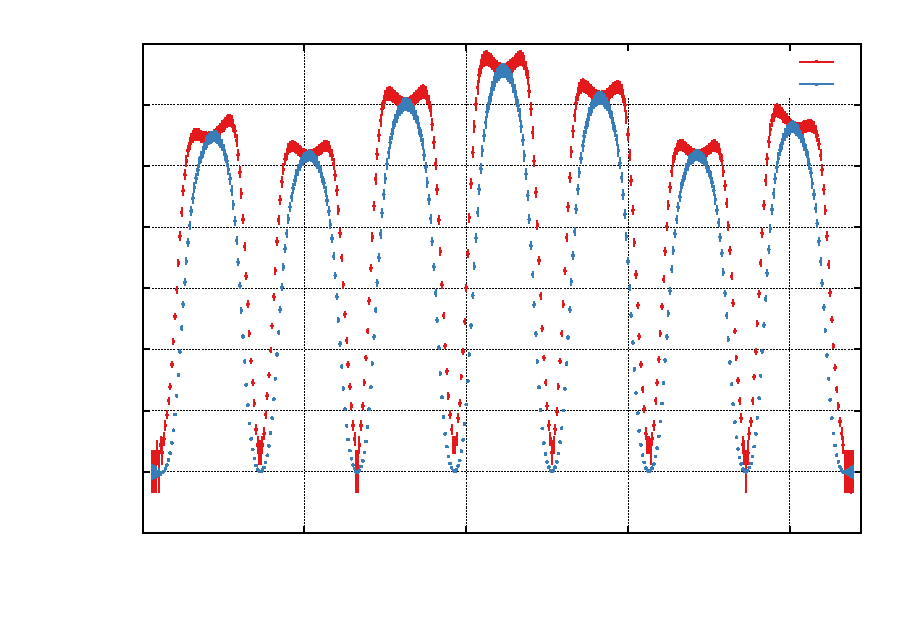
\includegraphics{./plots/PETRA-IV/pi}}%
    \gplfronttext
  \end{picture}%
\endgroup

  \caption[Feldverteilung der $\mathrm{TM}_{010}\text{-}\pi$-Mode von PETRA-III]{Verteilung des longitudinalen elektrischen Feldes der $\mathrm{TM}_{010}\text{-}\pi$-Mode von PETRA-III bei einer Resonanzfrequenz von \mbox{$\nu_0 = \SI{499.67}{MHz}$} im Vakuum.}
\end{figure}

\begin{figure}[p]
	\centering
	
	% GNUPLOT: LaTeX picture with Postscript
\begingroup
  \makeatletter
  \providecommand\color[2][]{%
    \GenericError{(gnuplot) \space\space\space\@spaces}{%
      Package color not loaded in conjunction with
      terminal option `colourtext'%
    }{See the gnuplot documentation for explanation.%
    }{Either use 'blacktext' in gnuplot or load the package
      color.sty in LaTeX.}%
    \renewcommand\color[2][]{}%
  }%
  \providecommand\includegraphics[2][]{%
    \GenericError{(gnuplot) \space\space\space\@spaces}{%
      Package graphicx or graphics not loaded%
    }{See the gnuplot documentation for explanation.%
    }{The gnuplot epslatex terminal needs graphicx.sty or graphics.sty.}%
    \renewcommand\includegraphics[2][]{}%
  }%
  \providecommand\rotatebox[2]{#2}%
  \@ifundefined{ifGPcolor}{%
    \newif\ifGPcolor
    \GPcolortrue
  }{}%
  \@ifundefined{ifGPblacktext}{%
    \newif\ifGPblacktext
    \GPblacktexttrue
  }{}%
  % define a \g@addto@macro without @ in the name:
  \let\gplgaddtomacro\g@addto@macro
  % define empty templates for all commands taking text:
  \gdef\gplbacktext{}%
  \gdef\gplfronttext{}%
  \makeatother
  \ifGPblacktext
    % no textcolor at all
    \def\colorrgb#1{}%
    \def\colorgray#1{}%
  \else
    % gray or color?
    \ifGPcolor
      \def\colorrgb#1{\color[rgb]{#1}}%
      \def\colorgray#1{\color[gray]{#1}}%
      \expandafter\def\csname LTw\endcsname{\color{white}}%
      \expandafter\def\csname LTb\endcsname{\color{black}}%
      \expandafter\def\csname LTa\endcsname{\color{black}}%
      \expandafter\def\csname LT0\endcsname{\color[rgb]{1,0,0}}%
      \expandafter\def\csname LT1\endcsname{\color[rgb]{0,1,0}}%
      \expandafter\def\csname LT2\endcsname{\color[rgb]{0,0,1}}%
      \expandafter\def\csname LT3\endcsname{\color[rgb]{1,0,1}}%
      \expandafter\def\csname LT4\endcsname{\color[rgb]{0,1,1}}%
      \expandafter\def\csname LT5\endcsname{\color[rgb]{1,1,0}}%
      \expandafter\def\csname LT6\endcsname{\color[rgb]{0,0,0}}%
      \expandafter\def\csname LT7\endcsname{\color[rgb]{1,0.3,0}}%
      \expandafter\def\csname LT8\endcsname{\color[rgb]{0.5,0.5,0.5}}%
    \else
      % gray
      \def\colorrgb#1{\color{black}}%
      \def\colorgray#1{\color[gray]{#1}}%
      \expandafter\def\csname LTw\endcsname{\color{white}}%
      \expandafter\def\csname LTb\endcsname{\color{black}}%
      \expandafter\def\csname LTa\endcsname{\color{black}}%
      \expandafter\def\csname LT0\endcsname{\color{black}}%
      \expandafter\def\csname LT1\endcsname{\color{black}}%
      \expandafter\def\csname LT2\endcsname{\color{black}}%
      \expandafter\def\csname LT3\endcsname{\color{black}}%
      \expandafter\def\csname LT4\endcsname{\color{black}}%
      \expandafter\def\csname LT5\endcsname{\color{black}}%
      \expandafter\def\csname LT6\endcsname{\color{black}}%
      \expandafter\def\csname LT7\endcsname{\color{black}}%
      \expandafter\def\csname LT8\endcsname{\color{black}}%
    \fi
  \fi
    \setlength{\unitlength}{0.0500bp}%
    \ifx\gptboxheight\undefined%
      \newlength{\gptboxheight}%
      \newlength{\gptboxwidth}%
      \newsavebox{\gptboxtext}%
    \fi%
    \setlength{\fboxrule}{0.5pt}%
    \setlength{\fboxsep}{1pt}%
\begin{picture}(8502.00,5668.00)%
    \gplgaddtomacro\gplbacktext{%
      \csname LTb\endcsname%
      \put(1210,704){\makebox(0,0)[r]{\strut{}-10000}}%
      \csname LTb\endcsname%
      \put(1210,1174){\makebox(0,0)[r]{\strut{}-8000}}%
      \csname LTb\endcsname%
      \put(1210,1644){\makebox(0,0)[r]{\strut{}-6000}}%
      \csname LTb\endcsname%
      \put(1210,2114){\makebox(0,0)[r]{\strut{}-4000}}%
      \csname LTb\endcsname%
      \put(1210,2584){\makebox(0,0)[r]{\strut{}-2000}}%
      \csname LTb\endcsname%
      \put(1210,3054){\makebox(0,0)[r]{\strut{}0}}%
      \csname LTb\endcsname%
      \put(1210,3523){\makebox(0,0)[r]{\strut{}2000}}%
      \csname LTb\endcsname%
      \put(1210,3993){\makebox(0,0)[r]{\strut{}4000}}%
      \csname LTb\endcsname%
      \put(1210,4463){\makebox(0,0)[r]{\strut{}6000}}%
      \csname LTb\endcsname%
      \put(1210,4933){\makebox(0,0)[r]{\strut{}8000}}%
      \csname LTb\endcsname%
      \put(1210,5403){\makebox(0,0)[r]{\strut{}10000}}%
      \csname LTb\endcsname%
      \put(1342,484){\makebox(0,0){\strut{}0}}%
      \csname LTb\endcsname%
      \put(2865,484){\makebox(0,0){\strut{}500}}%
      \csname LTb\endcsname%
      \put(4388,484){\makebox(0,0){\strut{}1000}}%
      \csname LTb\endcsname%
      \put(5912,484){\makebox(0,0){\strut{}1500}}%
      \csname LTb\endcsname%
      \put(7435,484){\makebox(0,0){\strut{}2000}}%
    }%
    \gplgaddtomacro\gplfronttext{%
      \csname LTb\endcsname%
      \put(176,3053){\rotatebox{-270}{\makebox(0,0){\strut{}$\frac{E_0(z)}{\sqrt{P_\mathrm{V}}}$ / \si{\volt\per\metre\per\watt\tothe{0.5}}}}}%
      \put(4723,154){\makebox(0,0){\strut{}$z$ / \si{mm}}}%
      \csname LTb\endcsname%
      \put(7382,5230){\makebox(0,0)[r]{\strut{}Amplitude}}%
      \csname LTb\endcsname%
      \put(7382,5010){\makebox(0,0)[r]{\strut{}effektives Feld}}%
    }%
    \gplbacktext
    \put(0,0){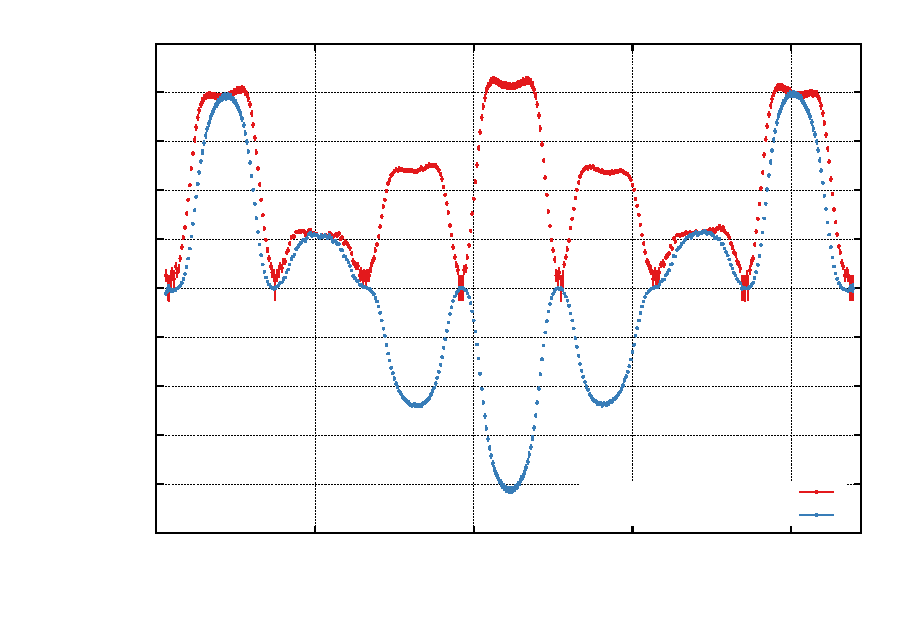
\includegraphics{./plots/PETRA-III/2_3_pi}}%
    \gplfronttext
  \end{picture}%
\endgroup

	\caption[Feldverteilung der $\mathrm{TM}_{010}\text{-}\frac{2}{3}\pi$-Mode von PETRA-III]{Verteilung des longitudinalen elektrischen Feldes der $\mathrm{TM}_{010}\text{-}\frac{2}{3}\pi$-Mode von PETRA-III bei einer Resonanzfrequenz von \mbox{$\nu_0 = \SI{501.14}{MHz}$} im Vakuum.}
	
	% GNUPLOT: LaTeX picture with Postscript
\begingroup
  \makeatletter
  \providecommand\color[2][]{%
    \GenericError{(gnuplot) \space\space\space\@spaces}{%
      Package color not loaded in conjunction with
      terminal option `colourtext'%
    }{See the gnuplot documentation for explanation.%
    }{Either use 'blacktext' in gnuplot or load the package
      color.sty in LaTeX.}%
    \renewcommand\color[2][]{}%
  }%
  \providecommand\includegraphics[2][]{%
    \GenericError{(gnuplot) \space\space\space\@spaces}{%
      Package graphicx or graphics not loaded%
    }{See the gnuplot documentation for explanation.%
    }{The gnuplot epslatex terminal needs graphicx.sty or graphics.sty.}%
    \renewcommand\includegraphics[2][]{}%
  }%
  \providecommand\rotatebox[2]{#2}%
  \@ifundefined{ifGPcolor}{%
    \newif\ifGPcolor
    \GPcolortrue
  }{}%
  \@ifundefined{ifGPblacktext}{%
    \newif\ifGPblacktext
    \GPblacktexttrue
  }{}%
  % define a \g@addto@macro without @ in the name:
  \let\gplgaddtomacro\g@addto@macro
  % define empty templates for all commands taking text:
  \gdef\gplbacktext{}%
  \gdef\gplfronttext{}%
  \makeatother
  \ifGPblacktext
    % no textcolor at all
    \def\colorrgb#1{}%
    \def\colorgray#1{}%
  \else
    % gray or color?
    \ifGPcolor
      \def\colorrgb#1{\color[rgb]{#1}}%
      \def\colorgray#1{\color[gray]{#1}}%
      \expandafter\def\csname LTw\endcsname{\color{white}}%
      \expandafter\def\csname LTb\endcsname{\color{black}}%
      \expandafter\def\csname LTa\endcsname{\color{black}}%
      \expandafter\def\csname LT0\endcsname{\color[rgb]{1,0,0}}%
      \expandafter\def\csname LT1\endcsname{\color[rgb]{0,1,0}}%
      \expandafter\def\csname LT2\endcsname{\color[rgb]{0,0,1}}%
      \expandafter\def\csname LT3\endcsname{\color[rgb]{1,0,1}}%
      \expandafter\def\csname LT4\endcsname{\color[rgb]{0,1,1}}%
      \expandafter\def\csname LT5\endcsname{\color[rgb]{1,1,0}}%
      \expandafter\def\csname LT6\endcsname{\color[rgb]{0,0,0}}%
      \expandafter\def\csname LT7\endcsname{\color[rgb]{1,0.3,0}}%
      \expandafter\def\csname LT8\endcsname{\color[rgb]{0.5,0.5,0.5}}%
    \else
      % gray
      \def\colorrgb#1{\color{black}}%
      \def\colorgray#1{\color[gray]{#1}}%
      \expandafter\def\csname LTw\endcsname{\color{white}}%
      \expandafter\def\csname LTb\endcsname{\color{black}}%
      \expandafter\def\csname LTa\endcsname{\color{black}}%
      \expandafter\def\csname LT0\endcsname{\color{black}}%
      \expandafter\def\csname LT1\endcsname{\color{black}}%
      \expandafter\def\csname LT2\endcsname{\color{black}}%
      \expandafter\def\csname LT3\endcsname{\color{black}}%
      \expandafter\def\csname LT4\endcsname{\color{black}}%
      \expandafter\def\csname LT5\endcsname{\color{black}}%
      \expandafter\def\csname LT6\endcsname{\color{black}}%
      \expandafter\def\csname LT7\endcsname{\color{black}}%
      \expandafter\def\csname LT8\endcsname{\color{black}}%
    \fi
  \fi
    \setlength{\unitlength}{0.0500bp}%
    \ifx\gptboxheight\undefined%
      \newlength{\gptboxheight}%
      \newlength{\gptboxwidth}%
      \newsavebox{\gptboxtext}%
    \fi%
    \setlength{\fboxrule}{0.5pt}%
    \setlength{\fboxsep}{1pt}%
\begin{picture}(8502.00,5668.00)%
    \gplgaddtomacro\gplbacktext{%
      \csname LTb\endcsname%
      \put(1210,704){\makebox(0,0)[r]{\strut{}-10000}}%
      \csname LTb\endcsname%
      \put(1210,1174){\makebox(0,0)[r]{\strut{}-8000}}%
      \csname LTb\endcsname%
      \put(1210,1644){\makebox(0,0)[r]{\strut{}-6000}}%
      \csname LTb\endcsname%
      \put(1210,2114){\makebox(0,0)[r]{\strut{}-4000}}%
      \csname LTb\endcsname%
      \put(1210,2584){\makebox(0,0)[r]{\strut{}-2000}}%
      \csname LTb\endcsname%
      \put(1210,3054){\makebox(0,0)[r]{\strut{}0}}%
      \csname LTb\endcsname%
      \put(1210,3523){\makebox(0,0)[r]{\strut{}2000}}%
      \csname LTb\endcsname%
      \put(1210,3993){\makebox(0,0)[r]{\strut{}4000}}%
      \csname LTb\endcsname%
      \put(1210,4463){\makebox(0,0)[r]{\strut{}6000}}%
      \csname LTb\endcsname%
      \put(1210,4933){\makebox(0,0)[r]{\strut{}8000}}%
      \csname LTb\endcsname%
      \put(1210,5403){\makebox(0,0)[r]{\strut{}10000}}%
      \csname LTb\endcsname%
      \put(1342,484){\makebox(0,0){\strut{}0}}%
      \csname LTb\endcsname%
      \put(2865,484){\makebox(0,0){\strut{}500}}%
      \csname LTb\endcsname%
      \put(4388,484){\makebox(0,0){\strut{}1000}}%
      \csname LTb\endcsname%
      \put(5912,484){\makebox(0,0){\strut{}1500}}%
      \csname LTb\endcsname%
      \put(7435,484){\makebox(0,0){\strut{}2000}}%
    }%
    \gplgaddtomacro\gplfronttext{%
      \csname LTb\endcsname%
      \put(176,3053){\rotatebox{-270}{\makebox(0,0){\strut{}$\frac{E_0(z)}{\sqrt{P_\mathrm{V}}}$ / \si{\volt\per\metre\per\watt\tothe{0.5}}}}}%
      \put(4723,154){\makebox(0,0){\strut{}$z$ / \si{mm}}}%
      \csname LTb\endcsname%
      \put(7382,5230){\makebox(0,0)[r]{\strut{}Amplitude}}%
      \csname LTb\endcsname%
      \put(7382,5010){\makebox(0,0)[r]{\strut{}effektives Feld}}%
    }%
    \gplbacktext
    \put(0,0){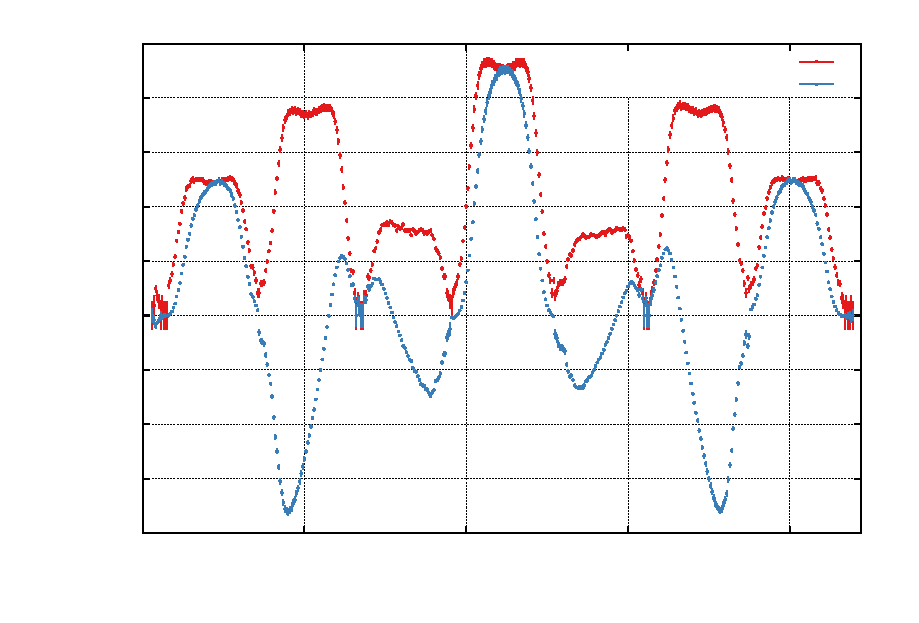
\includegraphics{./plots/PETRA-III/1_3_pi}}%
    \gplfronttext
  \end{picture}%
\endgroup

	\caption[Feldverteilung der $\mathrm{TM}_{010}\text{-}\frac{1}{3}\pi$-Mode von PETRA-III]{Verteilung des longitudinalen elektrischen Feldes der $\mathrm{TM}_{010}\text{-}\frac{1}{3}\pi$-Mode von PETRA-III bei einer Resonanzfrequenz von \mbox{$\nu_0 = \SI{505.37}{MHz}$} im Vakuum.}
\end{figure}

\begin{figure}[p]
  \centering
  % GNUPLOT: LaTeX picture with Postscript
\begingroup
  \makeatletter
  \providecommand\color[2][]{%
    \GenericError{(gnuplot) \space\space\space\@spaces}{%
      Package color not loaded in conjunction with
      terminal option `colourtext'%
    }{See the gnuplot documentation for explanation.%
    }{Either use 'blacktext' in gnuplot or load the package
      color.sty in LaTeX.}%
    \renewcommand\color[2][]{}%
  }%
  \providecommand\includegraphics[2][]{%
    \GenericError{(gnuplot) \space\space\space\@spaces}{%
      Package graphicx or graphics not loaded%
    }{See the gnuplot documentation for explanation.%
    }{The gnuplot epslatex terminal needs graphicx.sty or graphics.sty.}%
    \renewcommand\includegraphics[2][]{}%
  }%
  \providecommand\rotatebox[2]{#2}%
  \@ifundefined{ifGPcolor}{%
    \newif\ifGPcolor
    \GPcolortrue
  }{}%
  \@ifundefined{ifGPblacktext}{%
    \newif\ifGPblacktext
    \GPblacktexttrue
  }{}%
  % define a \g@addto@macro without @ in the name:
  \let\gplgaddtomacro\g@addto@macro
  % define empty templates for all commands taking text:
  \gdef\gplbacktext{}%
  \gdef\gplfronttext{}%
  \makeatother
  \ifGPblacktext
    % no textcolor at all
    \def\colorrgb#1{}%
    \def\colorgray#1{}%
  \else
    % gray or color?
    \ifGPcolor
      \def\colorrgb#1{\color[rgb]{#1}}%
      \def\colorgray#1{\color[gray]{#1}}%
      \expandafter\def\csname LTw\endcsname{\color{white}}%
      \expandafter\def\csname LTb\endcsname{\color{black}}%
      \expandafter\def\csname LTa\endcsname{\color{black}}%
      \expandafter\def\csname LT0\endcsname{\color[rgb]{1,0,0}}%
      \expandafter\def\csname LT1\endcsname{\color[rgb]{0,1,0}}%
      \expandafter\def\csname LT2\endcsname{\color[rgb]{0,0,1}}%
      \expandafter\def\csname LT3\endcsname{\color[rgb]{1,0,1}}%
      \expandafter\def\csname LT4\endcsname{\color[rgb]{0,1,1}}%
      \expandafter\def\csname LT5\endcsname{\color[rgb]{1,1,0}}%
      \expandafter\def\csname LT6\endcsname{\color[rgb]{0,0,0}}%
      \expandafter\def\csname LT7\endcsname{\color[rgb]{1,0.3,0}}%
      \expandafter\def\csname LT8\endcsname{\color[rgb]{0.5,0.5,0.5}}%
    \else
      % gray
      \def\colorrgb#1{\color{black}}%
      \def\colorgray#1{\color[gray]{#1}}%
      \expandafter\def\csname LTw\endcsname{\color{white}}%
      \expandafter\def\csname LTb\endcsname{\color{black}}%
      \expandafter\def\csname LTa\endcsname{\color{black}}%
      \expandafter\def\csname LT0\endcsname{\color{black}}%
      \expandafter\def\csname LT1\endcsname{\color{black}}%
      \expandafter\def\csname LT2\endcsname{\color{black}}%
      \expandafter\def\csname LT3\endcsname{\color{black}}%
      \expandafter\def\csname LT4\endcsname{\color{black}}%
      \expandafter\def\csname LT5\endcsname{\color{black}}%
      \expandafter\def\csname LT6\endcsname{\color{black}}%
      \expandafter\def\csname LT7\endcsname{\color{black}}%
      \expandafter\def\csname LT8\endcsname{\color{black}}%
    \fi
  \fi
    \setlength{\unitlength}{0.0500bp}%
    \ifx\gptboxheight\undefined%
      \newlength{\gptboxheight}%
      \newlength{\gptboxwidth}%
      \newsavebox{\gptboxtext}%
    \fi%
    \setlength{\fboxrule}{0.5pt}%
    \setlength{\fboxsep}{1pt}%
\begin{picture}(8502.00,5668.00)%
    \gplgaddtomacro\gplbacktext{%
      \csname LTb\endcsname%
      \put(1210,704){\makebox(0,0)[r]{\strut{}-10000}}%
      \csname LTb\endcsname%
      \put(1210,1174){\makebox(0,0)[r]{\strut{}-8000}}%
      \csname LTb\endcsname%
      \put(1210,1644){\makebox(0,0)[r]{\strut{}-6000}}%
      \csname LTb\endcsname%
      \put(1210,2114){\makebox(0,0)[r]{\strut{}-4000}}%
      \csname LTb\endcsname%
      \put(1210,2584){\makebox(0,0)[r]{\strut{}-2000}}%
      \csname LTb\endcsname%
      \put(1210,3054){\makebox(0,0)[r]{\strut{}0}}%
      \csname LTb\endcsname%
      \put(1210,3523){\makebox(0,0)[r]{\strut{}2000}}%
      \csname LTb\endcsname%
      \put(1210,3993){\makebox(0,0)[r]{\strut{}4000}}%
      \csname LTb\endcsname%
      \put(1210,4463){\makebox(0,0)[r]{\strut{}6000}}%
      \csname LTb\endcsname%
      \put(1210,4933){\makebox(0,0)[r]{\strut{}8000}}%
      \csname LTb\endcsname%
      \put(1210,5403){\makebox(0,0)[r]{\strut{}10000}}%
      \csname LTb\endcsname%
      \put(1342,484){\makebox(0,0){\strut{}0}}%
      \csname LTb\endcsname%
      \put(2865,484){\makebox(0,0){\strut{}500}}%
      \csname LTb\endcsname%
      \put(4388,484){\makebox(0,0){\strut{}1000}}%
      \csname LTb\endcsname%
      \put(5912,484){\makebox(0,0){\strut{}1500}}%
      \csname LTb\endcsname%
      \put(7435,484){\makebox(0,0){\strut{}2000}}%
    }%
    \gplgaddtomacro\gplfronttext{%
      \csname LTb\endcsname%
      \put(176,3053){\rotatebox{-270}{\makebox(0,0){\strut{}$\frac{E_0(z)}{\sqrt{P_\mathrm{V}}}$ / \si{\volt\per\metre\per\watt\tothe{0.5}}}}}%
      \put(4723,154){\makebox(0,0){\strut{}$z$ / \si{mm}}}%
      \csname LTb\endcsname%
      \put(7382,5230){\makebox(0,0)[r]{\strut{}Amplitude}}%
      \csname LTb\endcsname%
      \put(7382,5010){\makebox(0,0)[r]{\strut{}effektives Feld}}%
    }%
    \gplbacktext
    \put(0,0){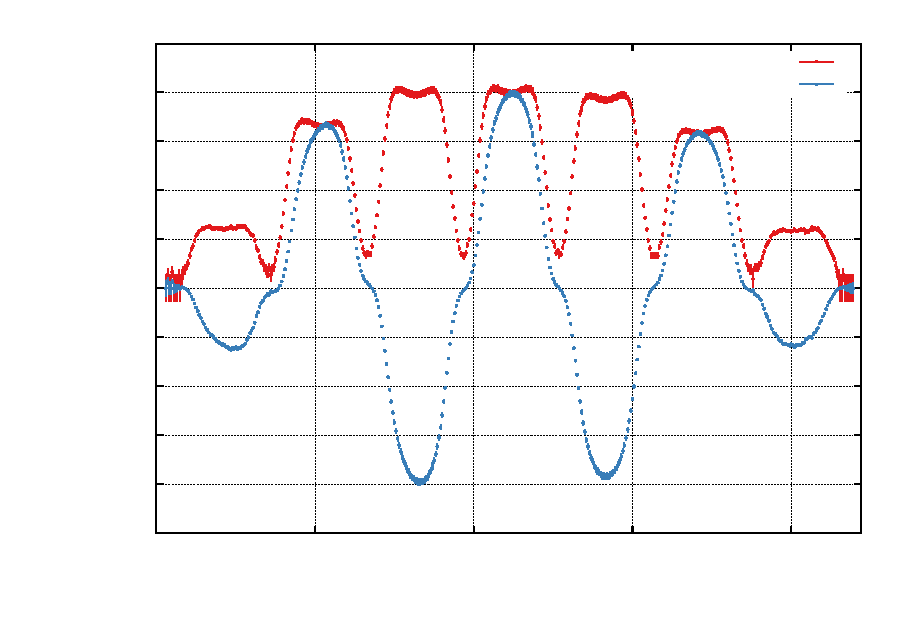
\includegraphics{./plots/PETRA-III/0_pi}}%
    \gplfronttext
  \end{picture}%
\endgroup

  \caption[Feldverteilung der $\mathrm{TM}_{010}\text{-}0$-Mode von PETRA-III]{Verteilung des longitudinalen elektrischen Feldes der $\mathrm{TM}_{010}\text{-}0$-Mode von PETRA-III bei einer Resonanzfrequenz von \mbox{$\nu_0 = \SI{508.61}{MHz}$} im Vakuum.}
\end{figure}
\FloatBarrier

\clearpage
\subsection{PETRA-IV}
\FloatBarrier

\vspace*{\fill}

\begin{figure}[h]
  \centering
  % GNUPLOT: LaTeX picture with Postscript
\begingroup
  \makeatletter
  \providecommand\color[2][]{%
    \GenericError{(gnuplot) \space\space\space\@spaces}{%
      Package color not loaded in conjunction with
      terminal option `colourtext'%
    }{See the gnuplot documentation for explanation.%
    }{Either use 'blacktext' in gnuplot or load the package
      color.sty in LaTeX.}%
    \renewcommand\color[2][]{}%
  }%
  \providecommand\includegraphics[2][]{%
    \GenericError{(gnuplot) \space\space\space\@spaces}{%
      Package graphicx or graphics not loaded%
    }{See the gnuplot documentation for explanation.%
    }{The gnuplot epslatex terminal needs graphicx.sty or graphics.sty.}%
    \renewcommand\includegraphics[2][]{}%
  }%
  \providecommand\rotatebox[2]{#2}%
  \@ifundefined{ifGPcolor}{%
    \newif\ifGPcolor
    \GPcolortrue
  }{}%
  \@ifundefined{ifGPblacktext}{%
    \newif\ifGPblacktext
    \GPblacktexttrue
  }{}%
  % define a \g@addto@macro without @ in the name:
  \let\gplgaddtomacro\g@addto@macro
  % define empty templates for all commands taking text:
  \gdef\gplbacktext{}%
  \gdef\gplfronttext{}%
  \makeatother
  \ifGPblacktext
    % no textcolor at all
    \def\colorrgb#1{}%
    \def\colorgray#1{}%
  \else
    % gray or color?
    \ifGPcolor
      \def\colorrgb#1{\color[rgb]{#1}}%
      \def\colorgray#1{\color[gray]{#1}}%
      \expandafter\def\csname LTw\endcsname{\color{white}}%
      \expandafter\def\csname LTb\endcsname{\color{black}}%
      \expandafter\def\csname LTa\endcsname{\color{black}}%
      \expandafter\def\csname LT0\endcsname{\color[rgb]{1,0,0}}%
      \expandafter\def\csname LT1\endcsname{\color[rgb]{0,1,0}}%
      \expandafter\def\csname LT2\endcsname{\color[rgb]{0,0,1}}%
      \expandafter\def\csname LT3\endcsname{\color[rgb]{1,0,1}}%
      \expandafter\def\csname LT4\endcsname{\color[rgb]{0,1,1}}%
      \expandafter\def\csname LT5\endcsname{\color[rgb]{1,1,0}}%
      \expandafter\def\csname LT6\endcsname{\color[rgb]{0,0,0}}%
      \expandafter\def\csname LT7\endcsname{\color[rgb]{1,0.3,0}}%
      \expandafter\def\csname LT8\endcsname{\color[rgb]{0.5,0.5,0.5}}%
    \else
      % gray
      \def\colorrgb#1{\color{black}}%
      \def\colorgray#1{\color[gray]{#1}}%
      \expandafter\def\csname LTw\endcsname{\color{white}}%
      \expandafter\def\csname LTb\endcsname{\color{black}}%
      \expandafter\def\csname LTa\endcsname{\color{black}}%
      \expandafter\def\csname LT0\endcsname{\color{black}}%
      \expandafter\def\csname LT1\endcsname{\color{black}}%
      \expandafter\def\csname LT2\endcsname{\color{black}}%
      \expandafter\def\csname LT3\endcsname{\color{black}}%
      \expandafter\def\csname LT4\endcsname{\color{black}}%
      \expandafter\def\csname LT5\endcsname{\color{black}}%
      \expandafter\def\csname LT6\endcsname{\color{black}}%
      \expandafter\def\csname LT7\endcsname{\color{black}}%
      \expandafter\def\csname LT8\endcsname{\color{black}}%
    \fi
  \fi
    \setlength{\unitlength}{0.0500bp}%
    \ifx\gptboxheight\undefined%
      \newlength{\gptboxheight}%
      \newlength{\gptboxwidth}%
      \newsavebox{\gptboxtext}%
    \fi%
    \setlength{\fboxrule}{0.5pt}%
    \setlength{\fboxsep}{1pt}%
\begin{picture}(8502.00,5668.00)%
    \gplgaddtomacro\gplbacktext{%
      \csname LTb\endcsname%
      \put(1078,704){\makebox(0,0)[r]{\strut{}-1000}}%
      \csname LTb\endcsname%
      \put(1078,1291){\makebox(0,0)[r]{\strut{}0}}%
      \csname LTb\endcsname%
      \put(1078,1879){\makebox(0,0)[r]{\strut{}1000}}%
      \csname LTb\endcsname%
      \put(1078,2466){\makebox(0,0)[r]{\strut{}2000}}%
      \csname LTb\endcsname%
      \put(1078,3054){\makebox(0,0)[r]{\strut{}3000}}%
      \csname LTb\endcsname%
      \put(1078,3641){\makebox(0,0)[r]{\strut{}4000}}%
      \csname LTb\endcsname%
      \put(1078,4228){\makebox(0,0)[r]{\strut{}5000}}%
      \csname LTb\endcsname%
      \put(1078,4816){\makebox(0,0)[r]{\strut{}6000}}%
      \csname LTb\endcsname%
      \put(1078,5403){\makebox(0,0)[r]{\strut{}7000}}%
      \csname LTb\endcsname%
      \put(1210,484){\makebox(0,0){\strut{}0}}%
      \csname LTb\endcsname%
      \put(2763,484){\makebox(0,0){\strut{}500}}%
      \csname LTb\endcsname%
      \put(4316,484){\makebox(0,0){\strut{}1000}}%
      \csname LTb\endcsname%
      \put(5869,484){\makebox(0,0){\strut{}1500}}%
      \csname LTb\endcsname%
      \put(7422,484){\makebox(0,0){\strut{}2000}}%
    }%
    \gplgaddtomacro\gplfronttext{%
      \csname LTb\endcsname%
      \put(176,3053){\rotatebox{-270}{\makebox(0,0){\strut{}$\frac{E_0(z)}{\sqrt{P_\mathrm{V}}}$ / \si{\volt\per\metre\per\watt\tothe{0{,}5}}}}}%
      \put(4657,154){\makebox(0,0){\strut{}$z$ / \si{mm}}}%
      \csname LTb\endcsname%
      \put(7382,5230){\makebox(0,0)[r]{\strut{}Amplitude}}%
      \csname LTb\endcsname%
      \put(7382,5010){\makebox(0,0)[r]{\strut{}effektives Feld}}%
    }%
    \gplbacktext
    \put(0,0){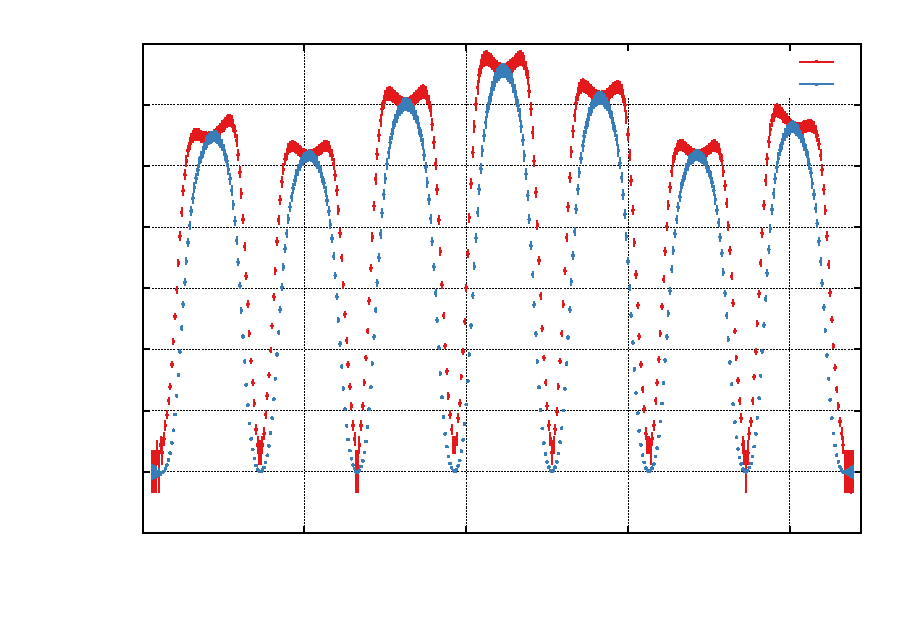
\includegraphics{./plots/PETRA-IV/pi}}%
    \gplfronttext
  \end{picture}%
\endgroup

  \caption[Feldverteilung der $\mathrm{TM}_{010}\text{-}\pi$-Mode von PETRA-IV]{Verteilung des longitudinalen elektrischen Feldes der $\mathrm{TM}_{010}\text{-}\pi$-Mode von PETRA-IV bei einer Resonanzfrequenz von \mbox{$\nu_0 = \SI{499.67}{MHz}$} im Vakuum.}
\end{figure}

\vspace*{\fill}

\begin{figure}[p]
	\centering
  
	% GNUPLOT: LaTeX picture with Postscript
\begingroup
  \makeatletter
  \providecommand\color[2][]{%
    \GenericError{(gnuplot) \space\space\space\@spaces}{%
      Package color not loaded in conjunction with
      terminal option `colourtext'%
    }{See the gnuplot documentation for explanation.%
    }{Either use 'blacktext' in gnuplot or load the package
      color.sty in LaTeX.}%
    \renewcommand\color[2][]{}%
  }%
  \providecommand\includegraphics[2][]{%
    \GenericError{(gnuplot) \space\space\space\@spaces}{%
      Package graphicx or graphics not loaded%
    }{See the gnuplot documentation for explanation.%
    }{The gnuplot epslatex terminal needs graphicx.sty or graphics.sty.}%
    \renewcommand\includegraphics[2][]{}%
  }%
  \providecommand\rotatebox[2]{#2}%
  \@ifundefined{ifGPcolor}{%
    \newif\ifGPcolor
    \GPcolortrue
  }{}%
  \@ifundefined{ifGPblacktext}{%
    \newif\ifGPblacktext
    \GPblacktexttrue
  }{}%
  % define a \g@addto@macro without @ in the name:
  \let\gplgaddtomacro\g@addto@macro
  % define empty templates for all commands taking text:
  \gdef\gplbacktext{}%
  \gdef\gplfronttext{}%
  \makeatother
  \ifGPblacktext
    % no textcolor at all
    \def\colorrgb#1{}%
    \def\colorgray#1{}%
  \else
    % gray or color?
    \ifGPcolor
      \def\colorrgb#1{\color[rgb]{#1}}%
      \def\colorgray#1{\color[gray]{#1}}%
      \expandafter\def\csname LTw\endcsname{\color{white}}%
      \expandafter\def\csname LTb\endcsname{\color{black}}%
      \expandafter\def\csname LTa\endcsname{\color{black}}%
      \expandafter\def\csname LT0\endcsname{\color[rgb]{1,0,0}}%
      \expandafter\def\csname LT1\endcsname{\color[rgb]{0,1,0}}%
      \expandafter\def\csname LT2\endcsname{\color[rgb]{0,0,1}}%
      \expandafter\def\csname LT3\endcsname{\color[rgb]{1,0,1}}%
      \expandafter\def\csname LT4\endcsname{\color[rgb]{0,1,1}}%
      \expandafter\def\csname LT5\endcsname{\color[rgb]{1,1,0}}%
      \expandafter\def\csname LT6\endcsname{\color[rgb]{0,0,0}}%
      \expandafter\def\csname LT7\endcsname{\color[rgb]{1,0.3,0}}%
      \expandafter\def\csname LT8\endcsname{\color[rgb]{0.5,0.5,0.5}}%
    \else
      % gray
      \def\colorrgb#1{\color{black}}%
      \def\colorgray#1{\color[gray]{#1}}%
      \expandafter\def\csname LTw\endcsname{\color{white}}%
      \expandafter\def\csname LTb\endcsname{\color{black}}%
      \expandafter\def\csname LTa\endcsname{\color{black}}%
      \expandafter\def\csname LT0\endcsname{\color{black}}%
      \expandafter\def\csname LT1\endcsname{\color{black}}%
      \expandafter\def\csname LT2\endcsname{\color{black}}%
      \expandafter\def\csname LT3\endcsname{\color{black}}%
      \expandafter\def\csname LT4\endcsname{\color{black}}%
      \expandafter\def\csname LT5\endcsname{\color{black}}%
      \expandafter\def\csname LT6\endcsname{\color{black}}%
      \expandafter\def\csname LT7\endcsname{\color{black}}%
      \expandafter\def\csname LT8\endcsname{\color{black}}%
    \fi
  \fi
    \setlength{\unitlength}{0.0500bp}%
    \ifx\gptboxheight\undefined%
      \newlength{\gptboxheight}%
      \newlength{\gptboxwidth}%
      \newsavebox{\gptboxtext}%
    \fi%
    \setlength{\fboxrule}{0.5pt}%
    \setlength{\fboxsep}{1pt}%
\begin{picture}(8502.00,5668.00)%
    \gplgaddtomacro\gplbacktext{%
      \csname LTb\endcsname%
      \put(1210,704){\makebox(0,0)[r]{\strut{}-10000}}%
      \csname LTb\endcsname%
      \put(1210,1174){\makebox(0,0)[r]{\strut{}-8000}}%
      \csname LTb\endcsname%
      \put(1210,1644){\makebox(0,0)[r]{\strut{}-6000}}%
      \csname LTb\endcsname%
      \put(1210,2114){\makebox(0,0)[r]{\strut{}-4000}}%
      \csname LTb\endcsname%
      \put(1210,2584){\makebox(0,0)[r]{\strut{}-2000}}%
      \csname LTb\endcsname%
      \put(1210,3054){\makebox(0,0)[r]{\strut{}0}}%
      \csname LTb\endcsname%
      \put(1210,3523){\makebox(0,0)[r]{\strut{}2000}}%
      \csname LTb\endcsname%
      \put(1210,3993){\makebox(0,0)[r]{\strut{}4000}}%
      \csname LTb\endcsname%
      \put(1210,4463){\makebox(0,0)[r]{\strut{}6000}}%
      \csname LTb\endcsname%
      \put(1210,4933){\makebox(0,0)[r]{\strut{}8000}}%
      \csname LTb\endcsname%
      \put(1210,5403){\makebox(0,0)[r]{\strut{}10000}}%
      \csname LTb\endcsname%
      \put(1342,484){\makebox(0,0){\strut{}0}}%
      \csname LTb\endcsname%
      \put(2865,484){\makebox(0,0){\strut{}500}}%
      \csname LTb\endcsname%
      \put(4388,484){\makebox(0,0){\strut{}1000}}%
      \csname LTb\endcsname%
      \put(5912,484){\makebox(0,0){\strut{}1500}}%
      \csname LTb\endcsname%
      \put(7435,484){\makebox(0,0){\strut{}2000}}%
    }%
    \gplgaddtomacro\gplfronttext{%
      \csname LTb\endcsname%
      \put(176,3053){\rotatebox{-270}{\makebox(0,0){\strut{}$\frac{E_0(z)}{\sqrt{P_\mathrm{V}}}$ / \si{\volt\per\metre\per\watt\tothe{0.5}}}}}%
      \put(4723,154){\makebox(0,0){\strut{}$z$ / \si{mm}}}%
      \csname LTb\endcsname%
      \put(7382,5230){\makebox(0,0)[r]{\strut{}Amplitude}}%
      \csname LTb\endcsname%
      \put(7382,5010){\makebox(0,0)[r]{\strut{}effektives Feld}}%
    }%
    \gplbacktext
    \put(0,0){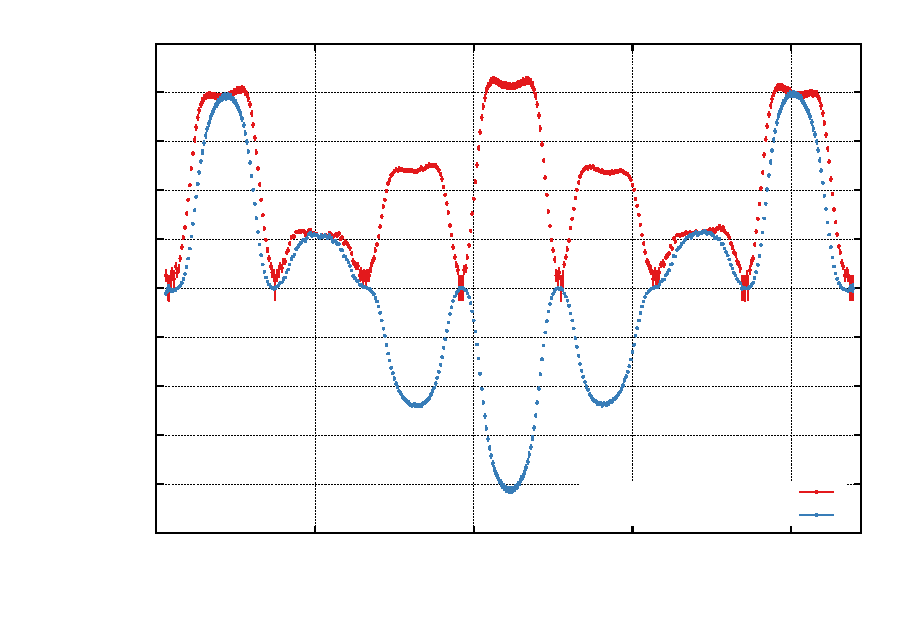
\includegraphics{./plots/PETRA-III/2_3_pi}}%
    \gplfronttext
  \end{picture}%
\endgroup

	\caption[Feldverteilung der $\mathrm{TM}_{010}\text{-}\frac{2}{3}\pi$-Mode von PETRA-IV]{Verteilung des longitudinalen elektrischen Feldes der $\mathrm{TM}_{010}\text{-}\frac{2}{3}\pi$-Mode von PETRA-IV bei einer Resonanzfrequenz von \mbox{$\nu_0 = \SI{501.17}{MHz}$} im Vakuum.}
	
    % GNUPLOT: LaTeX picture with Postscript
\begingroup
  \makeatletter
  \providecommand\color[2][]{%
    \GenericError{(gnuplot) \space\space\space\@spaces}{%
      Package color not loaded in conjunction with
      terminal option `colourtext'%
    }{See the gnuplot documentation for explanation.%
    }{Either use 'blacktext' in gnuplot or load the package
      color.sty in LaTeX.}%
    \renewcommand\color[2][]{}%
  }%
  \providecommand\includegraphics[2][]{%
    \GenericError{(gnuplot) \space\space\space\@spaces}{%
      Package graphicx or graphics not loaded%
    }{See the gnuplot documentation for explanation.%
    }{The gnuplot epslatex terminal needs graphicx.sty or graphics.sty.}%
    \renewcommand\includegraphics[2][]{}%
  }%
  \providecommand\rotatebox[2]{#2}%
  \@ifundefined{ifGPcolor}{%
    \newif\ifGPcolor
    \GPcolortrue
  }{}%
  \@ifundefined{ifGPblacktext}{%
    \newif\ifGPblacktext
    \GPblacktexttrue
  }{}%
  % define a \g@addto@macro without @ in the name:
  \let\gplgaddtomacro\g@addto@macro
  % define empty templates for all commands taking text:
  \gdef\gplbacktext{}%
  \gdef\gplfronttext{}%
  \makeatother
  \ifGPblacktext
    % no textcolor at all
    \def\colorrgb#1{}%
    \def\colorgray#1{}%
  \else
    % gray or color?
    \ifGPcolor
      \def\colorrgb#1{\color[rgb]{#1}}%
      \def\colorgray#1{\color[gray]{#1}}%
      \expandafter\def\csname LTw\endcsname{\color{white}}%
      \expandafter\def\csname LTb\endcsname{\color{black}}%
      \expandafter\def\csname LTa\endcsname{\color{black}}%
      \expandafter\def\csname LT0\endcsname{\color[rgb]{1,0,0}}%
      \expandafter\def\csname LT1\endcsname{\color[rgb]{0,1,0}}%
      \expandafter\def\csname LT2\endcsname{\color[rgb]{0,0,1}}%
      \expandafter\def\csname LT3\endcsname{\color[rgb]{1,0,1}}%
      \expandafter\def\csname LT4\endcsname{\color[rgb]{0,1,1}}%
      \expandafter\def\csname LT5\endcsname{\color[rgb]{1,1,0}}%
      \expandafter\def\csname LT6\endcsname{\color[rgb]{0,0,0}}%
      \expandafter\def\csname LT7\endcsname{\color[rgb]{1,0.3,0}}%
      \expandafter\def\csname LT8\endcsname{\color[rgb]{0.5,0.5,0.5}}%
    \else
      % gray
      \def\colorrgb#1{\color{black}}%
      \def\colorgray#1{\color[gray]{#1}}%
      \expandafter\def\csname LTw\endcsname{\color{white}}%
      \expandafter\def\csname LTb\endcsname{\color{black}}%
      \expandafter\def\csname LTa\endcsname{\color{black}}%
      \expandafter\def\csname LT0\endcsname{\color{black}}%
      \expandafter\def\csname LT1\endcsname{\color{black}}%
      \expandafter\def\csname LT2\endcsname{\color{black}}%
      \expandafter\def\csname LT3\endcsname{\color{black}}%
      \expandafter\def\csname LT4\endcsname{\color{black}}%
      \expandafter\def\csname LT5\endcsname{\color{black}}%
      \expandafter\def\csname LT6\endcsname{\color{black}}%
      \expandafter\def\csname LT7\endcsname{\color{black}}%
      \expandafter\def\csname LT8\endcsname{\color{black}}%
    \fi
  \fi
    \setlength{\unitlength}{0.0500bp}%
    \ifx\gptboxheight\undefined%
      \newlength{\gptboxheight}%
      \newlength{\gptboxwidth}%
      \newsavebox{\gptboxtext}%
    \fi%
    \setlength{\fboxrule}{0.5pt}%
    \setlength{\fboxsep}{1pt}%
\begin{picture}(8502.00,5668.00)%
    \gplgaddtomacro\gplbacktext{%
      \csname LTb\endcsname%
      \put(1210,704){\makebox(0,0)[r]{\strut{}-10000}}%
      \csname LTb\endcsname%
      \put(1210,1174){\makebox(0,0)[r]{\strut{}-8000}}%
      \csname LTb\endcsname%
      \put(1210,1644){\makebox(0,0)[r]{\strut{}-6000}}%
      \csname LTb\endcsname%
      \put(1210,2114){\makebox(0,0)[r]{\strut{}-4000}}%
      \csname LTb\endcsname%
      \put(1210,2584){\makebox(0,0)[r]{\strut{}-2000}}%
      \csname LTb\endcsname%
      \put(1210,3054){\makebox(0,0)[r]{\strut{}0}}%
      \csname LTb\endcsname%
      \put(1210,3523){\makebox(0,0)[r]{\strut{}2000}}%
      \csname LTb\endcsname%
      \put(1210,3993){\makebox(0,0)[r]{\strut{}4000}}%
      \csname LTb\endcsname%
      \put(1210,4463){\makebox(0,0)[r]{\strut{}6000}}%
      \csname LTb\endcsname%
      \put(1210,4933){\makebox(0,0)[r]{\strut{}8000}}%
      \csname LTb\endcsname%
      \put(1210,5403){\makebox(0,0)[r]{\strut{}10000}}%
      \csname LTb\endcsname%
      \put(1342,484){\makebox(0,0){\strut{}0}}%
      \csname LTb\endcsname%
      \put(2865,484){\makebox(0,0){\strut{}500}}%
      \csname LTb\endcsname%
      \put(4388,484){\makebox(0,0){\strut{}1000}}%
      \csname LTb\endcsname%
      \put(5912,484){\makebox(0,0){\strut{}1500}}%
      \csname LTb\endcsname%
      \put(7435,484){\makebox(0,0){\strut{}2000}}%
    }%
    \gplgaddtomacro\gplfronttext{%
      \csname LTb\endcsname%
      \put(176,3053){\rotatebox{-270}{\makebox(0,0){\strut{}$\frac{E_0(z)}{\sqrt{P_\mathrm{V}}}$ / \si{\volt\per\metre\per\watt\tothe{0.5}}}}}%
      \put(4723,154){\makebox(0,0){\strut{}$z$ / \si{mm}}}%
      \csname LTb\endcsname%
      \put(7382,5230){\makebox(0,0)[r]{\strut{}Amplitude}}%
      \csname LTb\endcsname%
      \put(7382,5010){\makebox(0,0)[r]{\strut{}effektives Feld}}%
    }%
    \gplbacktext
    \put(0,0){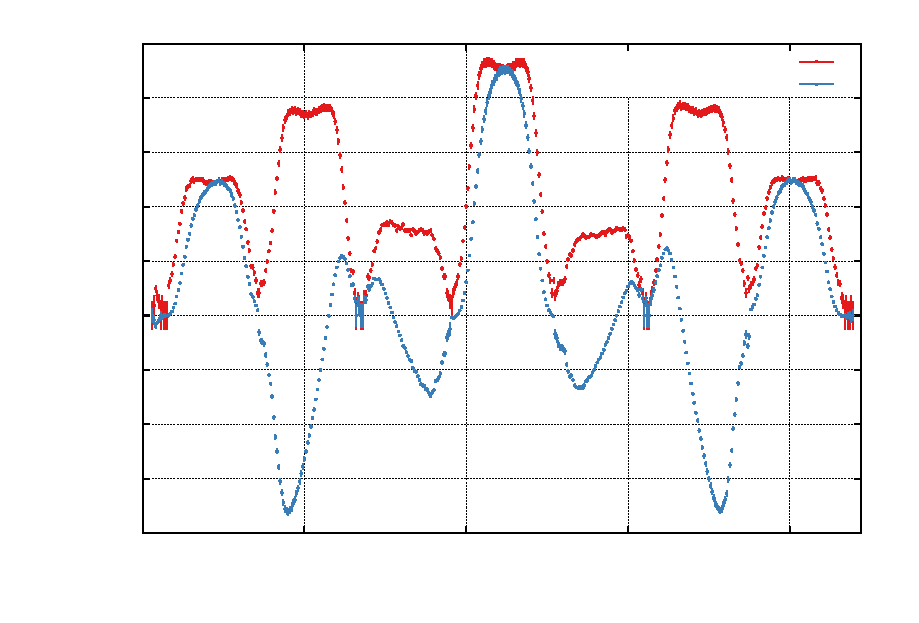
\includegraphics{./plots/PETRA-III/1_3_pi}}%
    \gplfronttext
  \end{picture}%
\endgroup

    \caption[Feldverteilung der $\mathrm{TM}_{010}\text{-}\frac{1}{3}\pi$-Mode von PETRA-IV]{Verteilung des longitudinalen elektrischen Feldes der $\mathrm{TM}_{010}\text{-}\frac{1}{3}\pi$-Mode von PETRA-IV bei einer Resonanzfrequenz von \mbox{$\nu_0 = \SI{505.43}{MHz}$} im Vakuum.}
\end{figure}

\begin{figure}[h]
  \centering
  % GNUPLOT: LaTeX picture with Postscript
\begingroup
  \makeatletter
  \providecommand\color[2][]{%
    \GenericError{(gnuplot) \space\space\space\@spaces}{%
      Package color not loaded in conjunction with
      terminal option `colourtext'%
    }{See the gnuplot documentation for explanation.%
    }{Either use 'blacktext' in gnuplot or load the package
      color.sty in LaTeX.}%
    \renewcommand\color[2][]{}%
  }%
  \providecommand\includegraphics[2][]{%
    \GenericError{(gnuplot) \space\space\space\@spaces}{%
      Package graphicx or graphics not loaded%
    }{See the gnuplot documentation for explanation.%
    }{The gnuplot epslatex terminal needs graphicx.sty or graphics.sty.}%
    \renewcommand\includegraphics[2][]{}%
  }%
  \providecommand\rotatebox[2]{#2}%
  \@ifundefined{ifGPcolor}{%
    \newif\ifGPcolor
    \GPcolortrue
  }{}%
  \@ifundefined{ifGPblacktext}{%
    \newif\ifGPblacktext
    \GPblacktexttrue
  }{}%
  % define a \g@addto@macro without @ in the name:
  \let\gplgaddtomacro\g@addto@macro
  % define empty templates for all commands taking text:
  \gdef\gplbacktext{}%
  \gdef\gplfronttext{}%
  \makeatother
  \ifGPblacktext
    % no textcolor at all
    \def\colorrgb#1{}%
    \def\colorgray#1{}%
  \else
    % gray or color?
    \ifGPcolor
      \def\colorrgb#1{\color[rgb]{#1}}%
      \def\colorgray#1{\color[gray]{#1}}%
      \expandafter\def\csname LTw\endcsname{\color{white}}%
      \expandafter\def\csname LTb\endcsname{\color{black}}%
      \expandafter\def\csname LTa\endcsname{\color{black}}%
      \expandafter\def\csname LT0\endcsname{\color[rgb]{1,0,0}}%
      \expandafter\def\csname LT1\endcsname{\color[rgb]{0,1,0}}%
      \expandafter\def\csname LT2\endcsname{\color[rgb]{0,0,1}}%
      \expandafter\def\csname LT3\endcsname{\color[rgb]{1,0,1}}%
      \expandafter\def\csname LT4\endcsname{\color[rgb]{0,1,1}}%
      \expandafter\def\csname LT5\endcsname{\color[rgb]{1,1,0}}%
      \expandafter\def\csname LT6\endcsname{\color[rgb]{0,0,0}}%
      \expandafter\def\csname LT7\endcsname{\color[rgb]{1,0.3,0}}%
      \expandafter\def\csname LT8\endcsname{\color[rgb]{0.5,0.5,0.5}}%
    \else
      % gray
      \def\colorrgb#1{\color{black}}%
      \def\colorgray#1{\color[gray]{#1}}%
      \expandafter\def\csname LTw\endcsname{\color{white}}%
      \expandafter\def\csname LTb\endcsname{\color{black}}%
      \expandafter\def\csname LTa\endcsname{\color{black}}%
      \expandafter\def\csname LT0\endcsname{\color{black}}%
      \expandafter\def\csname LT1\endcsname{\color{black}}%
      \expandafter\def\csname LT2\endcsname{\color{black}}%
      \expandafter\def\csname LT3\endcsname{\color{black}}%
      \expandafter\def\csname LT4\endcsname{\color{black}}%
      \expandafter\def\csname LT5\endcsname{\color{black}}%
      \expandafter\def\csname LT6\endcsname{\color{black}}%
      \expandafter\def\csname LT7\endcsname{\color{black}}%
      \expandafter\def\csname LT8\endcsname{\color{black}}%
    \fi
  \fi
    \setlength{\unitlength}{0.0500bp}%
    \ifx\gptboxheight\undefined%
      \newlength{\gptboxheight}%
      \newlength{\gptboxwidth}%
      \newsavebox{\gptboxtext}%
    \fi%
    \setlength{\fboxrule}{0.5pt}%
    \setlength{\fboxsep}{1pt}%
\begin{picture}(8502.00,5668.00)%
    \gplgaddtomacro\gplbacktext{%
      \csname LTb\endcsname%
      \put(1210,704){\makebox(0,0)[r]{\strut{}-10000}}%
      \csname LTb\endcsname%
      \put(1210,1174){\makebox(0,0)[r]{\strut{}-8000}}%
      \csname LTb\endcsname%
      \put(1210,1644){\makebox(0,0)[r]{\strut{}-6000}}%
      \csname LTb\endcsname%
      \put(1210,2114){\makebox(0,0)[r]{\strut{}-4000}}%
      \csname LTb\endcsname%
      \put(1210,2584){\makebox(0,0)[r]{\strut{}-2000}}%
      \csname LTb\endcsname%
      \put(1210,3054){\makebox(0,0)[r]{\strut{}0}}%
      \csname LTb\endcsname%
      \put(1210,3523){\makebox(0,0)[r]{\strut{}2000}}%
      \csname LTb\endcsname%
      \put(1210,3993){\makebox(0,0)[r]{\strut{}4000}}%
      \csname LTb\endcsname%
      \put(1210,4463){\makebox(0,0)[r]{\strut{}6000}}%
      \csname LTb\endcsname%
      \put(1210,4933){\makebox(0,0)[r]{\strut{}8000}}%
      \csname LTb\endcsname%
      \put(1210,5403){\makebox(0,0)[r]{\strut{}10000}}%
      \csname LTb\endcsname%
      \put(1342,484){\makebox(0,0){\strut{}0}}%
      \csname LTb\endcsname%
      \put(2865,484){\makebox(0,0){\strut{}500}}%
      \csname LTb\endcsname%
      \put(4388,484){\makebox(0,0){\strut{}1000}}%
      \csname LTb\endcsname%
      \put(5912,484){\makebox(0,0){\strut{}1500}}%
      \csname LTb\endcsname%
      \put(7435,484){\makebox(0,0){\strut{}2000}}%
    }%
    \gplgaddtomacro\gplfronttext{%
      \csname LTb\endcsname%
      \put(176,3053){\rotatebox{-270}{\makebox(0,0){\strut{}$\frac{E_0(z)}{\sqrt{P_\mathrm{V}}}$ / \si{\volt\per\metre\per\watt\tothe{0.5}}}}}%
      \put(4723,154){\makebox(0,0){\strut{}$z$ / \si{mm}}}%
      \csname LTb\endcsname%
      \put(7382,5230){\makebox(0,0)[r]{\strut{}Amplitude}}%
      \csname LTb\endcsname%
      \put(7382,5010){\makebox(0,0)[r]{\strut{}effektives Feld}}%
    }%
    \gplbacktext
    \put(0,0){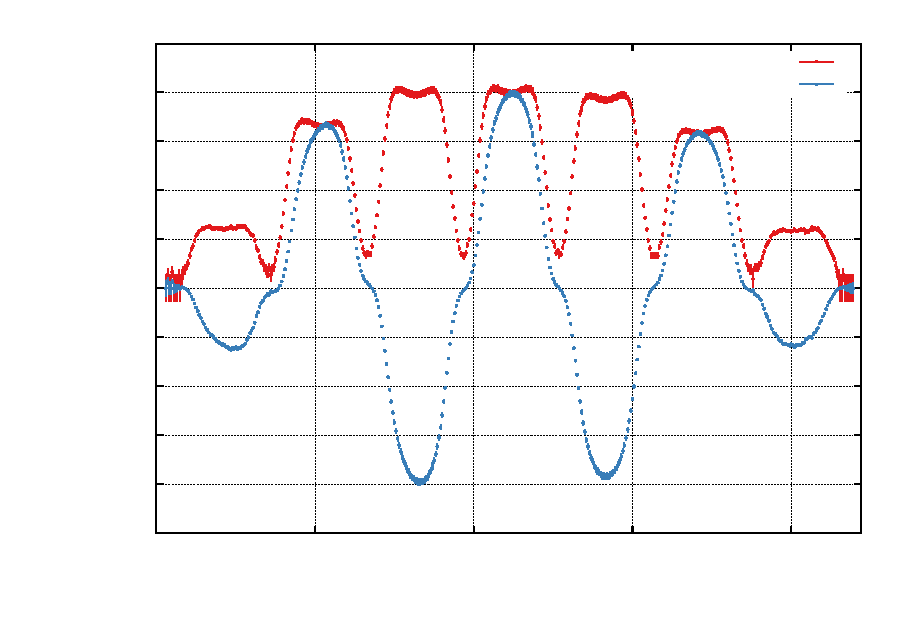
\includegraphics{./plots/PETRA-III/0_pi}}%
    \gplfronttext
  \end{picture}%
\endgroup

  \caption[Feldverteilung der $\mathrm{TM}_{010}\text{-}0$-Mode von PETRA-IV]{Verteilung des longitudinalen elektrischen Feldes der $\mathrm{TM}_{010}\text{-}0$-Mode von PETRA-IV bei einer Resonanzfrequenz von \mbox{$\nu_0 = \SI{508.61}{MHz}$} im Vakuum.}
\end{figure}
\FloatBarrier

\clearpage
%------------------------------------------------------------------------------
\section{Elektrische Feldverteilung von Resonatormoden höherer Ordnung}
\label{app:hom_felder}
%------------------------------------------------------------------------------
\FloatBarrier
Im Folgenden werden die Feldverteilungen der vermessenen Moden höherer Ordnung des Resonators PETRA-III zusammengetragen.
In allen Fällen ist die Position~$z$ relativ zum Vakuumflansch des Resonators und die elektrischen Felder normiert auf die Wurzel der Verlustleistung~$P_\mathrm{V}$ angegeben.
\begin{figure}[h]
  \centering
  % GNUPLOT: LaTeX picture with Postscript
\begingroup
  \makeatletter
  \providecommand\color[2][]{%
    \GenericError{(gnuplot) \space\space\space\@spaces}{%
      Package color not loaded in conjunction with
      terminal option `colourtext'%
    }{See the gnuplot documentation for explanation.%
    }{Either use 'blacktext' in gnuplot or load the package
      color.sty in LaTeX.}%
    \renewcommand\color[2][]{}%
  }%
  \providecommand\includegraphics[2][]{%
    \GenericError{(gnuplot) \space\space\space\@spaces}{%
      Package graphicx or graphics not loaded%
    }{See the gnuplot documentation for explanation.%
    }{The gnuplot epslatex terminal needs graphicx.sty or graphics.sty.}%
    \renewcommand\includegraphics[2][]{}%
  }%
  \providecommand\rotatebox[2]{#2}%
  \@ifundefined{ifGPcolor}{%
    \newif\ifGPcolor
    \GPcolortrue
  }{}%
  \@ifundefined{ifGPblacktext}{%
    \newif\ifGPblacktext
    \GPblacktexttrue
  }{}%
  % define a \g@addto@macro without @ in the name:
  \let\gplgaddtomacro\g@addto@macro
  % define empty templates for all commands taking text:
  \gdef\gplbacktext{}%
  \gdef\gplfronttext{}%
  \makeatother
  \ifGPblacktext
    % no textcolor at all
    \def\colorrgb#1{}%
    \def\colorgray#1{}%
  \else
    % gray or color?
    \ifGPcolor
      \def\colorrgb#1{\color[rgb]{#1}}%
      \def\colorgray#1{\color[gray]{#1}}%
      \expandafter\def\csname LTw\endcsname{\color{white}}%
      \expandafter\def\csname LTb\endcsname{\color{black}}%
      \expandafter\def\csname LTa\endcsname{\color{black}}%
      \expandafter\def\csname LT0\endcsname{\color[rgb]{1,0,0}}%
      \expandafter\def\csname LT1\endcsname{\color[rgb]{0,1,0}}%
      \expandafter\def\csname LT2\endcsname{\color[rgb]{0,0,1}}%
      \expandafter\def\csname LT3\endcsname{\color[rgb]{1,0,1}}%
      \expandafter\def\csname LT4\endcsname{\color[rgb]{0,1,1}}%
      \expandafter\def\csname LT5\endcsname{\color[rgb]{1,1,0}}%
      \expandafter\def\csname LT6\endcsname{\color[rgb]{0,0,0}}%
      \expandafter\def\csname LT7\endcsname{\color[rgb]{1,0.3,0}}%
      \expandafter\def\csname LT8\endcsname{\color[rgb]{0.5,0.5,0.5}}%
    \else
      % gray
      \def\colorrgb#1{\color{black}}%
      \def\colorgray#1{\color[gray]{#1}}%
      \expandafter\def\csname LTw\endcsname{\color{white}}%
      \expandafter\def\csname LTb\endcsname{\color{black}}%
      \expandafter\def\csname LTa\endcsname{\color{black}}%
      \expandafter\def\csname LT0\endcsname{\color{black}}%
      \expandafter\def\csname LT1\endcsname{\color{black}}%
      \expandafter\def\csname LT2\endcsname{\color{black}}%
      \expandafter\def\csname LT3\endcsname{\color{black}}%
      \expandafter\def\csname LT4\endcsname{\color{black}}%
      \expandafter\def\csname LT5\endcsname{\color{black}}%
      \expandafter\def\csname LT6\endcsname{\color{black}}%
      \expandafter\def\csname LT7\endcsname{\color{black}}%
      \expandafter\def\csname LT8\endcsname{\color{black}}%
    \fi
  \fi
    \setlength{\unitlength}{0.0500bp}%
    \ifx\gptboxheight\undefined%
      \newlength{\gptboxheight}%
      \newlength{\gptboxwidth}%
      \newsavebox{\gptboxtext}%
    \fi%
    \setlength{\fboxrule}{0.5pt}%
    \setlength{\fboxsep}{1pt}%
\begin{picture}(8502.00,5668.00)%
    \gplgaddtomacro\gplbacktext{%
      \csname LTb\endcsname%
      \put(1078,704){\makebox(0,0)[r]{\strut{}-1500}}%
      \csname LTb\endcsname%
      \put(1078,1174){\makebox(0,0)[r]{\strut{}-1000}}%
      \csname LTb\endcsname%
      \put(1078,1644){\makebox(0,0)[r]{\strut{}-500}}%
      \csname LTb\endcsname%
      \put(1078,2114){\makebox(0,0)[r]{\strut{}0}}%
      \csname LTb\endcsname%
      \put(1078,2584){\makebox(0,0)[r]{\strut{}500}}%
      \csname LTb\endcsname%
      \put(1078,3054){\makebox(0,0)[r]{\strut{}1000}}%
      \csname LTb\endcsname%
      \put(1078,3523){\makebox(0,0)[r]{\strut{}1500}}%
      \csname LTb\endcsname%
      \put(1078,3993){\makebox(0,0)[r]{\strut{}2000}}%
      \csname LTb\endcsname%
      \put(1078,4463){\makebox(0,0)[r]{\strut{}2500}}%
      \csname LTb\endcsname%
      \put(1078,4933){\makebox(0,0)[r]{\strut{}3000}}%
      \csname LTb\endcsname%
      \put(1078,5403){\makebox(0,0)[r]{\strut{}3500}}%
      \csname LTb\endcsname%
      \put(1210,484){\makebox(0,0){\strut{}0}}%
      \csname LTb\endcsname%
      \put(2763,484){\makebox(0,0){\strut{}500}}%
      \csname LTb\endcsname%
      \put(4316,484){\makebox(0,0){\strut{}1000}}%
      \csname LTb\endcsname%
      \put(5869,484){\makebox(0,0){\strut{}1500}}%
      \csname LTb\endcsname%
      \put(7422,484){\makebox(0,0){\strut{}2000}}%
    }%
    \gplgaddtomacro\gplfronttext{%
      \csname LTb\endcsname%
      \put(176,3053){\rotatebox{-270}{\makebox(0,0){\strut{}$\frac{E_0(z)}{\sqrt{P_\mathrm{V}}}$ / \si{\volt\per\metre\per\watt\tothe{0{,}5}}}}}%
      \put(4657,154){\makebox(0,0){\strut{}$z$ / \si{mm}}}%
      \csname LTb\endcsname%
      \put(7382,5230){\makebox(0,0)[r]{\strut{}Amplitude}}%
      \csname LTb\endcsname%
      \put(7382,5010){\makebox(0,0)[r]{\strut{}effektives Feld}}%
    }%
    \gplbacktext
    \put(0,0){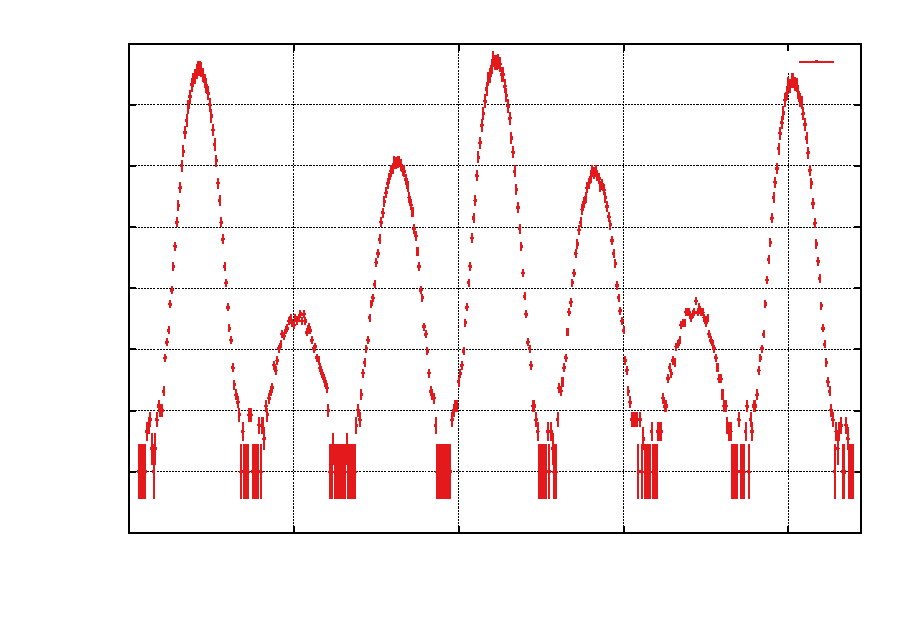
\includegraphics{./plots/HOM/702MHz}}%
    \gplfronttext
  \end{picture}%
\endgroup

  \caption[Feldverteilung der $\mathrm{TE}_{111}$-Mode \mbox{$\nu_0 = \SI{702.70}{MHz}$}]{Verteilung des transversalen elektrischen Feldes der $\mathrm{TE}_{111}$-Mode bei einer Resonanzfrequenz von \mbox{$\nu_0 = \SI{702.70}{MHz}$} im Vakuum.}
\end{figure}

\begin{figure}[p]
	\centering
	
	% GNUPLOT: LaTeX picture with Postscript
\begingroup
  \makeatletter
  \providecommand\color[2][]{%
    \GenericError{(gnuplot) \space\space\space\@spaces}{%
      Package color not loaded in conjunction with
      terminal option `colourtext'%
    }{See the gnuplot documentation for explanation.%
    }{Either use 'blacktext' in gnuplot or load the package
      color.sty in LaTeX.}%
    \renewcommand\color[2][]{}%
  }%
  \providecommand\includegraphics[2][]{%
    \GenericError{(gnuplot) \space\space\space\@spaces}{%
      Package graphicx or graphics not loaded%
    }{See the gnuplot documentation for explanation.%
    }{The gnuplot epslatex terminal needs graphicx.sty or graphics.sty.}%
    \renewcommand\includegraphics[2][]{}%
  }%
  \providecommand\rotatebox[2]{#2}%
  \@ifundefined{ifGPcolor}{%
    \newif\ifGPcolor
    \GPcolortrue
  }{}%
  \@ifundefined{ifGPblacktext}{%
    \newif\ifGPblacktext
    \GPblacktexttrue
  }{}%
  % define a \g@addto@macro without @ in the name:
  \let\gplgaddtomacro\g@addto@macro
  % define empty templates for all commands taking text:
  \gdef\gplbacktext{}%
  \gdef\gplfronttext{}%
  \makeatother
  \ifGPblacktext
    % no textcolor at all
    \def\colorrgb#1{}%
    \def\colorgray#1{}%
  \else
    % gray or color?
    \ifGPcolor
      \def\colorrgb#1{\color[rgb]{#1}}%
      \def\colorgray#1{\color[gray]{#1}}%
      \expandafter\def\csname LTw\endcsname{\color{white}}%
      \expandafter\def\csname LTb\endcsname{\color{black}}%
      \expandafter\def\csname LTa\endcsname{\color{black}}%
      \expandafter\def\csname LT0\endcsname{\color[rgb]{1,0,0}}%
      \expandafter\def\csname LT1\endcsname{\color[rgb]{0,1,0}}%
      \expandafter\def\csname LT2\endcsname{\color[rgb]{0,0,1}}%
      \expandafter\def\csname LT3\endcsname{\color[rgb]{1,0,1}}%
      \expandafter\def\csname LT4\endcsname{\color[rgb]{0,1,1}}%
      \expandafter\def\csname LT5\endcsname{\color[rgb]{1,1,0}}%
      \expandafter\def\csname LT6\endcsname{\color[rgb]{0,0,0}}%
      \expandafter\def\csname LT7\endcsname{\color[rgb]{1,0.3,0}}%
      \expandafter\def\csname LT8\endcsname{\color[rgb]{0.5,0.5,0.5}}%
    \else
      % gray
      \def\colorrgb#1{\color{black}}%
      \def\colorgray#1{\color[gray]{#1}}%
      \expandafter\def\csname LTw\endcsname{\color{white}}%
      \expandafter\def\csname LTb\endcsname{\color{black}}%
      \expandafter\def\csname LTa\endcsname{\color{black}}%
      \expandafter\def\csname LT0\endcsname{\color{black}}%
      \expandafter\def\csname LT1\endcsname{\color{black}}%
      \expandafter\def\csname LT2\endcsname{\color{black}}%
      \expandafter\def\csname LT3\endcsname{\color{black}}%
      \expandafter\def\csname LT4\endcsname{\color{black}}%
      \expandafter\def\csname LT5\endcsname{\color{black}}%
      \expandafter\def\csname LT6\endcsname{\color{black}}%
      \expandafter\def\csname LT7\endcsname{\color{black}}%
      \expandafter\def\csname LT8\endcsname{\color{black}}%
    \fi
  \fi
    \setlength{\unitlength}{0.0500bp}%
    \ifx\gptboxheight\undefined%
      \newlength{\gptboxheight}%
      \newlength{\gptboxwidth}%
      \newsavebox{\gptboxtext}%
    \fi%
    \setlength{\fboxrule}{0.5pt}%
    \setlength{\fboxsep}{1pt}%
\begin{picture}(8502.00,5668.00)%
    \gplgaddtomacro\gplbacktext{%
      \csname LTb\endcsname%
      \put(946,704){\makebox(0,0)[r]{\strut{}-500}}%
      \csname LTb\endcsname%
      \put(946,1226){\makebox(0,0)[r]{\strut{}0}}%
      \csname LTb\endcsname%
      \put(946,1748){\makebox(0,0)[r]{\strut{}500}}%
      \csname LTb\endcsname%
      \put(946,2270){\makebox(0,0)[r]{\strut{}1000}}%
      \csname LTb\endcsname%
      \put(946,2792){\makebox(0,0)[r]{\strut{}1500}}%
      \csname LTb\endcsname%
      \put(946,3315){\makebox(0,0)[r]{\strut{}2000}}%
      \csname LTb\endcsname%
      \put(946,3837){\makebox(0,0)[r]{\strut{}2500}}%
      \csname LTb\endcsname%
      \put(946,4359){\makebox(0,0)[r]{\strut{}3000}}%
      \csname LTb\endcsname%
      \put(946,4881){\makebox(0,0)[r]{\strut{}3500}}%
      \csname LTb\endcsname%
      \put(946,5403){\makebox(0,0)[r]{\strut{}4000}}%
      \csname LTb\endcsname%
      \put(1078,484){\makebox(0,0){\strut{}0}}%
      \csname LTb\endcsname%
      \put(2661,484){\makebox(0,0){\strut{}500}}%
      \csname LTb\endcsname%
      \put(4243,484){\makebox(0,0){\strut{}1000}}%
      \csname LTb\endcsname%
      \put(5826,484){\makebox(0,0){\strut{}1500}}%
      \csname LTb\endcsname%
      \put(7409,484){\makebox(0,0){\strut{}2000}}%
    }%
    \gplgaddtomacro\gplfronttext{%
      \csname LTb\endcsname%
      \put(176,3053){\rotatebox{-270}{\makebox(0,0){\strut{}$\frac{E_0(z)}{\sqrt{P_\mathrm{V}}}$ / \si{\volt\per\metre\per\watt\tothe{0.5}}}}}%
      \put(4591,154){\makebox(0,0){\strut{}$z$ / \si{mm}}}%
      \csname LTb\endcsname%
      \put(7382,5230){\makebox(0,0)[r]{\strut{}Amplitude}}%
    }%
    \gplbacktext
    \put(0,0){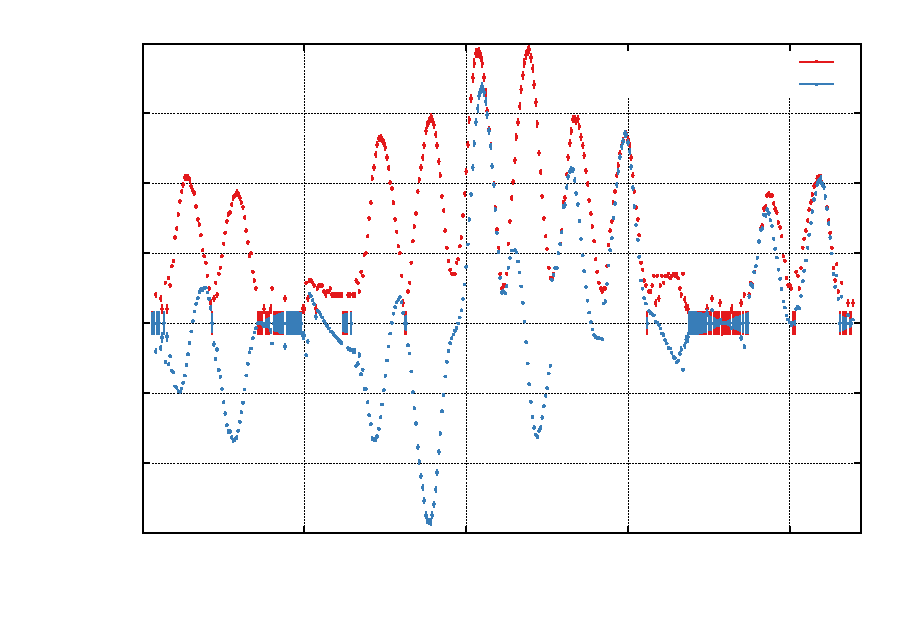
\includegraphics{./plots/HOM/730MHz}}%
    \gplfronttext
  \end{picture}%
\endgroup

	\caption[Feldverteilung der $\mathrm{TM}_{011}$-Mode \mbox{$\nu_0 = \SI{730.45}{MHz}$}]{Verteilung des longitudinalen elektrischen Feldes der $\mathrm{TM}_{011}$-Mode bei einer Resonanzfrequenz von \mbox{$\nu_0 = \SI{730.45}{MHz}$} im Vakuum.}
	
	% GNUPLOT: LaTeX picture with Postscript
\begingroup
  \makeatletter
  \providecommand\color[2][]{%
    \GenericError{(gnuplot) \space\space\space\@spaces}{%
      Package color not loaded in conjunction with
      terminal option `colourtext'%
    }{See the gnuplot documentation for explanation.%
    }{Either use 'blacktext' in gnuplot or load the package
      color.sty in LaTeX.}%
    \renewcommand\color[2][]{}%
  }%
  \providecommand\includegraphics[2][]{%
    \GenericError{(gnuplot) \space\space\space\@spaces}{%
      Package graphicx or graphics not loaded%
    }{See the gnuplot documentation for explanation.%
    }{The gnuplot epslatex terminal needs graphicx.sty or graphics.sty.}%
    \renewcommand\includegraphics[2][]{}%
  }%
  \providecommand\rotatebox[2]{#2}%
  \@ifundefined{ifGPcolor}{%
    \newif\ifGPcolor
    \GPcolortrue
  }{}%
  \@ifundefined{ifGPblacktext}{%
    \newif\ifGPblacktext
    \GPblacktexttrue
  }{}%
  % define a \g@addto@macro without @ in the name:
  \let\gplgaddtomacro\g@addto@macro
  % define empty templates for all commands taking text:
  \gdef\gplbacktext{}%
  \gdef\gplfronttext{}%
  \makeatother
  \ifGPblacktext
    % no textcolor at all
    \def\colorrgb#1{}%
    \def\colorgray#1{}%
  \else
    % gray or color?
    \ifGPcolor
      \def\colorrgb#1{\color[rgb]{#1}}%
      \def\colorgray#1{\color[gray]{#1}}%
      \expandafter\def\csname LTw\endcsname{\color{white}}%
      \expandafter\def\csname LTb\endcsname{\color{black}}%
      \expandafter\def\csname LTa\endcsname{\color{black}}%
      \expandafter\def\csname LT0\endcsname{\color[rgb]{1,0,0}}%
      \expandafter\def\csname LT1\endcsname{\color[rgb]{0,1,0}}%
      \expandafter\def\csname LT2\endcsname{\color[rgb]{0,0,1}}%
      \expandafter\def\csname LT3\endcsname{\color[rgb]{1,0,1}}%
      \expandafter\def\csname LT4\endcsname{\color[rgb]{0,1,1}}%
      \expandafter\def\csname LT5\endcsname{\color[rgb]{1,1,0}}%
      \expandafter\def\csname LT6\endcsname{\color[rgb]{0,0,0}}%
      \expandafter\def\csname LT7\endcsname{\color[rgb]{1,0.3,0}}%
      \expandafter\def\csname LT8\endcsname{\color[rgb]{0.5,0.5,0.5}}%
    \else
      % gray
      \def\colorrgb#1{\color{black}}%
      \def\colorgray#1{\color[gray]{#1}}%
      \expandafter\def\csname LTw\endcsname{\color{white}}%
      \expandafter\def\csname LTb\endcsname{\color{black}}%
      \expandafter\def\csname LTa\endcsname{\color{black}}%
      \expandafter\def\csname LT0\endcsname{\color{black}}%
      \expandafter\def\csname LT1\endcsname{\color{black}}%
      \expandafter\def\csname LT2\endcsname{\color{black}}%
      \expandafter\def\csname LT3\endcsname{\color{black}}%
      \expandafter\def\csname LT4\endcsname{\color{black}}%
      \expandafter\def\csname LT5\endcsname{\color{black}}%
      \expandafter\def\csname LT6\endcsname{\color{black}}%
      \expandafter\def\csname LT7\endcsname{\color{black}}%
      \expandafter\def\csname LT8\endcsname{\color{black}}%
    \fi
  \fi
    \setlength{\unitlength}{0.0500bp}%
    \ifx\gptboxheight\undefined%
      \newlength{\gptboxheight}%
      \newlength{\gptboxwidth}%
      \newsavebox{\gptboxtext}%
    \fi%
    \setlength{\fboxrule}{0.5pt}%
    \setlength{\fboxsep}{1pt}%
\begin{picture}(8502.00,5668.00)%
    \gplgaddtomacro\gplbacktext{%
      \csname LTb\endcsname%
      \put(1078,704){\makebox(0,0)[r]{\strut{}-5000}}%
      \csname LTb\endcsname%
      \put(1078,1174){\makebox(0,0)[r]{\strut{}-4000}}%
      \csname LTb\endcsname%
      \put(1078,1644){\makebox(0,0)[r]{\strut{}-3000}}%
      \csname LTb\endcsname%
      \put(1078,2114){\makebox(0,0)[r]{\strut{}-2000}}%
      \csname LTb\endcsname%
      \put(1078,2584){\makebox(0,0)[r]{\strut{}-1000}}%
      \csname LTb\endcsname%
      \put(1078,3054){\makebox(0,0)[r]{\strut{}0}}%
      \csname LTb\endcsname%
      \put(1078,3523){\makebox(0,0)[r]{\strut{}1000}}%
      \csname LTb\endcsname%
      \put(1078,3993){\makebox(0,0)[r]{\strut{}2000}}%
      \csname LTb\endcsname%
      \put(1078,4463){\makebox(0,0)[r]{\strut{}3000}}%
      \csname LTb\endcsname%
      \put(1078,4933){\makebox(0,0)[r]{\strut{}4000}}%
      \csname LTb\endcsname%
      \put(1078,5403){\makebox(0,0)[r]{\strut{}5000}}%
      \csname LTb\endcsname%
      \put(1210,484){\makebox(0,0){\strut{}0}}%
      \csname LTb\endcsname%
      \put(2763,484){\makebox(0,0){\strut{}500}}%
      \csname LTb\endcsname%
      \put(4316,484){\makebox(0,0){\strut{}1000}}%
      \csname LTb\endcsname%
      \put(5869,484){\makebox(0,0){\strut{}1500}}%
      \csname LTb\endcsname%
      \put(7422,484){\makebox(0,0){\strut{}2000}}%
    }%
    \gplgaddtomacro\gplfronttext{%
      \csname LTb\endcsname%
      \put(176,3053){\rotatebox{-270}{\makebox(0,0){\strut{}$\frac{E_0(z)}{\sqrt{P_\mathrm{V}}}$ / \si{\volt\per\metre\per\watt\tothe{0{,}5}}}}}%
      \put(4657,154){\makebox(0,0){\strut{}$z$ / \si{mm}}}%
      \csname LTb\endcsname%
      \put(7382,5230){\makebox(0,0)[r]{\strut{}Amplitude}}%
      \csname LTb\endcsname%
      \put(7382,5010){\makebox(0,0)[r]{\strut{}effektives Feld}}%
    }%
    \gplbacktext
    \put(0,0){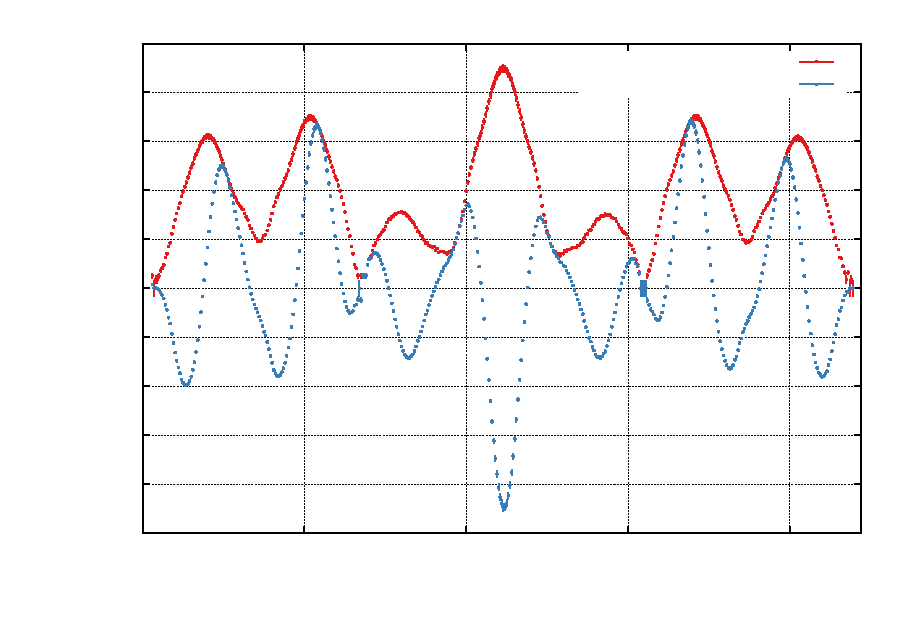
\includegraphics{./plots/HOM/1047MHz}}%
    \gplfronttext
  \end{picture}%
\endgroup

	\caption[Feldverteilung der $\mathrm{TM}_{111}$-Mode \mbox{$\nu_0 = \SI{1047.23}{MHz}$}]{Verteilung des transversalen elektrischen Feldes der $\mathrm{TM}_{111}$-Mode bei einer Resonanzfrequenz von \mbox{$\nu_0 = \SI{1047.23}{MHz}$} im Vakuum.}
\end{figure}

\begin{figure}[p]
	\centering
	
	% GNUPLOT: LaTeX picture with Postscript
\begingroup
  \makeatletter
  \providecommand\color[2][]{%
    \GenericError{(gnuplot) \space\space\space\@spaces}{%
      Package color not loaded in conjunction with
      terminal option `colourtext'%
    }{See the gnuplot documentation for explanation.%
    }{Either use 'blacktext' in gnuplot or load the package
      color.sty in LaTeX.}%
    \renewcommand\color[2][]{}%
  }%
  \providecommand\includegraphics[2][]{%
    \GenericError{(gnuplot) \space\space\space\@spaces}{%
      Package graphicx or graphics not loaded%
    }{See the gnuplot documentation for explanation.%
    }{The gnuplot epslatex terminal needs graphicx.sty or graphics.sty.}%
    \renewcommand\includegraphics[2][]{}%
  }%
  \providecommand\rotatebox[2]{#2}%
  \@ifundefined{ifGPcolor}{%
    \newif\ifGPcolor
    \GPcolortrue
  }{}%
  \@ifundefined{ifGPblacktext}{%
    \newif\ifGPblacktext
    \GPblacktexttrue
  }{}%
  % define a \g@addto@macro without @ in the name:
  \let\gplgaddtomacro\g@addto@macro
  % define empty templates for all commands taking text:
  \gdef\gplbacktext{}%
  \gdef\gplfronttext{}%
  \makeatother
  \ifGPblacktext
    % no textcolor at all
    \def\colorrgb#1{}%
    \def\colorgray#1{}%
  \else
    % gray or color?
    \ifGPcolor
      \def\colorrgb#1{\color[rgb]{#1}}%
      \def\colorgray#1{\color[gray]{#1}}%
      \expandafter\def\csname LTw\endcsname{\color{white}}%
      \expandafter\def\csname LTb\endcsname{\color{black}}%
      \expandafter\def\csname LTa\endcsname{\color{black}}%
      \expandafter\def\csname LT0\endcsname{\color[rgb]{1,0,0}}%
      \expandafter\def\csname LT1\endcsname{\color[rgb]{0,1,0}}%
      \expandafter\def\csname LT2\endcsname{\color[rgb]{0,0,1}}%
      \expandafter\def\csname LT3\endcsname{\color[rgb]{1,0,1}}%
      \expandafter\def\csname LT4\endcsname{\color[rgb]{0,1,1}}%
      \expandafter\def\csname LT5\endcsname{\color[rgb]{1,1,0}}%
      \expandafter\def\csname LT6\endcsname{\color[rgb]{0,0,0}}%
      \expandafter\def\csname LT7\endcsname{\color[rgb]{1,0.3,0}}%
      \expandafter\def\csname LT8\endcsname{\color[rgb]{0.5,0.5,0.5}}%
    \else
      % gray
      \def\colorrgb#1{\color{black}}%
      \def\colorgray#1{\color[gray]{#1}}%
      \expandafter\def\csname LTw\endcsname{\color{white}}%
      \expandafter\def\csname LTb\endcsname{\color{black}}%
      \expandafter\def\csname LTa\endcsname{\color{black}}%
      \expandafter\def\csname LT0\endcsname{\color{black}}%
      \expandafter\def\csname LT1\endcsname{\color{black}}%
      \expandafter\def\csname LT2\endcsname{\color{black}}%
      \expandafter\def\csname LT3\endcsname{\color{black}}%
      \expandafter\def\csname LT4\endcsname{\color{black}}%
      \expandafter\def\csname LT5\endcsname{\color{black}}%
      \expandafter\def\csname LT6\endcsname{\color{black}}%
      \expandafter\def\csname LT7\endcsname{\color{black}}%
      \expandafter\def\csname LT8\endcsname{\color{black}}%
    \fi
  \fi
    \setlength{\unitlength}{0.0500bp}%
    \ifx\gptboxheight\undefined%
      \newlength{\gptboxheight}%
      \newlength{\gptboxwidth}%
      \newsavebox{\gptboxtext}%
    \fi%
    \setlength{\fboxrule}{0.5pt}%
    \setlength{\fboxsep}{1pt}%
\begin{picture}(8502.00,5668.00)%
    \gplgaddtomacro\gplbacktext{%
      \csname LTb\endcsname%
      \put(1078,704){\makebox(0,0)[r]{\strut{}-1000}}%
      \csname LTb\endcsname%
      \put(1078,1487){\makebox(0,0)[r]{\strut{}0}}%
      \csname LTb\endcsname%
      \put(1078,2270){\makebox(0,0)[r]{\strut{}1000}}%
      \csname LTb\endcsname%
      \put(1078,3054){\makebox(0,0)[r]{\strut{}2000}}%
      \csname LTb\endcsname%
      \put(1078,3837){\makebox(0,0)[r]{\strut{}3000}}%
      \csname LTb\endcsname%
      \put(1078,4620){\makebox(0,0)[r]{\strut{}4000}}%
      \csname LTb\endcsname%
      \put(1078,5403){\makebox(0,0)[r]{\strut{}5000}}%
      \csname LTb\endcsname%
      \put(1210,484){\makebox(0,0){\strut{}0}}%
      \csname LTb\endcsname%
      \put(2763,484){\makebox(0,0){\strut{}500}}%
      \csname LTb\endcsname%
      \put(4316,484){\makebox(0,0){\strut{}1000}}%
      \csname LTb\endcsname%
      \put(5869,484){\makebox(0,0){\strut{}1500}}%
      \csname LTb\endcsname%
      \put(7422,484){\makebox(0,0){\strut{}2000}}%
    }%
    \gplgaddtomacro\gplfronttext{%
      \csname LTb\endcsname%
      \put(176,3053){\rotatebox{-270}{\makebox(0,0){\strut{}$\frac{E_0(z)}{\sqrt{P_\mathrm{V}}}$ / \si{\volt\per\metre\per\watt\tothe{0.5}}}}}%
      \put(4657,154){\makebox(0,0){\strut{}$z$ / \si{mm}}}%
      \csname LTb\endcsname%
      \put(7382,5230){\makebox(0,0)[r]{\strut{}Amplitude}}%
    }%
    \gplbacktext
    \put(0,0){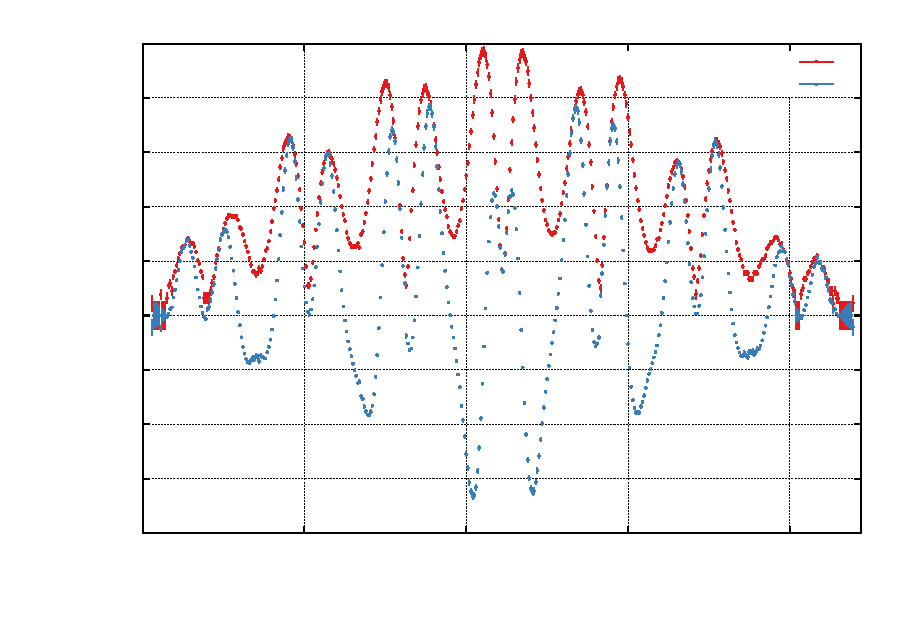
\includegraphics{./plots/HOM/1375MHz}}%
    \gplfronttext
  \end{picture}%
\endgroup

	\caption[Feldverteilung der $\mathrm{TM}$-Mode \mbox{$\nu_0 = \SI{1375.79}{MHz}$}]{Verteilung des longitudinalen elektrischen Feldes der $\mathrm{TM}$-Mode bei einer Resonanzfrequenz von \mbox{$\nu_0 = \SI{1375.79}{MHz}$} im Vakuum.}
	
    % GNUPLOT: LaTeX picture with Postscript
\begingroup
  \makeatletter
  \providecommand\color[2][]{%
    \GenericError{(gnuplot) \space\space\space\@spaces}{%
      Package color not loaded in conjunction with
      terminal option `colourtext'%
    }{See the gnuplot documentation for explanation.%
    }{Either use 'blacktext' in gnuplot or load the package
      color.sty in LaTeX.}%
    \renewcommand\color[2][]{}%
  }%
  \providecommand\includegraphics[2][]{%
    \GenericError{(gnuplot) \space\space\space\@spaces}{%
      Package graphicx or graphics not loaded%
    }{See the gnuplot documentation for explanation.%
    }{The gnuplot epslatex terminal needs graphicx.sty or graphics.sty.}%
    \renewcommand\includegraphics[2][]{}%
  }%
  \providecommand\rotatebox[2]{#2}%
  \@ifundefined{ifGPcolor}{%
    \newif\ifGPcolor
    \GPcolortrue
  }{}%
  \@ifundefined{ifGPblacktext}{%
    \newif\ifGPblacktext
    \GPblacktexttrue
  }{}%
  % define a \g@addto@macro without @ in the name:
  \let\gplgaddtomacro\g@addto@macro
  % define empty templates for all commands taking text:
  \gdef\gplbacktext{}%
  \gdef\gplfronttext{}%
  \makeatother
  \ifGPblacktext
    % no textcolor at all
    \def\colorrgb#1{}%
    \def\colorgray#1{}%
  \else
    % gray or color?
    \ifGPcolor
      \def\colorrgb#1{\color[rgb]{#1}}%
      \def\colorgray#1{\color[gray]{#1}}%
      \expandafter\def\csname LTw\endcsname{\color{white}}%
      \expandafter\def\csname LTb\endcsname{\color{black}}%
      \expandafter\def\csname LTa\endcsname{\color{black}}%
      \expandafter\def\csname LT0\endcsname{\color[rgb]{1,0,0}}%
      \expandafter\def\csname LT1\endcsname{\color[rgb]{0,1,0}}%
      \expandafter\def\csname LT2\endcsname{\color[rgb]{0,0,1}}%
      \expandafter\def\csname LT3\endcsname{\color[rgb]{1,0,1}}%
      \expandafter\def\csname LT4\endcsname{\color[rgb]{0,1,1}}%
      \expandafter\def\csname LT5\endcsname{\color[rgb]{1,1,0}}%
      \expandafter\def\csname LT6\endcsname{\color[rgb]{0,0,0}}%
      \expandafter\def\csname LT7\endcsname{\color[rgb]{1,0.3,0}}%
      \expandafter\def\csname LT8\endcsname{\color[rgb]{0.5,0.5,0.5}}%
    \else
      % gray
      \def\colorrgb#1{\color{black}}%
      \def\colorgray#1{\color[gray]{#1}}%
      \expandafter\def\csname LTw\endcsname{\color{white}}%
      \expandafter\def\csname LTb\endcsname{\color{black}}%
      \expandafter\def\csname LTa\endcsname{\color{black}}%
      \expandafter\def\csname LT0\endcsname{\color{black}}%
      \expandafter\def\csname LT1\endcsname{\color{black}}%
      \expandafter\def\csname LT2\endcsname{\color{black}}%
      \expandafter\def\csname LT3\endcsname{\color{black}}%
      \expandafter\def\csname LT4\endcsname{\color{black}}%
      \expandafter\def\csname LT5\endcsname{\color{black}}%
      \expandafter\def\csname LT6\endcsname{\color{black}}%
      \expandafter\def\csname LT7\endcsname{\color{black}}%
      \expandafter\def\csname LT8\endcsname{\color{black}}%
    \fi
  \fi
    \setlength{\unitlength}{0.0500bp}%
    \ifx\gptboxheight\undefined%
      \newlength{\gptboxheight}%
      \newlength{\gptboxwidth}%
      \newsavebox{\gptboxtext}%
    \fi%
    \setlength{\fboxrule}{0.5pt}%
    \setlength{\fboxsep}{1pt}%
\begin{picture}(8502.00,5668.00)%
    \gplgaddtomacro\gplbacktext{%
      \csname LTb\endcsname%
      \put(1078,704){\makebox(0,0)[r]{\strut{}-2000}}%
      \csname LTb\endcsname%
      \put(1078,1226){\makebox(0,0)[r]{\strut{}-1500}}%
      \csname LTb\endcsname%
      \put(1078,1748){\makebox(0,0)[r]{\strut{}-1000}}%
      \csname LTb\endcsname%
      \put(1078,2270){\makebox(0,0)[r]{\strut{}-500}}%
      \csname LTb\endcsname%
      \put(1078,2792){\makebox(0,0)[r]{\strut{}0}}%
      \csname LTb\endcsname%
      \put(1078,3315){\makebox(0,0)[r]{\strut{}500}}%
      \csname LTb\endcsname%
      \put(1078,3837){\makebox(0,0)[r]{\strut{}1000}}%
      \csname LTb\endcsname%
      \put(1078,4359){\makebox(0,0)[r]{\strut{}1500}}%
      \csname LTb\endcsname%
      \put(1078,4881){\makebox(0,0)[r]{\strut{}2000}}%
      \csname LTb\endcsname%
      \put(1078,5403){\makebox(0,0)[r]{\strut{}2500}}%
      \csname LTb\endcsname%
      \put(1210,484){\makebox(0,0){\strut{}0}}%
      \csname LTb\endcsname%
      \put(2763,484){\makebox(0,0){\strut{}500}}%
      \csname LTb\endcsname%
      \put(4316,484){\makebox(0,0){\strut{}1000}}%
      \csname LTb\endcsname%
      \put(5869,484){\makebox(0,0){\strut{}1500}}%
      \csname LTb\endcsname%
      \put(7422,484){\makebox(0,0){\strut{}2000}}%
    }%
    \gplgaddtomacro\gplfronttext{%
      \csname LTb\endcsname%
      \put(176,3053){\rotatebox{-270}{\makebox(0,0){\strut{}$\frac{E_0(z)}{\sqrt{P_\mathrm{V}}}$ / \si{\volt\per\metre\per\watt\tothe{0.5}}}}}%
      \put(4657,154){\makebox(0,0){\strut{}$z$ / \si{mm}}}%
      \csname LTb\endcsname%
      \put(7382,5230){\makebox(0,0)[r]{\strut{}Amplitude}}%
      \csname LTb\endcsname%
      \put(7382,5010){\makebox(0,0)[r]{\strut{}effektives Feld}}%
    }%
    \gplbacktext
    \put(0,0){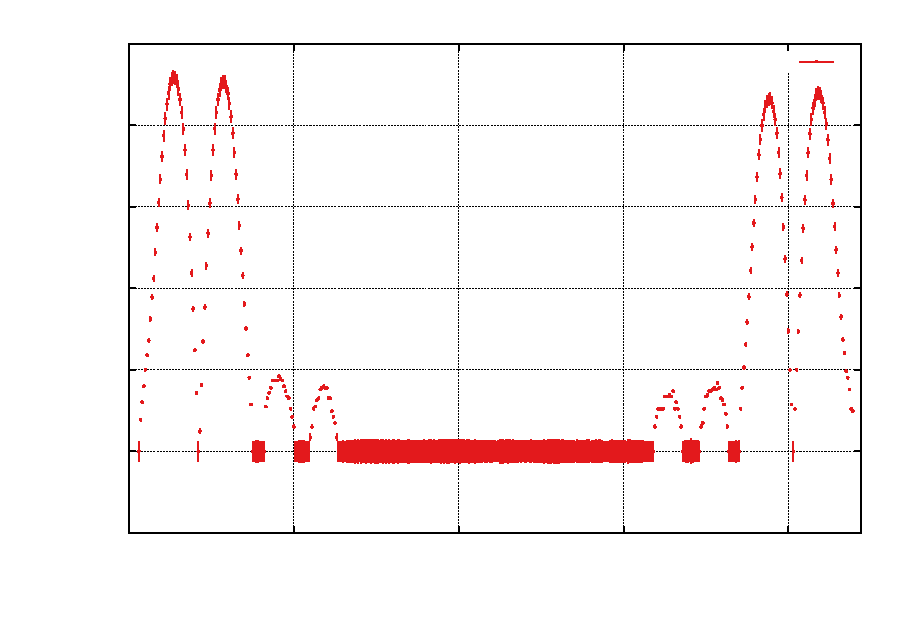
\includegraphics{./plots/HOM/1458MHz}}%
    \gplfronttext
  \end{picture}%
\endgroup

    \caption[Feldverteilung der $\mathrm{TM}_{021}$-Mode \mbox{$\nu_0 = \SI{1458.30}{MHz}$}]{Verteilung des longitudinalen elektrischen Feldes der $\mathrm{TM}_{021}$-Mode bei einer Resonanzfrequenz von \mbox{$\nu_0 = \SI{1458.30}{MHz}$} im Vakuum.}
    \label{fig:tm021_1458}
\end{figure}

\begin{figure}[p]
	\centering
	% GNUPLOT: LaTeX picture with Postscript
\begingroup
  \makeatletter
  \providecommand\color[2][]{%
    \GenericError{(gnuplot) \space\space\space\@spaces}{%
      Package color not loaded in conjunction with
      terminal option `colourtext'%
    }{See the gnuplot documentation for explanation.%
    }{Either use 'blacktext' in gnuplot or load the package
      color.sty in LaTeX.}%
    \renewcommand\color[2][]{}%
  }%
  \providecommand\includegraphics[2][]{%
    \GenericError{(gnuplot) \space\space\space\@spaces}{%
      Package graphicx or graphics not loaded%
    }{See the gnuplot documentation for explanation.%
    }{The gnuplot epslatex terminal needs graphicx.sty or graphics.sty.}%
    \renewcommand\includegraphics[2][]{}%
  }%
  \providecommand\rotatebox[2]{#2}%
  \@ifundefined{ifGPcolor}{%
    \newif\ifGPcolor
    \GPcolortrue
  }{}%
  \@ifundefined{ifGPblacktext}{%
    \newif\ifGPblacktext
    \GPblacktexttrue
  }{}%
  % define a \g@addto@macro without @ in the name:
  \let\gplgaddtomacro\g@addto@macro
  % define empty templates for all commands taking text:
  \gdef\gplbacktext{}%
  \gdef\gplfronttext{}%
  \makeatother
  \ifGPblacktext
    % no textcolor at all
    \def\colorrgb#1{}%
    \def\colorgray#1{}%
  \else
    % gray or color?
    \ifGPcolor
      \def\colorrgb#1{\color[rgb]{#1}}%
      \def\colorgray#1{\color[gray]{#1}}%
      \expandafter\def\csname LTw\endcsname{\color{white}}%
      \expandafter\def\csname LTb\endcsname{\color{black}}%
      \expandafter\def\csname LTa\endcsname{\color{black}}%
      \expandafter\def\csname LT0\endcsname{\color[rgb]{1,0,0}}%
      \expandafter\def\csname LT1\endcsname{\color[rgb]{0,1,0}}%
      \expandafter\def\csname LT2\endcsname{\color[rgb]{0,0,1}}%
      \expandafter\def\csname LT3\endcsname{\color[rgb]{1,0,1}}%
      \expandafter\def\csname LT4\endcsname{\color[rgb]{0,1,1}}%
      \expandafter\def\csname LT5\endcsname{\color[rgb]{1,1,0}}%
      \expandafter\def\csname LT6\endcsname{\color[rgb]{0,0,0}}%
      \expandafter\def\csname LT7\endcsname{\color[rgb]{1,0.3,0}}%
      \expandafter\def\csname LT8\endcsname{\color[rgb]{0.5,0.5,0.5}}%
    \else
      % gray
      \def\colorrgb#1{\color{black}}%
      \def\colorgray#1{\color[gray]{#1}}%
      \expandafter\def\csname LTw\endcsname{\color{white}}%
      \expandafter\def\csname LTb\endcsname{\color{black}}%
      \expandafter\def\csname LTa\endcsname{\color{black}}%
      \expandafter\def\csname LT0\endcsname{\color{black}}%
      \expandafter\def\csname LT1\endcsname{\color{black}}%
      \expandafter\def\csname LT2\endcsname{\color{black}}%
      \expandafter\def\csname LT3\endcsname{\color{black}}%
      \expandafter\def\csname LT4\endcsname{\color{black}}%
      \expandafter\def\csname LT5\endcsname{\color{black}}%
      \expandafter\def\csname LT6\endcsname{\color{black}}%
      \expandafter\def\csname LT7\endcsname{\color{black}}%
      \expandafter\def\csname LT8\endcsname{\color{black}}%
    \fi
  \fi
    \setlength{\unitlength}{0.0500bp}%
    \ifx\gptboxheight\undefined%
      \newlength{\gptboxheight}%
      \newlength{\gptboxwidth}%
      \newsavebox{\gptboxtext}%
    \fi%
    \setlength{\fboxrule}{0.5pt}%
    \setlength{\fboxsep}{1pt}%
\begin{picture}(8502.00,5668.00)%
    \gplgaddtomacro\gplbacktext{%
      \csname LTb\endcsname%
      \put(946,704){\makebox(0,0)[r]{\strut{}-500}}%
      \csname LTb\endcsname%
      \put(946,1487){\makebox(0,0)[r]{\strut{}0}}%
      \csname LTb\endcsname%
      \put(946,2270){\makebox(0,0)[r]{\strut{}500}}%
      \csname LTb\endcsname%
      \put(946,3054){\makebox(0,0)[r]{\strut{}1000}}%
      \csname LTb\endcsname%
      \put(946,3837){\makebox(0,0)[r]{\strut{}1500}}%
      \csname LTb\endcsname%
      \put(946,4620){\makebox(0,0)[r]{\strut{}2000}}%
      \csname LTb\endcsname%
      \put(946,5403){\makebox(0,0)[r]{\strut{}2500}}%
      \csname LTb\endcsname%
      \put(1078,484){\makebox(0,0){\strut{}0}}%
      \csname LTb\endcsname%
      \put(2661,484){\makebox(0,0){\strut{}500}}%
      \csname LTb\endcsname%
      \put(4243,484){\makebox(0,0){\strut{}1000}}%
      \csname LTb\endcsname%
      \put(5826,484){\makebox(0,0){\strut{}1500}}%
      \csname LTb\endcsname%
      \put(7409,484){\makebox(0,0){\strut{}2000}}%
    }%
    \gplgaddtomacro\gplfronttext{%
      \csname LTb\endcsname%
      \put(176,3053){\rotatebox{-270}{\makebox(0,0){\strut{}$\frac{E_0(z)}{\sqrt{P_\mathrm{V}}}$ / \si{\volt\per\metre\per\watt\tothe{0.5}}}}}%
      \put(4591,154){\makebox(0,0){\strut{}$z$ / \si{mm}}}%
      \csname LTb\endcsname%
      \put(7382,5230){\makebox(0,0)[r]{\strut{}Amplitude}}%
    }%
    \gplbacktext
    \put(0,0){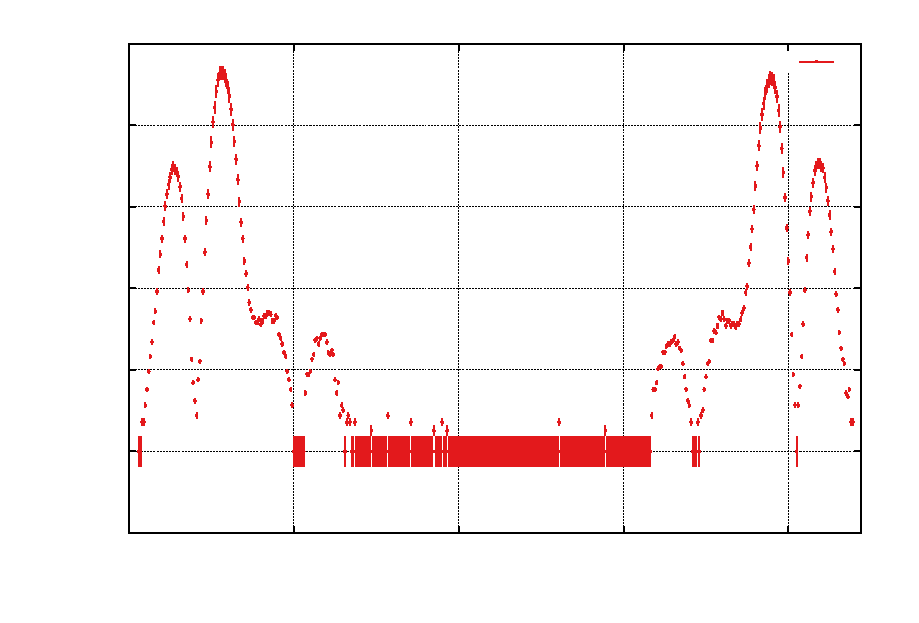
\includegraphics{./plots/HOM/1460MHz}}%
    \gplfronttext
  \end{picture}%
\endgroup

	\caption[Feldverteilung der $\mathrm{TM}_{021}$-Mode \mbox{$\nu_0 = \SI{1460.34}{MHz}$}]{Verteilung des longitudinalen elektrischen Feldes der $\mathrm{TM}_{021}$-Mode bei einer Resonanzfrequenz von \mbox{$\nu_0 = \SI{1460.34}{MHz}$} im Vakuum.}
	\label{fig:tm021_1460}
    
    % GNUPLOT: LaTeX picture with Postscript
\begingroup
  \makeatletter
  \providecommand\color[2][]{%
    \GenericError{(gnuplot) \space\space\space\@spaces}{%
      Package color not loaded in conjunction with
      terminal option `colourtext'%
    }{See the gnuplot documentation for explanation.%
    }{Either use 'blacktext' in gnuplot or load the package
      color.sty in LaTeX.}%
    \renewcommand\color[2][]{}%
  }%
  \providecommand\includegraphics[2][]{%
    \GenericError{(gnuplot) \space\space\space\@spaces}{%
      Package graphicx or graphics not loaded%
    }{See the gnuplot documentation for explanation.%
    }{The gnuplot epslatex terminal needs graphicx.sty or graphics.sty.}%
    \renewcommand\includegraphics[2][]{}%
  }%
  \providecommand\rotatebox[2]{#2}%
  \@ifundefined{ifGPcolor}{%
    \newif\ifGPcolor
    \GPcolortrue
  }{}%
  \@ifundefined{ifGPblacktext}{%
    \newif\ifGPblacktext
    \GPblacktexttrue
  }{}%
  % define a \g@addto@macro without @ in the name:
  \let\gplgaddtomacro\g@addto@macro
  % define empty templates for all commands taking text:
  \gdef\gplbacktext{}%
  \gdef\gplfronttext{}%
  \makeatother
  \ifGPblacktext
    % no textcolor at all
    \def\colorrgb#1{}%
    \def\colorgray#1{}%
  \else
    % gray or color?
    \ifGPcolor
      \def\colorrgb#1{\color[rgb]{#1}}%
      \def\colorgray#1{\color[gray]{#1}}%
      \expandafter\def\csname LTw\endcsname{\color{white}}%
      \expandafter\def\csname LTb\endcsname{\color{black}}%
      \expandafter\def\csname LTa\endcsname{\color{black}}%
      \expandafter\def\csname LT0\endcsname{\color[rgb]{1,0,0}}%
      \expandafter\def\csname LT1\endcsname{\color[rgb]{0,1,0}}%
      \expandafter\def\csname LT2\endcsname{\color[rgb]{0,0,1}}%
      \expandafter\def\csname LT3\endcsname{\color[rgb]{1,0,1}}%
      \expandafter\def\csname LT4\endcsname{\color[rgb]{0,1,1}}%
      \expandafter\def\csname LT5\endcsname{\color[rgb]{1,1,0}}%
      \expandafter\def\csname LT6\endcsname{\color[rgb]{0,0,0}}%
      \expandafter\def\csname LT7\endcsname{\color[rgb]{1,0.3,0}}%
      \expandafter\def\csname LT8\endcsname{\color[rgb]{0.5,0.5,0.5}}%
    \else
      % gray
      \def\colorrgb#1{\color{black}}%
      \def\colorgray#1{\color[gray]{#1}}%
      \expandafter\def\csname LTw\endcsname{\color{white}}%
      \expandafter\def\csname LTb\endcsname{\color{black}}%
      \expandafter\def\csname LTa\endcsname{\color{black}}%
      \expandafter\def\csname LT0\endcsname{\color{black}}%
      \expandafter\def\csname LT1\endcsname{\color{black}}%
      \expandafter\def\csname LT2\endcsname{\color{black}}%
      \expandafter\def\csname LT3\endcsname{\color{black}}%
      \expandafter\def\csname LT4\endcsname{\color{black}}%
      \expandafter\def\csname LT5\endcsname{\color{black}}%
      \expandafter\def\csname LT6\endcsname{\color{black}}%
      \expandafter\def\csname LT7\endcsname{\color{black}}%
      \expandafter\def\csname LT8\endcsname{\color{black}}%
    \fi
  \fi
    \setlength{\unitlength}{0.0500bp}%
    \ifx\gptboxheight\undefined%
      \newlength{\gptboxheight}%
      \newlength{\gptboxwidth}%
      \newsavebox{\gptboxtext}%
    \fi%
    \setlength{\fboxrule}{0.5pt}%
    \setlength{\fboxsep}{1pt}%
\begin{picture}(8502.00,5668.00)%
    \gplgaddtomacro\gplbacktext{%
      \csname LTb\endcsname%
      \put(1078,704){\makebox(0,0)[r]{\strut{}-2500}}%
      \csname LTb\endcsname%
      \put(1078,1174){\makebox(0,0)[r]{\strut{}-2000}}%
      \csname LTb\endcsname%
      \put(1078,1644){\makebox(0,0)[r]{\strut{}-1500}}%
      \csname LTb\endcsname%
      \put(1078,2114){\makebox(0,0)[r]{\strut{}-1000}}%
      \csname LTb\endcsname%
      \put(1078,2584){\makebox(0,0)[r]{\strut{}-500}}%
      \csname LTb\endcsname%
      \put(1078,3054){\makebox(0,0)[r]{\strut{}0}}%
      \csname LTb\endcsname%
      \put(1078,3523){\makebox(0,0)[r]{\strut{}500}}%
      \csname LTb\endcsname%
      \put(1078,3993){\makebox(0,0)[r]{\strut{}1000}}%
      \csname LTb\endcsname%
      \put(1078,4463){\makebox(0,0)[r]{\strut{}1500}}%
      \csname LTb\endcsname%
      \put(1078,4933){\makebox(0,0)[r]{\strut{}2000}}%
      \csname LTb\endcsname%
      \put(1078,5403){\makebox(0,0)[r]{\strut{}2500}}%
      \csname LTb\endcsname%
      \put(1210,484){\makebox(0,0){\strut{}0}}%
      \csname LTb\endcsname%
      \put(2763,484){\makebox(0,0){\strut{}500}}%
      \csname LTb\endcsname%
      \put(4316,484){\makebox(0,0){\strut{}1000}}%
      \csname LTb\endcsname%
      \put(5869,484){\makebox(0,0){\strut{}1500}}%
      \csname LTb\endcsname%
      \put(7422,484){\makebox(0,0){\strut{}2000}}%
    }%
    \gplgaddtomacro\gplfronttext{%
      \csname LTb\endcsname%
      \put(176,3053){\rotatebox{-270}{\makebox(0,0){\strut{}$\frac{E_0(z)}{\sqrt{P_\mathrm{V}}}$ / \si{\volt\per\metre\per\watt\tothe{0.5}}}}}%
      \put(4657,154){\makebox(0,0){\strut{}$z$ / \si{mm}}}%
      \csname LTb\endcsname%
      \put(7382,5230){\makebox(0,0)[r]{\strut{}Amplitude}}%
      \csname LTb\endcsname%
      \put(7382,5010){\makebox(0,0)[r]{\strut{}effektives Feld}}%
    }%
    \gplbacktext
    \put(0,0){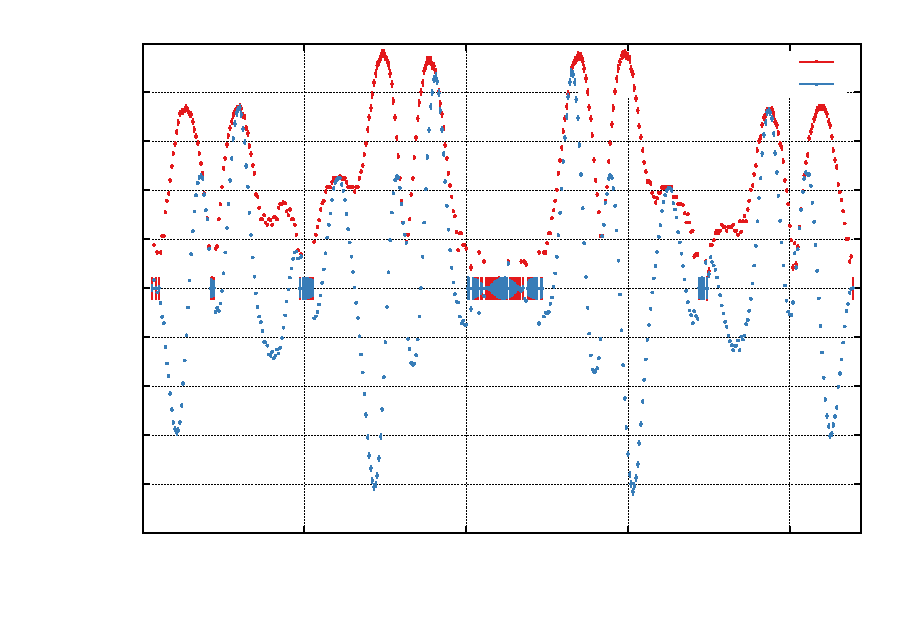
\includegraphics{./plots/HOM/1465_L_MHz}}%
    \gplfronttext
  \end{picture}%
\endgroup

    \caption[Feldverteilung der $\mathrm{TM}_{021}$-Mode \mbox{$\nu_0 = \SI{1464.96}{MHz}$}]{Verteilung des longitudinalen elektrischen Feldes der $\mathrm{TM}_{021}$-Mode bei einer Resonanzfrequenz von \mbox{$\nu_0 = \SI{1464.96}{MHz}$} im Vakuum.}
\end{figure}


\begin{figure}[p]
  \centering
  % GNUPLOT: LaTeX picture with Postscript
\begingroup
  \makeatletter
  \providecommand\color[2][]{%
    \GenericError{(gnuplot) \space\space\space\@spaces}{%
      Package color not loaded in conjunction with
      terminal option `colourtext'%
    }{See the gnuplot documentation for explanation.%
    }{Either use 'blacktext' in gnuplot or load the package
      color.sty in LaTeX.}%
    \renewcommand\color[2][]{}%
  }%
  \providecommand\includegraphics[2][]{%
    \GenericError{(gnuplot) \space\space\space\@spaces}{%
      Package graphicx or graphics not loaded%
    }{See the gnuplot documentation for explanation.%
    }{The gnuplot epslatex terminal needs graphicx.sty or graphics.sty.}%
    \renewcommand\includegraphics[2][]{}%
  }%
  \providecommand\rotatebox[2]{#2}%
  \@ifundefined{ifGPcolor}{%
    \newif\ifGPcolor
    \GPcolortrue
  }{}%
  \@ifundefined{ifGPblacktext}{%
    \newif\ifGPblacktext
    \GPblacktexttrue
  }{}%
  % define a \g@addto@macro without @ in the name:
  \let\gplgaddtomacro\g@addto@macro
  % define empty templates for all commands taking text:
  \gdef\gplbacktext{}%
  \gdef\gplfronttext{}%
  \makeatother
  \ifGPblacktext
    % no textcolor at all
    \def\colorrgb#1{}%
    \def\colorgray#1{}%
  \else
    % gray or color?
    \ifGPcolor
      \def\colorrgb#1{\color[rgb]{#1}}%
      \def\colorgray#1{\color[gray]{#1}}%
      \expandafter\def\csname LTw\endcsname{\color{white}}%
      \expandafter\def\csname LTb\endcsname{\color{black}}%
      \expandafter\def\csname LTa\endcsname{\color{black}}%
      \expandafter\def\csname LT0\endcsname{\color[rgb]{1,0,0}}%
      \expandafter\def\csname LT1\endcsname{\color[rgb]{0,1,0}}%
      \expandafter\def\csname LT2\endcsname{\color[rgb]{0,0,1}}%
      \expandafter\def\csname LT3\endcsname{\color[rgb]{1,0,1}}%
      \expandafter\def\csname LT4\endcsname{\color[rgb]{0,1,1}}%
      \expandafter\def\csname LT5\endcsname{\color[rgb]{1,1,0}}%
      \expandafter\def\csname LT6\endcsname{\color[rgb]{0,0,0}}%
      \expandafter\def\csname LT7\endcsname{\color[rgb]{1,0.3,0}}%
      \expandafter\def\csname LT8\endcsname{\color[rgb]{0.5,0.5,0.5}}%
    \else
      % gray
      \def\colorrgb#1{\color{black}}%
      \def\colorgray#1{\color[gray]{#1}}%
      \expandafter\def\csname LTw\endcsname{\color{white}}%
      \expandafter\def\csname LTb\endcsname{\color{black}}%
      \expandafter\def\csname LTa\endcsname{\color{black}}%
      \expandafter\def\csname LT0\endcsname{\color{black}}%
      \expandafter\def\csname LT1\endcsname{\color{black}}%
      \expandafter\def\csname LT2\endcsname{\color{black}}%
      \expandafter\def\csname LT3\endcsname{\color{black}}%
      \expandafter\def\csname LT4\endcsname{\color{black}}%
      \expandafter\def\csname LT5\endcsname{\color{black}}%
      \expandafter\def\csname LT6\endcsname{\color{black}}%
      \expandafter\def\csname LT7\endcsname{\color{black}}%
      \expandafter\def\csname LT8\endcsname{\color{black}}%
    \fi
  \fi
    \setlength{\unitlength}{0.0500bp}%
    \ifx\gptboxheight\undefined%
      \newlength{\gptboxheight}%
      \newlength{\gptboxwidth}%
      \newsavebox{\gptboxtext}%
    \fi%
    \setlength{\fboxrule}{0.5pt}%
    \setlength{\fboxsep}{1pt}%
\begin{picture}(8502.00,5668.00)%
    \gplgaddtomacro\gplbacktext{%
      \csname LTb\endcsname%
      \put(1078,704){\makebox(0,0)[r]{\strut{}-1500}}%
      \csname LTb\endcsname%
      \put(1078,1291){\makebox(0,0)[r]{\strut{}-1000}}%
      \csname LTb\endcsname%
      \put(1078,1879){\makebox(0,0)[r]{\strut{}-500}}%
      \csname LTb\endcsname%
      \put(1078,2466){\makebox(0,0)[r]{\strut{}0}}%
      \csname LTb\endcsname%
      \put(1078,3054){\makebox(0,0)[r]{\strut{}500}}%
      \csname LTb\endcsname%
      \put(1078,3641){\makebox(0,0)[r]{\strut{}1000}}%
      \csname LTb\endcsname%
      \put(1078,4228){\makebox(0,0)[r]{\strut{}1500}}%
      \csname LTb\endcsname%
      \put(1078,4816){\makebox(0,0)[r]{\strut{}2000}}%
      \csname LTb\endcsname%
      \put(1078,5403){\makebox(0,0)[r]{\strut{}2500}}%
      \csname LTb\endcsname%
      \put(1210,484){\makebox(0,0){\strut{}0}}%
      \csname LTb\endcsname%
      \put(2763,484){\makebox(0,0){\strut{}500}}%
      \csname LTb\endcsname%
      \put(4316,484){\makebox(0,0){\strut{}1000}}%
      \csname LTb\endcsname%
      \put(5869,484){\makebox(0,0){\strut{}1500}}%
      \csname LTb\endcsname%
      \put(7422,484){\makebox(0,0){\strut{}2000}}%
    }%
    \gplgaddtomacro\gplfronttext{%
      \csname LTb\endcsname%
      \put(176,3053){\rotatebox{-270}{\makebox(0,0){\strut{}$\frac{E_0(z)}{\sqrt{P_\mathrm{V}}}$ / \si{\volt\per\metre\per\watt\tothe{0.5}}}}}%
      \put(4657,154){\makebox(0,0){\strut{}$z$ / \si{mm}}}%
      \csname LTb\endcsname%
      \put(7382,5230){\makebox(0,0)[r]{\strut{}Amplitude}}%
      \csname LTb\endcsname%
      \put(7382,5010){\makebox(0,0)[r]{\strut{}effektives Feld}}%
    }%
    \gplbacktext
    \put(0,0){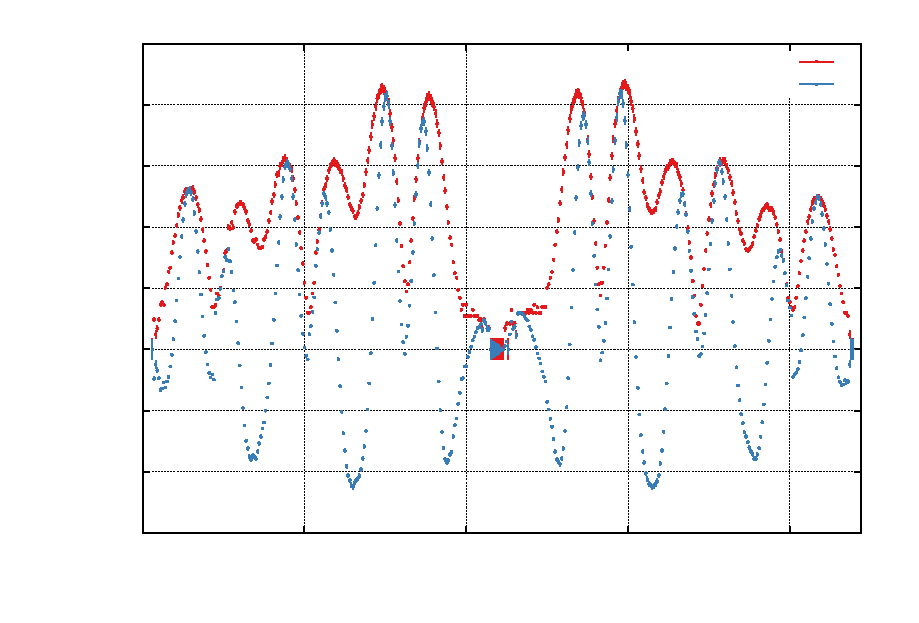
\includegraphics{./plots/HOM/1465_R_MHz}}%
    \gplfronttext
  \end{picture}%
\endgroup

  \caption[Feldverteilung der $\mathrm{TM}_{021}$-Mode \mbox{$\nu_0 = \SI{1465.83}{MHz}$}]{Verteilung des longitudinalen elektrischen Feldes der $\mathrm{TM}_{021}$-Mode bei einer Resonanzfrequenz von \mbox{$\nu_0 = \SI{1465.83}{MHz}$} im Vakuum.}
\end{figure}


\FloatBarrier
% \printbibliography[heading=subbibliography]

\backmatter
%------------------------------------------------------------------------------
% Declare bibliography, lists of figures and tables and
% acknowledgements as backmatter
% Chapter/section numbers are turned off

%------------------------------------------------------------------------------
% Include the following lines and comment out \printbibliography if
% you use BiBTeX for the bibliography.
% If you use biblatex package the files should be specified in the preamble.
%
% {\raggedright
%   \bibliographystyle{unsrt}
%   \bibliography{./thesis_refs,../refs/standard_refs-bibtex}
% }

%------------------------------------------------------------------------------
% Use biblatex for the bibliography
% Add bibliography to Table of Contents
% Comment out this command if your references are printed for each chapter.
\printbibliography[heading=bibintoc]

\listoffigures
%\listoftables

%------------------------------------------------------------------------------
% Print the glossary and list of acronyms
% \printglossaries

%------------------------------------------------------------------------------
% You could instead add your acknowledgements here - don't forget to
% also add them to \includeonly above
%------------------------------------------------------------------------------
\chapter*{Danksagung}
\label{sec:danksagung}
%------------------------------------------------------------------------------
Diese Arbeit wurde erst durch die tatkräftige Unterstützung vieler Personen möglich.
Daher richtet sich mein Dank an:
\begin{itemize}
	\item Herrn Priv.-Doz.\ Dr.\ Wolfgang Hillert für das Überlassen dieses interessanten Arbeitsthemas und der Möglichkeit des selbstständigen Arbeitens.
	
	\item Herrn Prof.\ Dr.\ Klaus Desch für die bereitwillige Übernahme des Koreferats.
	
	\item Jens Derksen für seine guten Ideen und eine angenehme Büroatmosphäre.
	
	\item Dennis Sauerland und Manuel Schedler für die tatkräftige Unterstützung und Betreuung dieser Arbeit.
	
	\item Herrn Philipp Hänisch und Herrn Michael Brock, die trotz zahlreicher Verpflichtungen stets Zeit gefunden haben, um mir bei technischen Problemen zu helfen.
	
	\item Nikolas Heurich und Dennis Proft für das Korrekturlesen dieser Arbeit.
	
	\item Die restliche Arbeitsgruppe von ELSA für das angenehme Arbeitsklima und ständige Hilfsbereitschaft bei allen aufgekommenen Fragen.
	
	\item Meiner Familie und allen, die mich auf meinem Weg unterstützt haben.
\end{itemize}
Abschließend richtet sich mein herzlicher Dank auch an alle Personen, die nicht erwähnt wurden.

\end{document}
